\documentclass[12pt,a4paper]{article}

\usepackage[margin=2.5cm]{geometry}
\usepackage{cite}
\usepackage{algorithmic}
\usepackage{graphicx}
\usepackage{textcomp}
\usepackage{xcolor}
\usepackage{url}
\usepackage{amsmath,amsxtra,amssymb,amsthm,latexsym,amscd,amsfonts}
\usepackage[utf8]{vietnam}
\usepackage[english]{babel}
\usepackage{fancyhdr}
\usepackage{multirow}
\usepackage{booktabs}
\usepackage{tabularx}
\usepackage{longtable}
\usepackage{float}
\pagestyle{fancy}

\fancyhf{}
\fancyfoot[C]{\thepage}
\renewcommand{\headrulewidth}{0pt}
\renewcommand{\footrulewidth}{0pt}

\def\BibTeX{{\rm B\kern-.05em{\sc i\kern-.025em b}\kern-.08em
    T\kern-.1667em\lower.7ex\hbox{E}\kern-.125emX}}

\begin{document}

\title{SCA-MobileNet: Kiến trúc học sâu cho xác thực tĩnh mạch lòng bàn tay không tiếp xúc với khối SCIB}

\author{Nguyễn Quốc Vương, Huỳnh Minh Quân, Bùi Danh Hường, và Hoàng Văn Quý%
\thanks{Nguyễn Quốc Vương và Huỳnh Minh Quân là sinh viên Khoa Công nghệ Thông tin, Trường Đại học Công nghệ TP.HCM (HUTECH), TP.HCM, Việt Nam (e-mail: vug10032004@gmail.com; hquan8696@gmail.com).}%
\thanks{Bùi Danh Hường công tác tại Trường Đại học Công nghệ TP.HCM (HUTECH), TP.HCM, Việt Nam (e-mail: bd.huong@hutech.edu.vn).}%
\thanks{Hoàng Văn Quý công tác tại Trường Đại học Thủy lợi (Thuyloi University), TP.HCM, Việt Nam (e-mail: hoangvanquy@tlu.edu.vn).}%
}

\maketitle


\begin{abstract}
Nghiên cứu này đề xuất SCA-MobileNet, một kiến trúc xác thực tĩnh mạch lòng bàn tay không tiếp xúc theo giao thức tập mở (open-set), giải quyết vấn đề biến thiên tỷ lệ hình học do khoảng cách thu nhận thay đổi. Hệ thống bao gồm: (i) quy trình tiền xử lý ba giai đoạn --- phân đoạn tự động, chuẩn hóa tỷ lệ dựa trên phép biến đổi khoảng cách, và tăng cường CLAHE; và (ii) kiến trúc mạng SCA-MobileNet. Kiến trúc tích hợp khối SCIB (Scale-Coordinate Invariant Block) gồm Coordinate Attention (CA) và Spatial Pyramid Pooling (SPP) trên nền MobileNetV3-Small rút gọn, kết hợp Spatial Transformer Network (STN) tại đầu vào và hàm mất mát AdaCos. Đánh giá trên bốn bộ dữ liệu với 11 kiến trúc baseline cho kết quả: EER 0,89\% trên bộ nội bộ (1.549 ID), 0,06\% trên TONGJI, 1,48\% trên SCUT, 2,76\% trên VERA --- xếp hạng \#1 trên tất cả 7 kịch bản (4 in-domain + 3 cross-domain) với 3,19M tham số và 0,13G FLOPs.
\end{abstract}

\medskip
\noindent\textbf{Từ khóa:} palm vein authentication, SCA-MobileNet, MobileNetV3, Spatial Transformer Network, Coordinate Attention, Spatial Pyramid Pooling, open-set verification.

%% ====== SECTION I ======
\section{Giới thiệu}

Trong bối cảnh chuyển đổi số và yêu cầu giảm thiểu tiếp xúc vật lý sau đại dịch COVID-19, sinh trắc học không tiếp xúc (\textit{contactless biometrics}) ngày càng được quan tâm \cite{b_covid1}. Xác thực tĩnh mạch lòng bàn tay (\textit{palm vein biometrics}) là một trong những phương thức có tính bảo mật cao nhờ mẫu mạch máu phân bố hoàn toàn bên dưới bề mặt da \cite{b_covid2}. Khác với các đặc trưng bề mặt như khuôn mặt, mống mắt hay vân tay \cite{b18}, \cite{b19}, cấu trúc tĩnh mạch chỉ có thể thu nhận qua ánh sáng hồng ngoại gần (NIR, dải $760\text{--}850\text{nm}$), nơi hemoglobin khử oxy hấp thụ mạnh bức xạ. Đặc điểm này khiến việc giả mạo mẫu trở nên khó khăn hơn đáng kể so với các phương thức sinh trắc bề mặt \cite{b5}. Ngoài ra, tĩnh mạch ít bị ảnh hưởng bởi các khiếm khuyết da (sẹo, mồ hôi, mài mòn), đảm bảo tính bền vững lâu dài.

Tuy nhiên, việc chuyển từ hệ thống quét tiếp xúc (\textit{contact-based sensors}) sang thu nhận không tiếp xúc đặt ra nhiều thách thức về thị giác máy tính \cite{b1}. Khi không có chốt vật lý dẫn hướng, hệ thống phải xử lý các biến thiên về tư thế bàn tay, cường độ chiếu sáng, và đặc biệt là biến thiên tỷ lệ hình học (\textit{scale variation}) do khoảng cách thu nhận không cố định. Sự thay đổi khoảng cách này làm biến đổi kích thước biểu kiến của lòng bàn tay trên ảnh, ảnh hưởng trực tiếp đến tính nhất quán của đặc trưng tĩnh mạch.

Vấn đề này trở nên nghiêm trọng hơn trong giao thức đánh giá tập mở (\textit{open-set recognition}) \cite{b12}, \cite{b13}. Khác với bài toán phân loại tập đóng, hệ thống open-set phải xử lý các danh tính chưa từng xuất hiện trong quá trình huấn luyện. Mô hình không đóng vai trò bộ phân loại mà phải trích xuất vector embedding sao cho các mẫu cùng danh tính gần nhau trong không gian metric. Nếu tính nhất quán tỷ lệ bị phá vỡ, embedding của cùng một bàn tay ở các khoảng cách khác nhau sẽ phân kỳ, làm tăng tỷ lệ từ chối sai (FRR).

Phần lớn các nghiên cứu hiện tại xử lý biến thiên tỷ lệ bằng cách resize vùng ROI về kích thước cố định trước khi đưa vào mạng \cite{b1}, \cite{b4}. Cách tiếp cận này giả định CNN sẽ tự học bù đắp biến dạng hình học, nhưng thực tế CNN thiếu cơ chế nội tại để thiết lập tính bất biến tỷ lệ tường minh.

Để giải quyết vấn đề này, nghiên cứu đề xuất SCA-MobileNet với hai thành phần chính:

Thứ nhất, quy trình tiền xử lý sử dụng phép biến đổi khoảng cách (\textit{Distance Transform}) để xác định tâm lòng bàn tay và trích xuất ROI với tỷ lệ thích ứng ($k \cdot L$), bảo toàn tỷ lệ pixel nội tại của cấu trúc tĩnh mạch. Bước tăng cường CLAHE được áp dụng tiếp theo để cải thiện tương phản cục bộ.

Thứ hai, kiến trúc mạng SCA-MobileNet xây dựng trên nền MobileNetV3-Small \cite{b10} với khối SCIB (Scale-Coordinate Invariant Block). SCIB tích hợp tuần tự: (i) mạng chuyển đổi không gian STN \cite{b9} để chuẩn hóa hình học đầu vào, (ii) cơ chế Chú ý Tọa độ (CA) \cite{b7} để định vị chính xác các nhánh tĩnh mạch theo trục không gian, và (iii) Phân tích kim tự tháp không gian (SPP) \cite{b8} để tạo biểu diễn đa thang đo. Hàm mất mát AdaCos \cite{b11} với tham số tỷ lệ tự động được sử dụng để tối ưu không gian embedding.

Các đóng góp chính của công trình:
\begin{enumerate}
    \item Đề xuất quy trình chuẩn hóa tỷ lệ dựa trên phép biến đổi khoảng cách, cho phép trích xuất ROI thích ứng mà không làm biến dạng cấu trúc tĩnh mạch.
    \item Thiết kế khối SCIB tích hợp STN, CA và SPP trên nền MobileNetV3-Small, đạt hiệu năng cao với chỉ 3,19M tham số.
    \item Đánh giá toàn diện trên bốn bộ dữ liệu theo giao thức open-set identity-disjoint: EER 0,89\% trên bộ nội bộ (1.549 ID), 0,06\% trên TONGJI, 1,48\% trên SCUT, và 2,76\% trên VERA --- xếp hạng nhất trên tất cả 7 kịch bản bao gồm đánh giá cross-domain.
    \item Công bố toàn bộ mã nguồn và cấu hình huấn luyện để đảm bảo tính tái lập.
\end{enumerate}

%% ====== SECTION II ======
\section{Tổng quan Nghiên cứu và Cơ sở Lý thuyết}

\subsection{Bài toán Xác thực Tập mở (Open-Set Verification)}
Trong sinh trắc học ứng dụng, giao thức đánh giá tập mở (\textit{open-set}) yêu cầu hệ thống xử lý các danh tính chưa xuất hiện trong quá trình huấn luyện. Scheirer và cộng sự \cite{b12} định nghĩa hệ thống open-set phải có khả năng từ chối ngoại lai (\textit{rejection of unknowns}), nghĩa là mô hình cần tạo ra biểu diễn embedding có biên phân tách rõ ràng cho cả các lớp chưa quan sát.

Trong giao thức này, hệ thống tính toán khoảng cách (cosine hoặc L2) giữa embedding của ảnh đầu vào và template tham chiếu. Nếu khoảng cách nhỏ hơn ngưỡng quy định (ví dụ tại FAR = 0,01\%), cá nhân được xác thực. Điều này đòi hỏi mô hình phải học biểu diễn tổng quát thay vì chỉ phân loại các lớp đã biết. Giao thức \textit{Identity-Disjoint Split} \cite{b13} --- trong đó tập huấn luyện và kiểm thử không chia sẻ bất kỳ danh tính nào --- được sử dụng trong nghiên cứu này để đảm bảo đánh giá phản ánh đúng điều kiện thực tế.

\subsection{Hàm mất mát Angular Margin và AdaCos}
Các nghiên cứu ban đầu về nhận dạng tĩnh mạch sử dụng hàm Softmax Cross-Entropy \cite{b1}, \cite{b_closedset}. Softmax tối ưu ranh giới phân tách giữa các lớp đã biết nhưng không trực tiếp thúc đẩy tính gom tụ nội lớp (\textit{intra-class compactness}), dẫn đến hiệu năng kém trong điều kiện open-set khi các cụm đặc trưng có thể chồng lấn.

Các hàm mất mát dựa trên lề lượng giác (\textit{angular margin losses}) như ArcFace \cite{b14}, CosFace \cite{b15} và SphereFace \cite{b16} giải quyết vấn đề này bằng cách ánh xạ embedding lên mặt siêu cầu và thêm biên phạt góc. Kuzu và cộng sự \cite{b2} đã áp dụng thành công ArcFace cho tĩnh mạch. Tuy nhiên, các hàm này phụ thuộc vào siêu tham số $scale~s$ và $margin~m$, đòi hỏi điều chỉnh cẩn thận theo từng bộ dữ liệu.

SCA-MobileNet sử dụng biến thể của \textbf{AdaCos} \cite{b11}, trong đó tham số tỷ lệ $s$ được tính tự động: $s = \sqrt{2} \cdot \log(C - 1)$, với $C$ là số lớp. Khác với AdaCos gốc (không sử dụng biên cố định), nghiên cứu bổ sung biên góc cộng $m = 0{,}35$ (tương tự ArcFace \cite{b14}) nhằm tăng cường tính gom tụ nội lớp. Kết hợp với optimizer AdamW, cấu hình này loại bỏ nhu cầu điều chỉnh thủ công $s$ và cho phép huấn luyện ổn định trên các bộ dữ liệu có quy mô khác nhau.

\subsection{Học Đặc trưng Đa thang đo và các Công trình Liên quan}
Trong lĩnh vực nhận dạng tĩnh mạch, nhiều kiến trúc đã được đề xuất để xử lý biến dạng cục bộ. RSNet \cite{b4} sử dụng kiến trúc Siamese hai nhánh (global + local patches), đạt EER thấp nhưng có chi phí tính toán cao, hạn chế khả năng triển khai trên thiết bị biên. GSCL \cite{b3} áp dụng học tự giám sát (\textit{self-supervised learning}) với dữ liệu tổng hợp, đạt kết quả tốt trên PolyU nhưng đòi hỏi quy trình huấn luyện phức tạp. FGFNet \cite{b5} tích hợp FFT vào lớp chập để xử lý nhiễu tần số. Cần lưu ý rằng FGFNet ban đầu được thiết kế cho bài toán phát hiện tấn công giả mạo (\textit{presentation attack detection} --- PAD); trong nghiên cứu này, backbone MobileViT kết hợp FFC của FGFNet được thích ứng (\textit{adapt}) sang trích xuất đặc trưng cho bài toán xác thực sinh trắc.

SCA-MobileNet tiếp cận khác biệt bằng cách tích hợp tính bất biến tỷ lệ trực tiếp vào kiến trúc thông qua khối SCIB. SPP \cite{b8} tạo biểu diễn đa thang đo $(1\times 1, 2\times 2, 4\times 4)$ mà không cần nhân bản backbone, trong khi CA \cite{b7} định vị đặc trưng theo trục không gian. Sự kết hợp này cho phép backbone nhẹ MobileNetV3-Small (3,19M tham số) đạt hiệu năng cạnh tranh với các kiến trúc lớn hơn đáng kể.

\subsection{Chuẩn hóa Tỷ lệ tại Tiền xử lý}
Hầu hết các hệ thống tĩnh mạch không tiếp xúc trích xuất ROI dựa trên tọa độ cố định (ví dụ vị trí khe ngón tay) \cite{b1}. Phương pháp này nhạy cảm với biến thiên khoảng cách thu nhận: chỉ cần thay đổi 1cm chiều sâu có thể làm thay đổi đáng kể kích thước biểu kiến của mạng tĩnh mạch. Việc resize về kích thước cố định sau đó sẽ làm biến dạng tỷ lệ giữa các mạch máu.

Nghiên cứu này sử dụng phép biến đổi khoảng cách (\textit{Distance Transform}) để xác định tâm lòng bàn tay và độ dài tham chiếu nội tại $L$. ROI được trích xuất với kích thước $k \cdot L$, duy trì tỷ lệ hình học nhất quán bất kể khoảng cách thu nhận. Kết hợp với tăng cường CLAHE và augmentation dữ liệu, quy trình này cung cấp đầu vào chuẩn hóa cho mạng STN ở giai đoạn tiếp theo.

%% ====== SECTION III ======
\section{Cơ sở dữ liệu đánh giá}

Để đánh giá toàn diện khả năng tổng quát hóa của hệ thống trên nhiều phương thức thu nhận, vùng giải phẫu, và quy mô dữ liệu, chúng tôi tiến hành thực nghiệm trên \textbf{bốn bộ dữ liệu}: (1) bộ dữ liệu tĩnh mạch lòng bàn tay NIR tự thu thập quy mô lớn (1.549 định danh); (2) bộ dữ liệu vân lòng bàn tay TONGJI công khai (1.200 định danh, ánh sáng khả kiến); (3) bộ dữ liệu vân lòng bàn tay SCUT FVP công khai (1.100 định danh, ánh sáng khả kiến); và (4) bộ dữ liệu tĩnh mạch lòng bàn tay VERA công khai (220 định danh, NIR). Việc đưa bộ dữ liệu vân lòng bàn tay (palmprint) vào đánh giá nhằm kiểm chứng tính tổng quát hóa của kiến trúc đề xuất trên nhiều dạng kết cấu sinh trắc (\textit{biometric texture}): cả tĩnh mạch (vein) và vân da (palmprint) đều mang cấu trúc đường nét hình học đặc trưng cho từng cá nhân, chỉ khác nhau về phương thức thu nhận (NIR vs.\ ánh sáng khả kiến). Ba bộ dữ liệu công khai (TONGJI, SCUT, VERA) \textbf{đã cung cấp sẵn vùng ROI cắt trích}, do đó chỉ cần áp dụng bước tăng cường CLAHE và chuẩn hóa Z-score trước khi đưa vào mô hình. Riêng bộ dữ liệu nội bộ yêu cầu pipeline tiền xử lý đầy đủ ba giai đoạn (phân đoạn GrabCut $\rightarrow$ trích xuất ROI + chuẩn hóa Distance Transform $\rightarrow$ CLAHE).

\subsection{Bộ dữ liệu Tự thu thập}

\begin{figure}[H]
\centerline{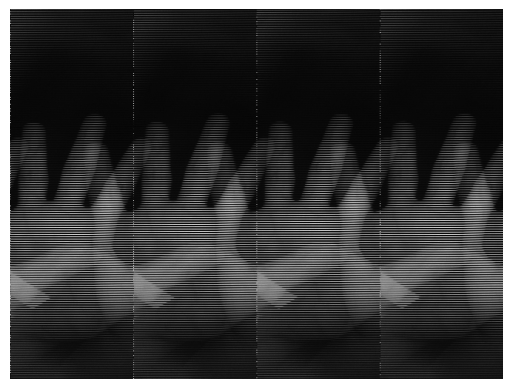
\includegraphics[width=\columnwidth]{fig_pose_variation.png}}
\caption{Minh họa sự biến thiên về tư thế và khoảng cách của lòng bàn tay trong quá trình thu nhận không tiếp xúc (bộ dữ liệu tự thu thập).}
\label{fig:pose_variation}
\end{figure}

Cơ sở dữ liệu tĩnh mạch lòng bàn tay nội bộ được thu thập từ 1.549 người tình nguyện thông qua cảm biến hồng ngoại gần (NIR, bước sóng 850nm) theo phương thức không tiếp xúc. Hemoglobin khử oxy trong máu tĩnh mạch hấp thụ mạnh ánh sáng ở bước sóng này, tạo ra ảnh có độ tương phản cao của mạng mạch máu dưới da. Dữ liệu từ tay trái và tay phải được xử lý như các định danh độc lập, mỗi bàn tay cung cấp 10 mẫu ảnh, tổng cộng 15.490 ảnh ở định dạng nhị phân 640×480 pixel. Tập dữ liệu được chia thành 1.084 định danh huấn luyện và 465 định danh kiểm thử theo giao thức identity-disjoint.

\subsection{Bộ dữ liệu TONGJI Contactless Palmprint}

Để đánh giá khả năng tổng quát hóa trên các phương thức thu nhận khác nhau, chúng tôi sử dụng bộ dữ liệu TONGJI Contactless Palmprint \cite{b21}. Mặc dù TONGJI chứa ảnh vân lòng bàn tay dưới ánh sáng khả kiến thay vì tĩnh mạch NIR, cả hai đặc trưng đều dựa trên cấu trúc đường nét hình học. TONGJI gồm 12.000 ảnh ROI ($128 \times 128$ pixel) từ 600 cá nhân (1.200 định danh), thu thập qua hai phiên cách nhau trung bình 2 tháng. Kịch bản open-set: 840 định danh huấn luyện và 360 định danh kiểm thử.

\subsection{Bộ dữ liệu SCUT FVP (Contactless Palmprint)}

Bộ dữ liệu SCUT Finger Vein and Palmprint (SCUT FVP) \cite{b_scut} được thu thập bởi Đại học Công nghệ Hoa Nam (South China University of Technology). Bộ dữ liệu bao gồm ảnh vân lòng bàn tay ánh sáng khả kiến (\textit{visible light palmprint}) từ 550 cá nhân, phân tách tay trái/phải thành \textbf{1.100 định danh}. Mỗi định danh cung cấp 10 mẫu ảnh, tổng cộng \textbf{11.000 ảnh} ROI kích thước $128 \times 128$ pixel.

Tương tự TONGJI, ảnh SCUT đã được cắt ROI sẵn, do đó quy trình tiền xử lý chỉ áp dụng CLAHE tăng cường quang học và chuẩn hóa Z-score trước khi đưa vào mô hình. Kịch bản open-set chia tập ở cấp độ danh tính: \textbf{770 định danh huấn luyện} (7.700 ảnh) và \textbf{330 định danh kiểm thử} (3.300 ảnh). Với mỗi định danh 10 mẫu, số cặp genuine: $\binom{10}{2} \times 330 = 14.850$ cặp, impostor được lấy mẫu cân bằng 1:1, tổng cộng \textbf{29.700 phép so khớp}.

SCUT là bộ dữ liệu có quy mô lớn nhất trong các bộ dữ liệu công khai được sử dụng, cho phép đánh giá năng lực phân biệt của các kiến trúc trên không gian định danh rộng.

\subsection{Bộ dữ liệu VERA Palmvein}

Bộ dữ liệu VERA Palmvein \cite{b_vera} được thu thập bởi Idiap Research Institute (Thụy Sĩ) sử dụng cảm biến hồng ngoại gần (NIR) chuyên dụng. Bộ dữ liệu bao gồm ảnh tĩnh mạch lòng bàn tay từ 110 cá nhân, phân tách tay trái/phải thành \textbf{220 định danh}. Mỗi định danh cung cấp 5 mẫu ảnh, tổng cộng \textbf{1.100 ảnh}.

VERA có hai đặc điểm liên quan đến thiết kế thực nghiệm: (1) phương thức NIR trùng với bộ nội bộ nhưng khác TONGJI/SCUT (visible light); và (2) quy mô nhỏ hơn (220 so với 1.100--1.549 định danh), tạo điều kiện đánh giá khả năng học embedding với số lượng lớp hạn chế. Kịch bản open-set: \textbf{154 định danh huấn luyện} (770 ảnh) và \textbf{66 định danh kiểm thử} (330 ảnh). Số cặp genuine: $\binom{5}{2} \times 66 = 660$ cặp, impostor cân bằng 1:1, tổng cộng \textbf{1.320 phép so khớp}.

Do quy mô mẫu kiểm thử nhỏ, các chỉ số TAR@FAR thấp cần được diễn giải thận trọng hơn so với các bộ dữ liệu lớn. Tuy nhiên, VERA đóng vai trò quan trọng trong thí nghiệm cross-domain vì cùng phương thức NIR với tập nội bộ.

\subsection{Tổng hợp Bộ dữ liệu Thực nghiệm}

Bảng~\ref{tab:dataset_summary} tổng hợp các thông số kỹ thuật và giao thức chia tập của bốn bộ dữ liệu được sử dụng trong nghiên cứu.

\begin{table}[H]
\caption{Tổng hợp bốn bộ dữ liệu thực nghiệm và giao thức chia tập open-set.}
\begin{center}
\resizebox{\textwidth}{!}{%
\begin{tabular}{l|c|c|c|c|c|c|c|c}
\hline
\textbf{Bộ dữ liệu} & \textbf{Phương thức} & \textbf{Đặc trưng sinh trắc} & \textbf{Định danh} & \textbf{Mẫu/ID} & \textbf{Tổng ảnh} & \textbf{Train IDs} & \textbf{Test IDs} & \textbf{Cặp so khớp} \\
\hline
Nội bộ (Đề xuất) & NIR 850nm & Tĩnh mạch lòng bàn tay & 1.549 & 10 & 15.490 & 1.084 & 465 & 41.850 \\
TONGJI \cite{b21} & Visible & Vân lòng bàn tay (palmprint) & 1.200 & 10 & 12.000 & 840 & 360 & 32.400 \\
SCUT FVP \cite{b_scut} & Visible & Vân lòng bàn tay (palmprint) & 1.100 & 10 & 11.000 & 770 & 330 & 29.700 \\
VERA \cite{b_vera} & NIR & Tĩnh mạch lòng bàn tay & 220 & 5 & 1.100 & 154 & 66 & 1.320 \\
\hline
\end{tabular}%
}
\label{tab:dataset_summary}
\end{center}
\end{table}

\begin{figure}[H]
\centerline{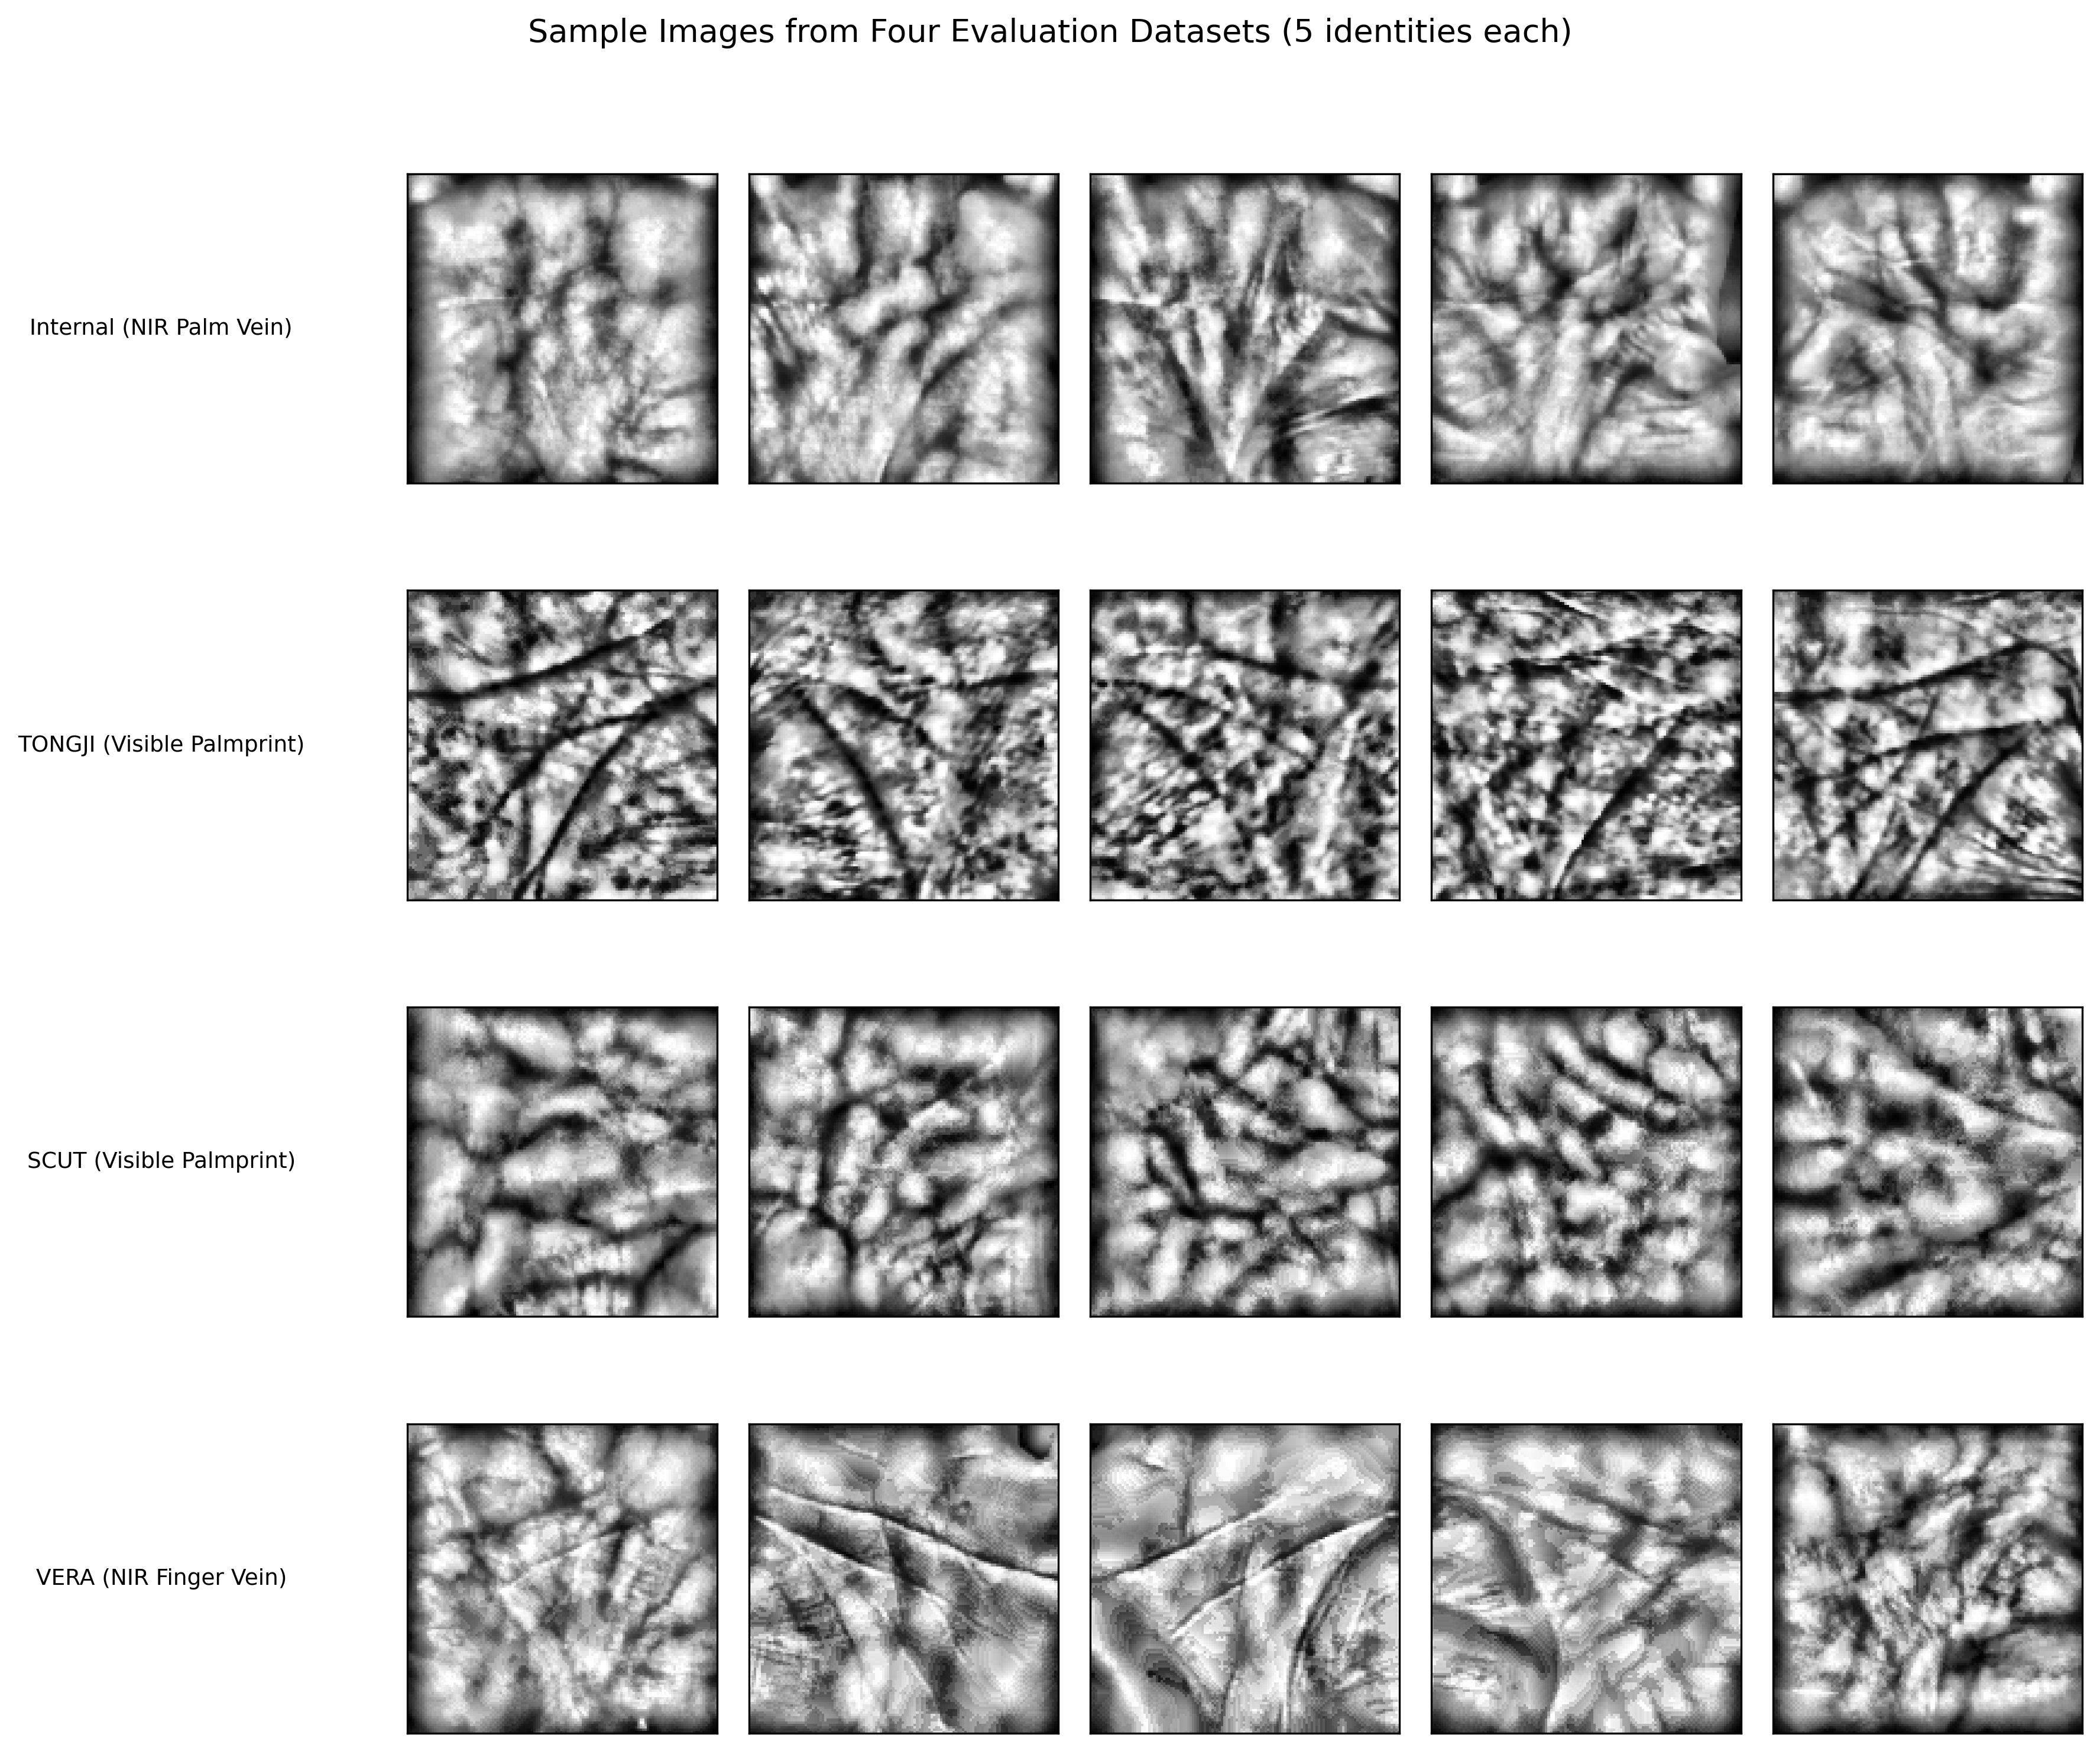
\includegraphics[width=\textwidth]{fig_dataset_samples.png}}
\caption{Ảnh mẫu đại diện từ bốn bộ dữ liệu thực nghiệm, minh họa sự đa dạng về phương thức thu nhận (NIR vs. Visible) và đặc trưng kết cấu mạch máu/vân da.}
\label{fig:dataset_samples}
\end{figure}

%% ====== SECTION IV ======
\section{Phương pháp Đề xuất}

\subsection{Phát biểu Bài toán}

Nghiên cứu này tập trung vào bài toán xác thực tĩnh mạch lòng bàn tay không tiếp xúc trong điều kiện giao thức open-set. Cho hai ảnh tĩnh mạch, mục tiêu là xác định liệu chúng có thuộc cùng một danh tính hay không (xác thực 1:1). Mỗi ảnh đầu vào được ánh xạ vào một vector đặc trưng gọn nhẹ (\textit{embedding}) trong một không gian metric. Quá trình xác thực được thực hiện bằng cách tính toán độ tương đồng giữa hai embedding và so sánh với một ngưỡng quyết định.

\begin{figure}[H]
\centerline{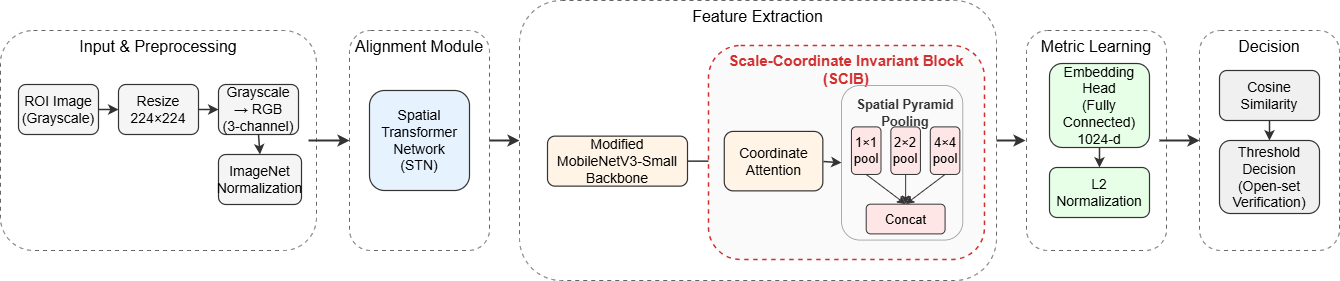
\includegraphics[width=\columnwidth]{fig_framework.png}}
\caption{Kiến trúc của khung xác thực tĩnh mạch lòng bàn tay theo giao thức open-set.}
\label{fig:framework}
\end{figure}

\subsection{Tiền xử lý và Chuẩn hóa Đầu vào}

Quy trình tiền xử lý bao gồm ba giai đoạn chính: phân đoạn vùng lòng bàn tay, chuẩn hóa tỷ lệ hình học và tăng cường quang học.

Việc trích xuất vùng quan tâm (ROI) được thực hiện theo hai phương thức tùy thuộc vào nguồn dữ liệu:

\begin{itemize}
    \item \textbf{Phương thức 1 (Mặc định):} Khi thiết bị thu nhận cung cấp tọa độ ROI (4 điểm góc polygon), phép biến đổi phối cảnh (\textit{Perspective Transform}) được áp dụng trực tiếp để crop và chuẩn hóa vùng ROI về kích thước $128 \times 128$ pixel.
    \item \textbf{Phương thức 2 (Dự phòng):} Khi không có tọa độ ROI có sẵn, pipeline tự động phân đoạn bằng GrabCut kết hợp phép biến đổi khoảng cách (Distance Transform) được sử dụng để xác định tâm lòng bàn tay và trích xuất ROI.
\end{itemize}

\begin{figure}[H]
\centerline{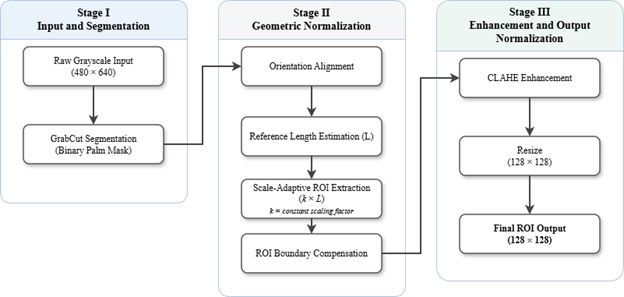
\includegraphics[width=\columnwidth]{fig_preprocessing.png}}
\caption{Quy trình tiền xử lý ba giai đoạn cho trích xuất và chuẩn hóa vùng quan tâm (ROI).}
\label{fig:preprocessing}
\end{figure}

\subsubsection{Phân đoạn Lòng bàn tay}

\begin{figure}[H]
\centerline{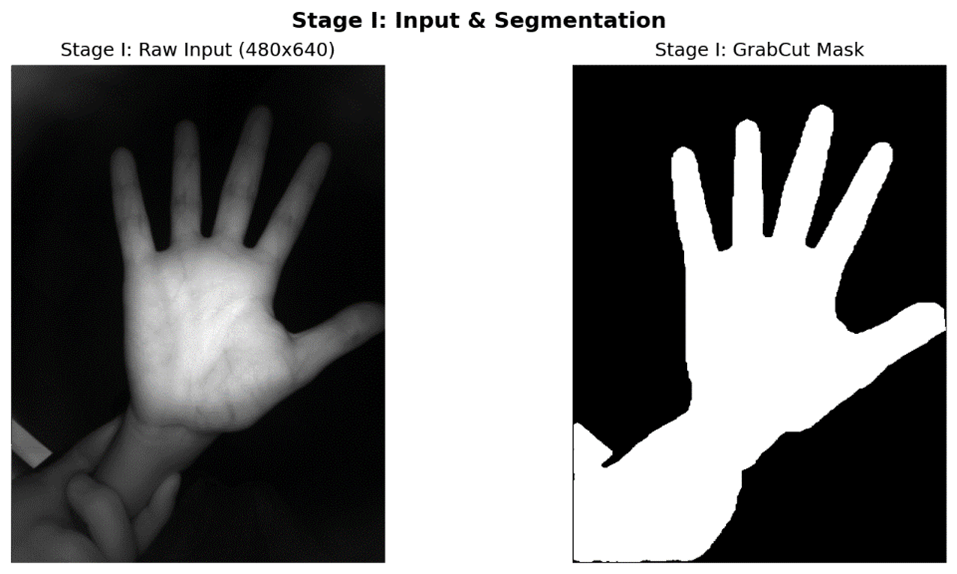
\includegraphics[width=\columnwidth]{fig_segmentation.png}}
\caption{Giai đoạn thứ nhất xử lý ảnh nguyên thủy và phân đoạn vùng bàn tay.}
\label{fig:segmentation}
\end{figure}

Cho ảnh đầu vào thang xám $I \in \mathbb{R}^{H \times W}$, thuật toán GrabCut tự động được áp dụng với khởi tạo hộp bao (\textit{bounding box}) bao phủ toàn bộ ảnh. Quá trình phân đoạn tạo ra một mặt nạ nhị phân $M(x,y) \in \{0,1\}$, trong đó các điểm ảnh tiền cảnh tương ứng với vùng lòng bàn tay. Mặt nạ này sau đó được sử dụng cho phân tích hình học và bước trích xuất vùng quan tâm (ROI).

\subsubsection{Chuẩn hóa Tỷ lệ Hình học}

\begin{figure}[H]
\centerline{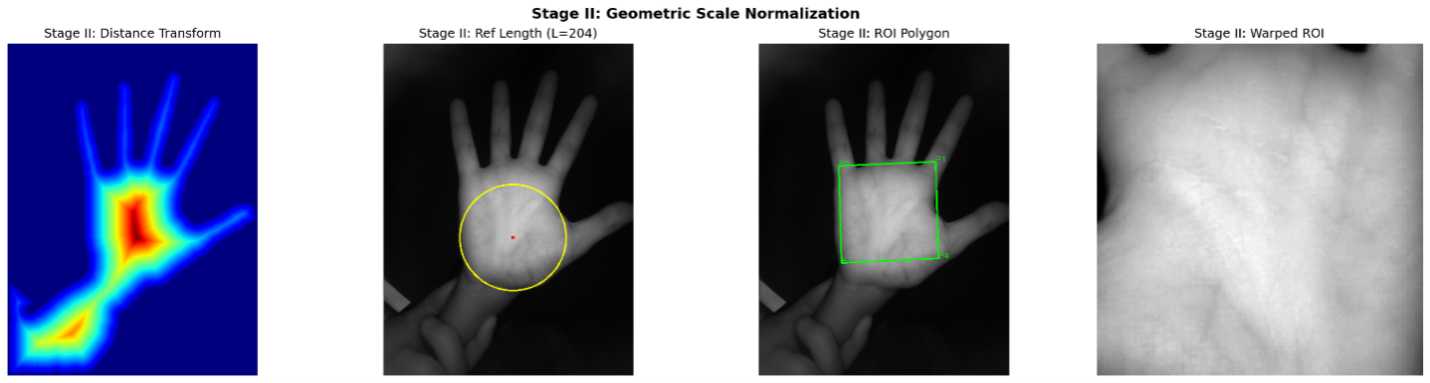
\includegraphics[width=\columnwidth]{fig_scale_norm.png}}
\caption{Giai đoạn thứ hai chuẩn hóa thang đo hình học.}
\label{fig:scale_norm}
\end{figure}

Phép biến đổi khoảng cách Euclid được tính:
\begin{equation}
D(x,y) = \min_{(u,v) \in \partial M} \sqrt{(x-u)^2 + (y-v)^2}
\label{eq:dt}
\end{equation}
trong đó $\partial M$ biểu diễn biên của vùng lòng bàn tay. Độ dài tham chiếu nội tại $L$ được định nghĩa:
\begin{equation}
L = \max_{(x,y) \in M} D(x,y)
\label{eq:ref_length}
\end{equation}
Tọa độ tâm tương ứng:
\begin{equation}
(x_c, y_c) = \arg\max_{(x,y) \in M} D(x,y)
\label{eq:center}
\end{equation}
Vùng quan tâm hình vuông (ROI) được trích xuất với kích thước $\text{ROI size} = k \cdot L$, trong đó $k$ là hằng số tỷ lệ cố định:
\begin{equation}
\text{ROI} = I\left[x_c - \frac{kL}{2} : x_c + \frac{kL}{2},\; y_c - \frac{kL}{2} : y_c + \frac{kL}{2}\right]
\label{eq:roi}
\end{equation}

\subsubsection{Tăng cường Quang học và Định dạng Dữ liệu}

\begin{figure}[H]
\centerline{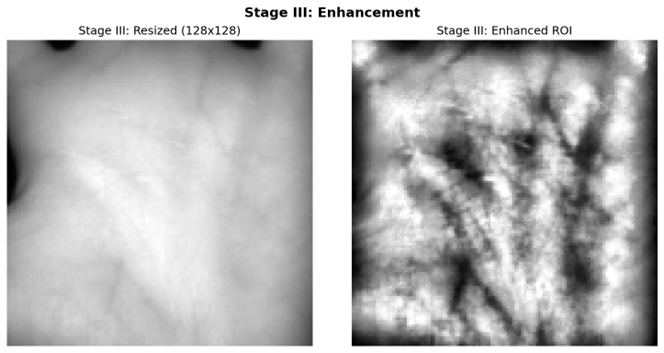
\includegraphics[width=\columnwidth]{fig_clahe.png}}
\caption{Giai đoạn thứ ba: Tăng cường độ tương phản cục bộ bằng CLAHE.}
\label{fig:clahe}
\end{figure}

Sau khi vùng ROI được trích xuất, thuật toán CLAHE (\textit{Contrast Limited Adaptive Histogram Equalization}) được áp dụng độc lập trên từng ảnh ở kích thước $128\times 128$ pixel. Xử lý ở cấp độ ảnh đơn lẻ đảm bảo không sử dụng thông tin thống kê toàn cục, loại trừ nguy cơ rò rỉ dữ liệu (\textit{data leakage}) trước khi chia tập. Ảnh sau đó được resize về $224\times 224$ pixel, nhân bản thành 3 kênh, và chuẩn hóa Z-score theo hằng số ImageNet ($\mu = [0.485, 0.456, 0.406]$, $\sigma = [0.229, 0.224, 0.225]$).

Pipeline tăng cường dữ liệu (\textit{data augmentation}) được áp dụng on-the-fly trên tập huấn luyện qua \texttt{BiometricCompose}, bao gồm:
\begin{itemize}
    \item \textbf{Biến đổi hình học:} Xoay ngẫu nhiên $\pm 12^\circ$ ($p=0.8$), dịch chuyển tịnh tiến $\pm 12\%$ kích thước ảnh ($p=0.8$), co giãn $\pm 8\%$ ($p=0.6$).
    \item \textbf{Biến đổi quang học:} Nhiễu Gaussian $\mathcal{N}(0, 0.025^2)$ ($p=0.6$), hệ số tương phản $[0.75, 1.25]$ ($p=0.7$), độ sáng $[0.88, 1.12]$ ($p=0.7$).
\end{itemize}

Pipeline tăng cường được áp dụng đồng nhất cho tất cả 12 kiến trúc trên 4 bộ dữ liệu. Tập kiểm thử không qua bất kỳ augmentation nào.

\begin{figure}[H]
\centerline{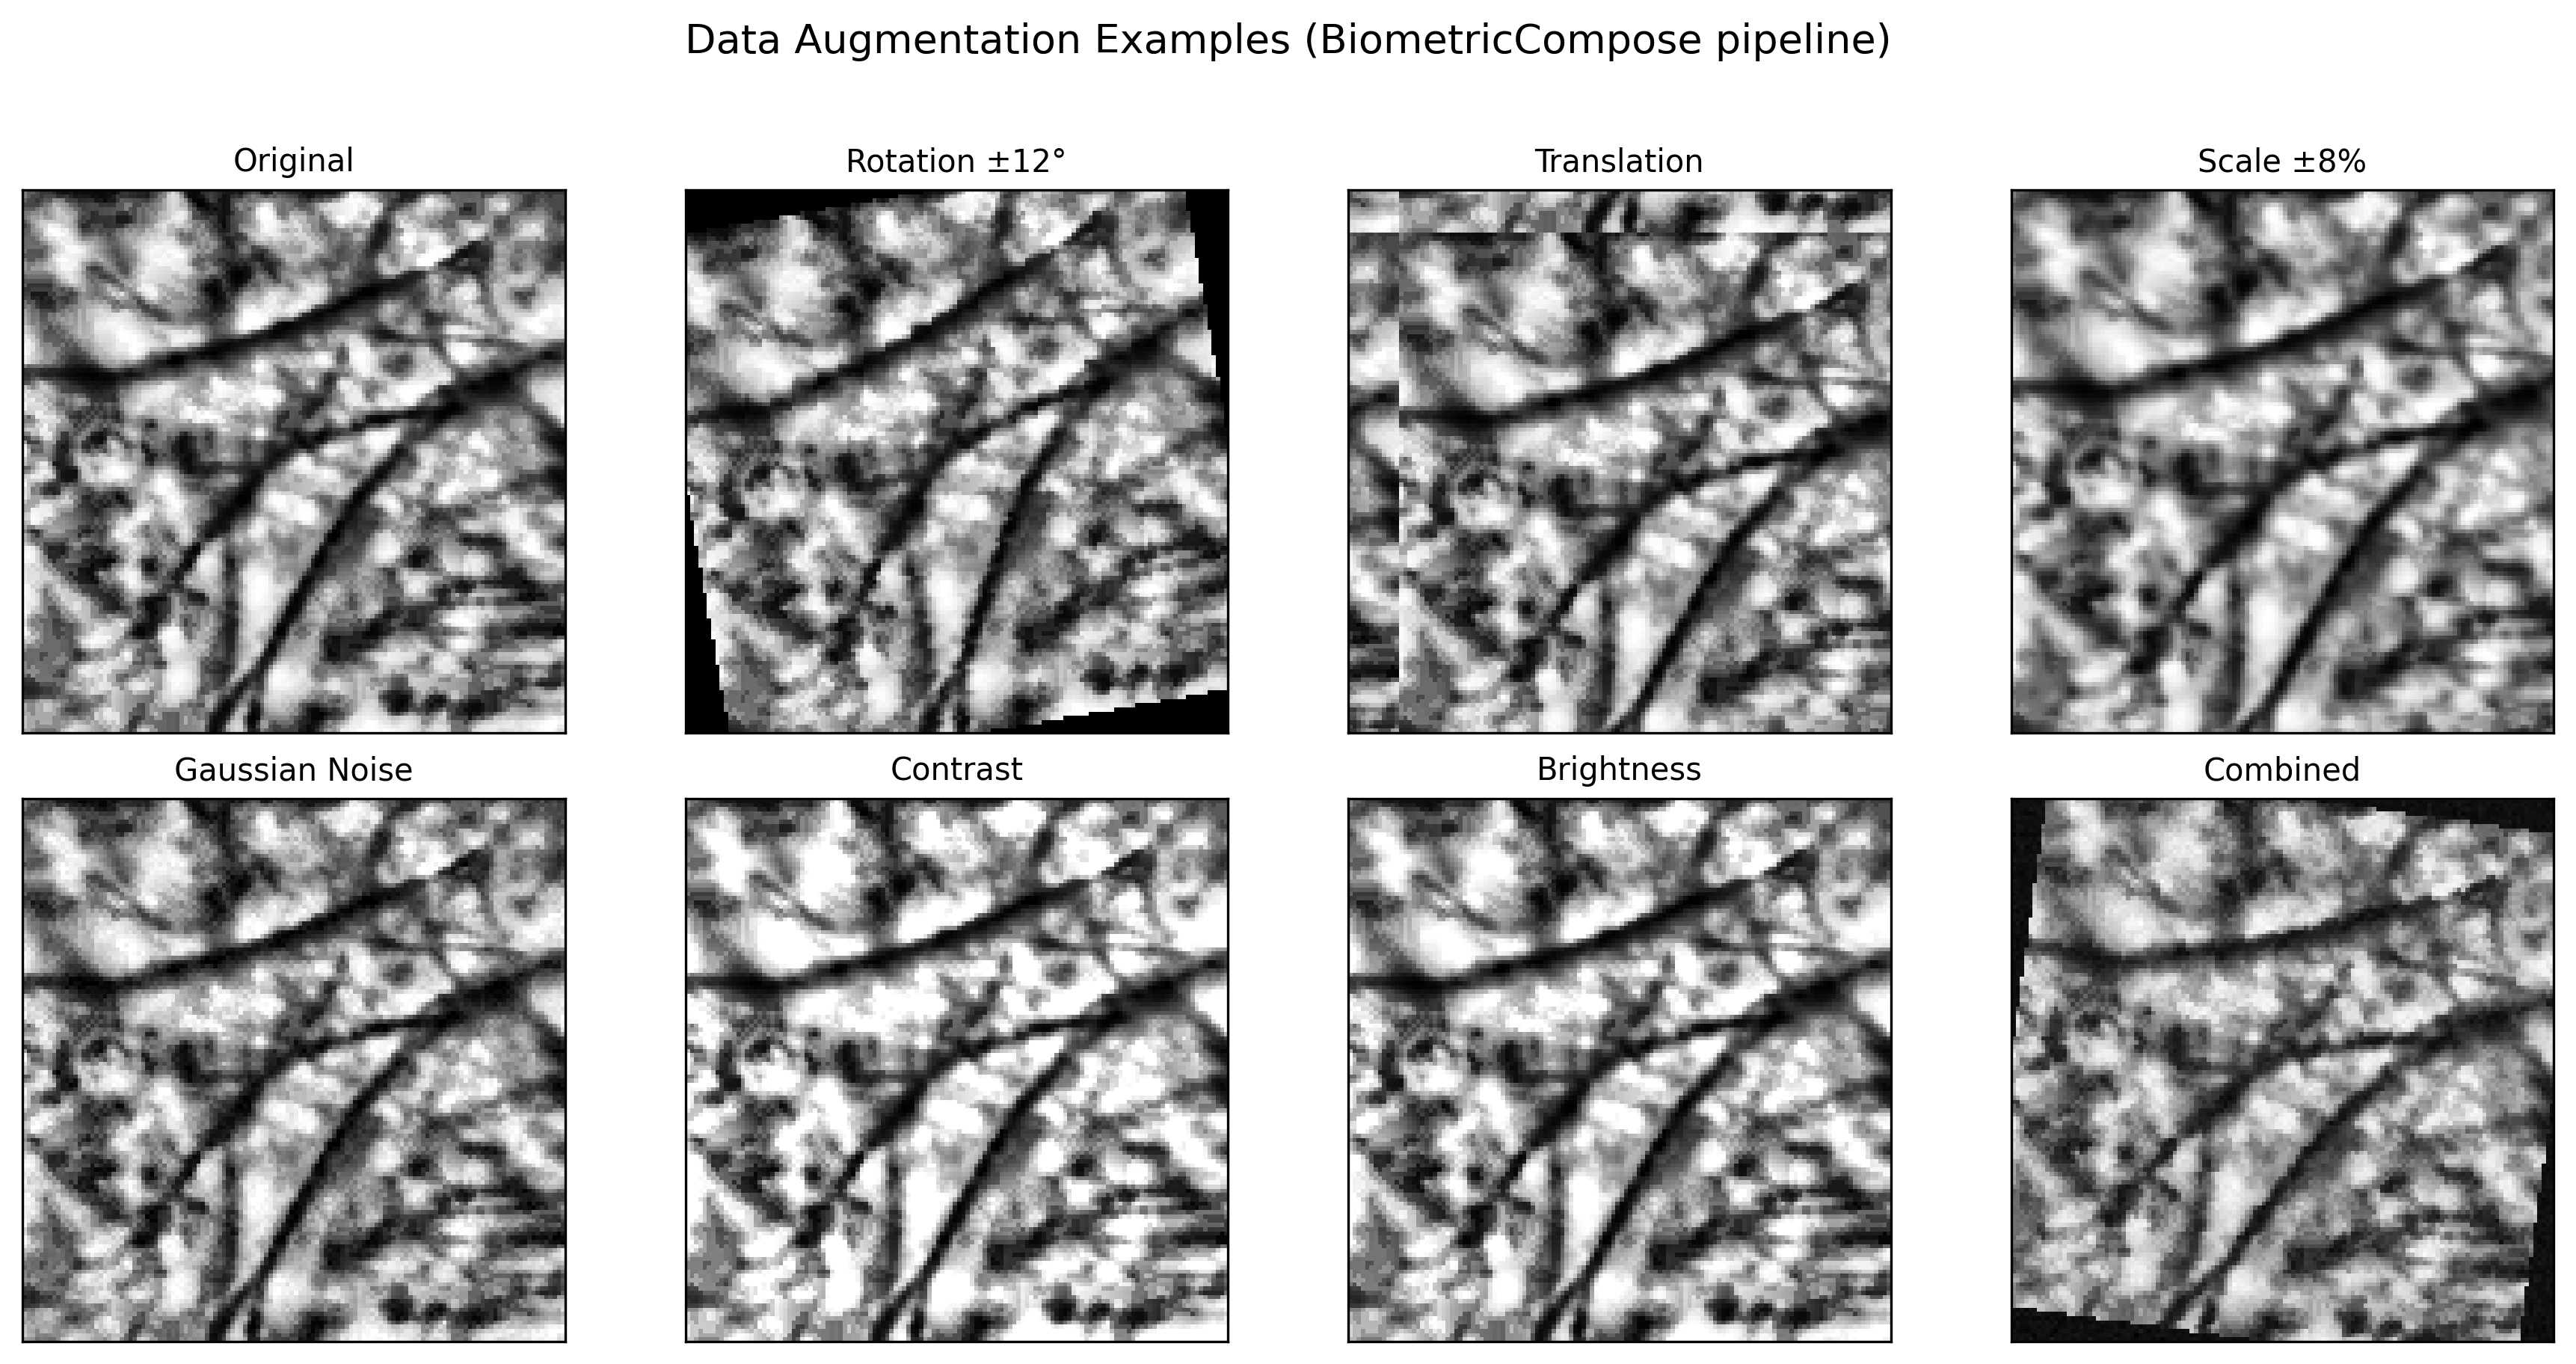
\includegraphics[width=\textwidth]{fig_augmentation_examples.png}}
\caption{Minh họa các phép tăng cường dữ liệu on-the-fly trên tập huấn luyện. Hàng trên: ảnh gốc; các cột: biến đổi hình học (xoay, dịch, co giãn) và quang học (nhiễu, tương phản, độ sáng).}
\label{fig:augmentation}
\end{figure}

\subsection{Kiến trúc Đề xuất SCA-MobileNet}

SCA-MobileNet được thiết kế như một kiến trúc thống nhất cho bài toán xác thực tĩnh mạch lòng bàn tay. Thay vì ghép nối rời rạc các module vào backbone, kiến trúc tích hợp khối \textbf{Scale-Coordinate Invariant Block (SCIB)} trực tiếp vào luồng trích xuất đặc trưng.

Mạng xương sống MobileNetV3-Small \cite{b10} được sử dụng với trọng số khởi tạo từ ImageNet. Do đặc trưng nhận dạng của tĩnh mạch tập trung ở mức chi tiết cục bộ (điểm nối, rẽ nhánh) thay vì ngữ nghĩa cấp cao, hai lớp cuối (lớp 10 và 11) của backbone gốc được loại bỏ. Đặc trưng từ backbone rút gọn này được đưa vào khối SCIB để tạo biểu diễn bất biến tỷ lệ. Tại đầu vào, mạng chuyển đổi không gian STN \cite{b9} chuẩn hóa hình học; tại đầu ra, hàm mất mát AdaCos \cite{b11} tối ưu hóa không gian embedding.

\subsubsection{Spatial Transformer Network (STN)}
Để xử lý sai lệch hình học trong quá trình thu nhận không tiếp xúc, SCA-MobileNet tích hợp mô-đun STN \cite{b9} tại đầu vào. Mạng định vị (\textit{Localization Network}) bao gồm các lớp tích chập, Max Pooling và Adaptive Average Pooling ($4 \times 4$), tiếp nối bởi các lớp kết nối đầy đủ để hồi quy tham số biến đổi Affine 2D.

Kết quả của mạng định vị là ma trận $\theta \in \mathbb{R}^{2\times3}$ chứa 6 tham số cho phép xoay, tịnh tiến và co giãn. Quan hệ tọa độ giữa điểm đích $(x_i^t, y_i^t)$ và điểm nguồn $(x_i^s, y_i^s)$:
\begin{equation}
\begin{pmatrix} x_i^s \\ y_i^s \end{pmatrix} = \mathcal{T}_\theta(G_i) = \begin{pmatrix} \theta_{11} & \theta_{12} & \theta_{13} \\ \theta_{21} & \theta_{22} & \theta_{23} \end{pmatrix} \begin{pmatrix} x_i^t \\ y_i^t \\ 1 \end{pmatrix}
\label{eq:stn}
\end{equation}
Ảnh đầu ra $V$ được tái tạo qua nội suy song tuyến tính (\textit{bilinear interpolation}) trên lưới tọa độ đã biến đổi, cung cấp tính bất biến không gian cho các tầng trích xuất đặc trưng phía sau.

\subsection{Khối SCIB (Scale-Coordinate Invariant Block)}

Trong CNN truyền thống, tầng Global Average Pooling (GAP) cuối cùng nén bản đồ đặc trưng $H \times W \times C$ thành vector $1 \times 1 \times C$, loại bỏ toàn bộ thông tin vị trí không gian. Đối với bài toán nhận dạng tĩnh mạch --- nơi cấu trúc hình học (điểm nối, rẽ nhánh) mang tính phân biệt cao --- việc mất thông tin tọa độ làm giảm khả năng phân biệt của embedding. SCIB giải quyết hạn chế này bằng hai giai đoạn tuần tự.

\textbf{Giai đoạn 1 --- Mã hóa tọa độ (Coordinate Attention):} SCIB áp dụng cơ chế phân rã tọa độ 1D (Coordinate Attention) \cite{b7}. Cho đầu vào $\mathbf{X} \in \mathbb{R}^{C \times H \times W}$, phép gộp tọa độ sử dụng hai bộ lọc kích thước $(H, 1)$ và $(1, W)$ để chiếu $\mathbf{X}$ theo từng trục.
Đối với kênh thứ $c$ ở chiều cao $h$:
\begin{equation}
z_c^h(h) = \frac{1}{W}\sum_{0 \le j < W} \mathbf{X}_c(h, j)
\end{equation}
Đối với kênh thứ $c$ ở chiều rộng $w$:
\begin{equation}
z_c^w(w) = \frac{1}{H}\sum_{0 \le i < H} \mathbf{X}_c(i, w)
\end{equation}
Hai chuỗi vector này được nối (concatenate) và mã hóa phi tuyến qua một lớp chập, sau đó tách thành hai trọng số kích hoạt sigmoid:
\begin{equation}
y_c(i,j) = x_c(i,j) \times g_c^h(i) \times g_c^w(j)
\label{eq:ca}
\end{equation}
Phép nhân Hadamard tại (\ref{eq:ca}) cho phép mạng tăng cường các vùng có cấu trúc tĩnh mạch theo cả hai trục không gian.

\textbf{Giai đoạn 2 --- Gộp kim tự tháp không gian (Spatial Pyramid Pooling):} Bản đồ đặc trưng $\mathbf{F}_{\text{CA}} \in \mathbb{R}^{C \times H_{out} \times W_{out}}$ sau bước CA được đưa vào SPP \cite{b8} với $n=3$ cấp lưới $\{1\times1, 2\times2, 4\times4\}$. Tại mỗi cấp $k \times k$, cửa sổ gộp và sải bước được tính động:
\begin{equation}
V_{\text{SCIB}} = \left[ \mathop{\oplus}_{pool \in \{1,2,4\}} \text{MaxPool}_{pool\times pool} \left( \mathbf{F}_{\text{CA}} \right) \right]
\label{eq:spp}
\end{equation}
Toán tử concatenate $\oplus$ tạo biểu diễn có độ dài cố định $C \cdot (1^2 + 2^2 + 4^2) = 21C$. Trình tự CA $\rightarrow$ SPP đảm bảo embedding vừa bảo toàn thông tin tọa độ của cấu trúc tĩnh mạch, vừa bất biến với thay đổi tỷ lệ đầu vào.

\begin{figure}[H]
\centerline{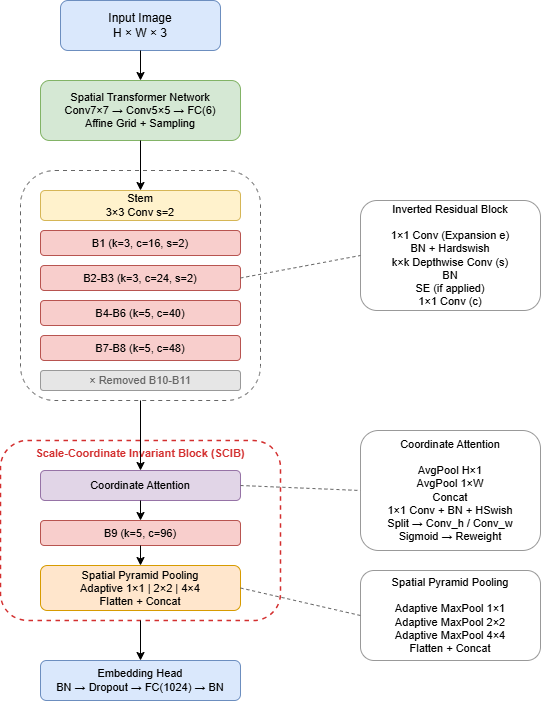
\includegraphics[width=\columnwidth]{fig_architecture.png}}
\caption{Kiến trúc tổng thể của SCA-MobileNet. Khối SCIB (CA + SPP) tạo biểu diễn đặc trưng bảo toàn thông tin hình học.}
\label{fig:architecture}
\end{figure}

\subsubsection{Luồng dữ liệu tổng thể}
Ảnh đầu vào $I$ qua STN để chuẩn hóa hình học thành $I_{\text{aligned}}$. Backbone MobileNetV3-Small rút gọn trích xuất bản đồ đặc trưng $F \in \mathbb{R}^{C \times H' \times W'}$. Khối SCIB tạo vector bất biến $V_{\text{SCIB}}$. Cuối cùng, Embedder ($E$) gồm Batch Normalization 1D, Dropout và Linear Projection chiếu vector này thành embedding $v_{\text{final}} \in \mathbb{R}^{1024}$ cho hàm mất mát AdaCos. Toàn bộ kiến trúc được tối ưu end-to-end.



\subsection{Hàm mất mát AdaCos}

Mục tiêu của mô hình là học không gian embedding trong đó khoảng cách nội lớp (\textit{intra-class}) được tối thiểu hóa và khoảng cách liên lớp (\textit{inter-class}) được tối đa hóa. Hàm Softmax truyền thống không áp đặt ràng buộc hình học lên embedding, dẫn đến ranh giới quyết định thiếu chặt chẽ. Các phương pháp angular margin như SphereFace \cite{b16}, CosFace \cite{b15} và ArcFace \cite{b14} cải thiện điều này nhưng đòi hỏi điều chỉnh siêu tham số $(s, m)$ theo từng bộ dữ liệu.

Nghiên cứu sử dụng biến thể của hàm mất mát AdaCos \cite{b11} với tham số tỷ lệ tự động:
\begin{equation}
s = \sqrt{2} \cdot \log(C - 1)
\label{eq:scale}
\end{equation}
trong đó $C$ là số lượng định danh huấn luyện. Khác với AdaCos gốc (chỉ sử dụng $s$ tự động mà không áp biên góc), nghiên cứu bổ sung biên góc cộng cố định $m = 0.35$ (\textit{Additive Angular Margin}, tương tự ArcFace \cite{b14}) để tăng cường phân tách liên lớp. Hàm mất mát cho mẫu $i$ thuộc lớp $y_i$:
\begin{equation}
\mathcal{L} = -\log \frac{e^{s \cdot (\cos(\theta_{i,y_i}) - m)}}{e^{s \cdot (\cos(\theta_{i,y_i}) - m)} + \sum_{k \neq y_i} e^{s \cdot \cos(\theta_{i,k})}}
\label{eq:loss}
\end{equation}
trong đó $\cos(\theta_{i,y_i}) - m$ là cosine của lớp đúng đã trừ biên $m$, và $s$ là hệ số tỷ lệ tự động. Việc tính tự động $s$ theo AdaCos cho phép mô hình hoạt động ổn định trên các bộ dữ liệu có quy mô khác nhau mà không cần điều chỉnh thủ công, trong khi biên $m$ tăng cường tính gom tụ nội lớp trên mặt siêu cầu cho tác vụ open-set verification.


%% ====== SECTION V ======
\section{Kết quả Thực nghiệm}

\subsection{Giao thức Đánh giá}

Tất cả thực nghiệm sử dụng giao thức xác thực open-set \cite{b13}: tập kiểm thử chứa các định danh không xuất hiện trong quá trình huấn luyện. Chia tập theo tỷ lệ 70:30 (\textit{random seed}~=~42) \textbf{ở cấp độ danh tính} (\textit{identity-level split}), đảm bảo không trùng lặp (disjoint-identity) giữa tập huấn luyện và kiểm thử.

\textbf{Bộ dữ liệu tự thu thập (1.549 định danh):} Phân chia thành 1.084 định danh huấn luyện (10.840 ảnh) và 465 định danh kiểm thử (4.650 ảnh). Số cặp genuine được sinh theo tổ hợp: $\binom{10}{2} \times 465 = 20.925$ cặp. Số cặp impostor được lấy mẫu ngẫu nhiên cân bằng, tạo tổng cộng \textbf{41.850 phép so khớp}.

\textbf{Bộ dữ liệu TONGJI (1.200 định danh):} Phân chia thành 840 định danh huấn luyện (8.400 ảnh) và 360 định danh kiểm thử (3.600 ảnh). Tương tự, $\binom{10}{2} \times 360 = 16.200$ cặp genuine và 16.200 cặp impostor, tổng cộng \textbf{32.400 phép so khớp}.

\textbf{Bộ dữ liệu SCUT FVP (1.100 định danh):} Phân chia thành 770 định danh huấn luyện (7.700 ảnh) và 330 định danh kiểm thử (3.300 ảnh). Số cặp: $\binom{10}{2} \times 330 = 14.850$ cặp genuine và 14.850 cặp impostor, tổng cộng \textbf{29.700 phép so khớp}.

\textbf{Bộ dữ liệu VERA (220 định danh):} Phân chia thành 154 định danh huấn luyện (770 ảnh) và 66 định danh kiểm thử (330 ảnh). Với chỉ 5 mẫu/ID: $\binom{5}{2} \times 66 = 660$ cặp genuine và 660 cặp impostor, tổng cộng \textbf{1.320 phép so khớp}. Đây là bộ dữ liệu có quy mô nhỏ nhất, hạn chế độ phân giải thống kê của các chỉ số TAR tại FAR thấp.

\textbf{Nguyên tắc thực nghiệm:} Tất cả \textbf{12 mô hình} được huấn luyện \textbf{độc lập từ đầu} trên \textbf{từng bộ dữ liệu} với cùng giao thức chia tập, random seed, và pipeline tăng cường dữ liệu. Không có mô hình nào tái sử dụng trọng số từ thực nghiệm trên bộ dữ liệu khác (ngoại trừ thí nghiệm cross-domain riêng).

\textbf{Tiền xử lý theo đặc thù bộ dữ liệu:} Bộ dữ liệu nội bộ yêu cầu pipeline đầy đủ: phân đoạn GrabCut $\rightarrow$ trích xuất ROI + chuẩn hóa tỷ lệ $\rightarrow$ CLAHE. Ba bộ dữ liệu công khai (TONGJI, SCUT, VERA) đã cung cấp sẵn ROI, chỉ cần CLAHE và chuẩn hóa kích thước. Tất cả ảnh đầu vào cuối cùng có kích thước $224 \times 224 \times 3$ (FGFNet: $256 \times 256 \times 3$) với chuẩn hóa Z-score theo hằng số ImageNet.

Cần lưu ý rằng số lượng cặp impostor ảnh hưởng trực tiếp đến độ phân giải của chỉ số TAR tại các ngưỡng FAR rất thấp. Với 16.200 cặp impostor trên TONGJI, tại FAR~=~0,01\% chỉ cho phép tối đa $\lfloor 16.200 \times 0,0001 \rfloor \approx 1{-}2$ cặp bị chấp nhận sai. Trên VERA, con số này chỉ là $\lfloor 660 \times 0,0001 \rfloor < 1$, do đó chỉ số TAR@0,01\% trên VERA cần được diễn giải thận trọng. Để cung cấp góc nhìn toàn diện và nhất quán, chúng tôi báo cáo đầy đủ cả hai chỉ số TAR@0,01\% và TAR@0,1\% trên tất cả các kịch bản kiểm thử.

Equal Error Rate (EER) là chỉ số chính. True Acceptance Rate (TAR) được báo cáo tại FAR = 0,01\%, 0,1\% và 1\%. Area Under Curve (AUC) của đường cong ROC được tính như chỉ số tổng hợp.

\begin{figure}[H]
\centerline{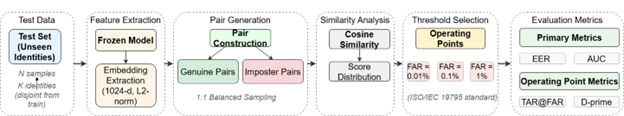
\includegraphics[width=\columnwidth]{fig_evaluation_pipeline.png}}
\caption{Pipeline đánh giá xác thực open-set bao gồm trích xuất embedding, sinh cặp cân bằng, phân tích độ tương đồng, lựa chọn ngưỡng và tính toán các chỉ số tuân theo tiêu chuẩn ISO \cite{b17}.}
\label{fig:eval_pipeline}
\end{figure}

\subsection{Cấu hình Mạng lưới và Tối ưu hóa Thực nghiệm (Reproducibility Protocol)}

Chi tiết cấu hình mạng được trình bày để đảm bảo tính tái lập (\textit{reproducibility}). Backbone MobileNetV3-Small sử dụng trọng số pretrained từ ImageNet \cite{b10}, cắt bỏ hai lớp cuối (\texttt{return\_layers=\{'9': 'out'\}}). STN được khởi tạo từ ma trận đồng nhất:
\begin{equation}
\theta_{init} = \begin{bmatrix} 1 & 0 & 0 \\ 0 & 1 & 0 \end{bmatrix}
\end{equation}
Trọng số lớp chập cuối của STN được khởi tạo zero (\texttt{nn.init.zeros\_}) để STN hoạt động như phép đồng nhất trong các epoch đầu, tránh biến dạng ảnh trước khi gradient ổn định.

Đầu ra mạng là vector embedding 1024 chiều. Hàm mất mát \texttt{AdaCos} sử dụng lề $m=0.35$ và hệ số tỷ lệ $s = \sqrt{2} \cdot \log(C-1)$, với $C$ là số định danh huấn luyện. Giá trị $s$ thay đổi theo bộ dữ liệu: $s \approx 9.89$ (Nội bộ, $C=1.084$), $s \approx 9.53$ (TONGJI, $C=840$), $s \approx 9.40$ (SCUT, $C=770$), và $s \approx 7.13$ (VERA, $C=154$). Bộ gom lô \texttt{BalancedBatchSampler} chọn 16 định danh, mỗi định danh 4 mẫu (batch size = 64), đảm bảo đa dạng mini-batch cho AdaCos. Tối ưu hóa bằng \texttt{AdamW} ($\alpha=0.001$, $\beta_1=0.9$, $\beta_2=0.999$).

Huấn luyện gồm hai giai đoạn: trong 5 epoch đầu (warm-up), backbone bị đóng băng, chỉ huấn luyện CA, Embedder và AdaCos. Từ epoch 6 trở đi, toàn bộ tham số được cập nhật. Tổng cộng 100 epoch. \texttt{Automatic Mixed Precision (AMP - fp16)} được sử dụng để tăng thông lượng, kết hợp \texttt{Gradient Clipping} ($max\_norm = 10.0$) để ổn định gradient của STN.

Thực nghiệm chạy trên GPU \texttt{NVIDIA RTX 4050 Laptop 6GB VRAM}. Thời gian suy luận đo được 10,01~ms/ảnh trên GPU (99,9 FPS). Kiến trúc có 3,19M tham số và 0,13G FLOPs, phù hợp triển khai trên thiết bị biên (\textit{edge devices}).

\subsubsection{Tổng hợp Kiến trúc Mô hình Thực nghiệm}

Để thiết lập so sánh toàn diện, chúng tôi đánh giá SCA-MobileNet cùng 11 kiến trúc baseline, bao gồm cả các phương pháp sinh trắc chuyên dụng và các backbone tổng quát. Bảng~\ref{tab:model_architectures} mô tả chi tiết từng mô hình.

\begin{table}[H]
\caption{Tổng hợp 12 kiến trúc mô hình được đánh giá. Params và FLOPs đo ở đầu vào $224\times224\times3$ (FGFNet: $256\times256\times3$).}
\begin{center}
\resizebox{\textwidth}{!}{%
\begin{tabular}{l|l|l|c|c|c|l}
\hline
\textbf{Mô hình} & \textbf{Backbone} & \textbf{Thiết kế chính} & \textbf{Params (M)} & \textbf{FLOPs (G)} & \textbf{Emb. Dim} & \textbf{Nguồn} \\
\hline
\textbf{SCA-MobileNet (Ours)} & MobileNetV3-Small & STN + CA + SPP (SCIB) & 3.19 & 0.13 & 1024 & Đề xuất \\
MobileNetV3 (Base) & MobileNetV3-Small & Chỉ backbone (GAP) & 1.52 & 0.06 & 1024 & \cite{b10} \\
EfficientNet-B0 & EfficientNet-B0 & MBConv + SE & 4.01 & 0.38 & 1024 & \cite{b20} \\
ResNet50 & ResNet-50 & Residual blocks + GSCL head & 23.51 & 4.13 & 1024 & \cite{b3} \\
Swin-Tiny & Swin Transformer & Shifted window attention & 27.52 & 4.37 & 1024 & --- \\
DeiT-Tiny & DeiT Transformer & ViT + distillation token & 5.52 & 1.07 & 1024 & --- \\
MobileViT-S & MobileViT-Small & MobileNet + ViT hybrid & 4.94 & 1.83 & 1024 & --- \\
MPSNet & Multi-path CNN & SPP $[1,2,4]$ + đa nhánh & 2.99 & 0.14 & 1024 & \cite{b1} \\
Modified-DenseNet161 & DenseNet-161 & Dense connections & 28.74 & 7.95 & 1024 & \cite{b2} \\
GSCL & ResNet-18 & Contrastive + CosFace & 11.23 & 1.82 & 512 & \cite{b3} \\
RSNet & Dual-branch CNN & Local RLEB + Global MAB & 6.23 & 1.17 & 1024 & \cite{b4} \\
FGFNet & MobileViT + FFC & FFT spatial attention & 5.62 & 6.37 & 640 & \cite{b5} \\
\hline
\end{tabular}%
}
\label{tab:model_architectures}
\end{center}
\end{table}

\subsubsection{Chi tiết Cấu hình Huấn luyện cho từng Kiến trúc}

Bảng~\ref{tab:training_config} trình bày chi tiết cấu hình huấn luyện được áp dụng nhất quán cho tất cả các thí nghiệm. Mọi mô hình được huấn luyện với cùng giao thức cơ bản nhằm đảm bảo tính so sánh công bằng.

\begin{table}[H]
\caption{Cấu hình huấn luyện chi tiết. Tất cả mô hình sử dụng cùng giao thức cơ bản trừ các tham số đặc thù kiến trúc.}
\begin{center}
\resizebox{\textwidth}{!}{%
\begin{tabular}{l|l}
\hline
\textbf{Tham số} & \textbf{Giá trị} \\
\hline
\multicolumn{2}{|c|}{\textbf{Cấu hình chung (Tất cả mô hình)}} \\
\hline
Input size & $224 \times 224 \times 3$ (FGFNet: $256 \times 256 \times 3$) \\
Epochs & 100 (full training, không early stopping) \\
Evaluation frequency & Mỗi 5 epochs \\
Random seed & 42 \\
Mixed precision & AMP (fp16) \\
Gradient clipping & $max\_norm = 10.0$ \\
Hardware & NVIDIA RTX 4050 Laptop 6GB VRAM \\
Framework & PyTorch 2.0+ \\
\hline
\multicolumn{2}{|c|}{\textbf{SCA-MobileNet (Đề xuất)}} \\
\hline
Loss function & AdaCos ($s = \sqrt{2} \cdot \log(C-1)$, $m = 0.35$) + CrossEntropy (label\_smoothing=0.1) \\
Optimizer & AdamW ($\beta_1=0.9$, $\beta_2=0.999$, weight\_decay=$10^{-4}$) \\
Learning rate & $\alpha = 0.001$ \\
Scheduler & MultiStepLR (milestones: [30, 60, 85], $\gamma=0.1$) \\
Batch sampler & BalancedBatchSampler (16 classes $\times$ 4 samples = 64/batch) \\
Warmup & 5 epochs (backbone frozen, chỉ train CA + Embedder + AdaCos) \\
Feature dimension & 1024 \\
Dropout & 0.3 \\
Backbone init & ImageNet pretrained, cắt layer 10--11 (\texttt{return\_layers=\{'9':'out'\}}) \\
STN init & Ma trận đồng nhất ($\theta = I_{2\times3}$), trọng số zero-init \\
\hline
\multicolumn{2}{|c|}{\textbf{Backbone thay thế (EfficientNet-B0, Swin-Tiny, DeiT-Tiny, MobileViT-S)}} \\
\hline
Loss function & AdaCos (giống SCA-MobileNet) \\
Optimizer & AdamW (layer-wise LR decay) \\
Learning rate & Base LR = $5 \times 10^{-5}$, LR decay = 0.65 \\
Scheduler & CosineAnnealingLR ($T_{max} = 95$, $\eta_{min} = 10^{-7}$) \\
Warmup & 5 epochs (backbone frozen) \\
\hline
\multicolumn{2}{|c|}{\textbf{MobileNetV3 (Base) --- Ablation baseline}} \\
\hline
Loss function & AdaCos (giống SCA-MobileNet, không STN/CA/SPP) \\
Optimizer/Scheduler & Giống SCA-MobileNet \\
\hline
\multicolumn{2}{|c|}{\textbf{RSNet}} \\
\hline
Loss function & AdaFace (scale=50, margin=0.55, $h$=0.29) + DifferenceLoss \\
Optimizer & Adam ($\alpha=0.001$) \\
Dual-branch & Local RLEB + Global MAB, channel shuffle \\
\hline
\multicolumn{2}{|c|}{\textbf{GSCL / ResNet50}} \\
\hline
Loss function & FusionLoss = $1.0 \cdot$ CosFace($s$=30, $m$=0.2) + $4.0 \cdot$ TripletLoss(margin=0.2) \\
Optimizer & Adam ($\alpha=0.001$) \\
Batch sampler & BalancedBatchSampler (16 classes $\times$ 4 samples) \\
Triplet mining & Online hard negative mining \\
\hline
\multicolumn{2}{|c|}{\textbf{MPSNet}} \\
\hline
Loss function & AdaCos (giống SCA-MobileNet) \\
Optimizer & Adam ($\alpha=0.001$) \\
\hline
\multicolumn{2}{|c|}{\textbf{Modified-DenseNet161}} \\
\hline
Loss function & AdaCos (giống SCA-MobileNet) \\
Optimizer & Adam ($\alpha=0.001$) \\
\hline
\multicolumn{2}{|c|}{\textbf{FGFNet}} \\
\hline
Loss function & CrossEntropy + $0.1 \times$ ContrastiveLoss (temperature=0.1) \\
Optimizer & Adam ($\alpha = 10^{-4}$) \\
Input size & $256 \times 256 \times 3$ \\
\hline
\end{tabular}%
}
\label{tab:training_config}
\end{center}
\end{table}

\subsection{Phân tích Hệ thống Ablation (Ablation Studies)}

Để đánh giá đóng góp của từng module STN, CA và SPP, chúng tôi thực nghiệm 8 cấu hình kết hợp trên bộ dữ liệu nội bộ.

\begin{table}[H]
\caption{Phân tích độ nhạy Ablation Study toàn diện của các mô-đun đề xuất trên giao thức Identity-Disjoint Open-Set}
\begin{center}
\resizebox{\columnwidth}{!}{%
\begin{tabular}{c|ccc|cc|ccc}
\hline
\textbf{Cấu hình} & \textbf{STN} & \textbf{CA} & \textbf{SPP} & \textbf{Params} & \textbf{FLOPs} & \textbf{EER} & \textbf{TAR} & \textbf{AUC} \\
 & & & & \textbf{(M)} & \textbf{(G)} & \textbf{(\%)} & \textbf{@0.01\%} & \\
\hline
1 (Base MobileNetV3) & -- & -- & -- & 0.55 & 0.06 & 1.14 & 96.71\% & 0.9979 \\
2 (+ Cơ chế Hình học) & $\checkmark$ & -- & -- & 0.55 & 0.13 & 0.95 & 96.82\% & 0.9975 \\
3 (+ Khung Tọa độ) & -- & $\checkmark$ & -- & 0.55 & 0.06 & 0.95 & 97.00\% & 0.9975 \\
4 (+ Kim Tự Tháp) & -- & -- & $\checkmark$ & 3.17 & 0.06 & 0.95 & 97.95\% & 0.9978 \\
5 (STN + CA) & $\checkmark$ & $\checkmark$ & -- & 0.56 & 0.13 & 1.05 & 97.26\% & 0.9981 \\
6 (STN + SPP) & $\checkmark$ & -- & $\checkmark$ & 3.18 & 0.13 & 0.97 & 98.14\% & 0.9977 \\
7 (CA + SPP) & -- & $\checkmark$ & $\checkmark$ & 3.18 & 0.06 & 0.97 & 97.95\% & 0.9982 \\
\hline
\textbf{8 (SCA-MobileNet)} & $\checkmark$ & $\checkmark$ & $\checkmark$ & 3.19 & 0.13 & \textbf{0.89} & \textbf{96.93\%} & \textbf{0.9983} \\
\hline
\end{tabular}%
}
\label{tab:ablation}
\end{center}
\end{table}

Mô hình cơ sở (\textbf{Cấu hình 1}) sử dụng MobileNetV3-Small với GAP tiêu chuẩn, đạt EER 1,14\% và TAR@0,01\% 96,71\%.

Khi thêm riêng từng module (\textbf{Cấu hình 2, 3, 4}), cả ba đều giảm EER xuống $\sim 0.95\%$. Đáng chú ý, SPP (Cấu hình 4) nâng TAR@0,01\% từ 96,71\% lên 97,95\% (+1,24 điểm), cho thấy biểu diễn đa thang đo cải thiện rõ rệt khả năng phân biệt tại ngưỡng FAR thấp.

Ở \textbf{Cấu hình 5, 6, 7 (kết hợp đôi)}: Cấu hình 5 (STN + CA) cho EER tăng lên 1,05\% --- cao hơn khi dùng riêng lẻ. Khi không có SPP, hai cơ chế căn chỉnh tọa độ hoạt động trên cùng không gian pooling tuyến tính dẫn đến xung đột. Ngược lại, Cấu hình 6 (STN + SPP) và 7 (CA + SPP) đạt EER 0,97\%, cho thấy SPP đóng vai trò cung cấp không gian phân giải đa thang đo cần thiết để STN và CA hoạt động hiệu quả.

\textbf{Cấu hình 8 (SCA-MobileNet đầy đủ)} đạt EER thấp nhất 0,89\% và TAR@0,01\% 96,93\%. Tổng tham số tăng lên 3,19M (chủ yếu từ SPP $\rightarrow$ embedder), nhưng FLOPs gần như không thay đổi (0,13G).

\begin{figure}[H]
\centerline{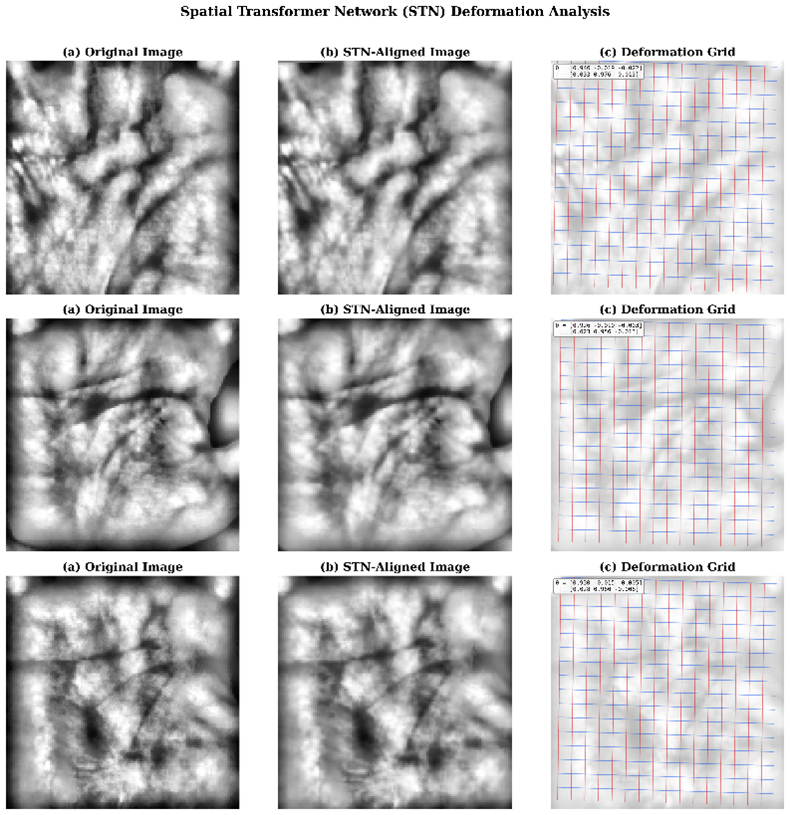
\includegraphics[width=\columnwidth]{fig_stn_analysis.png}}
\caption{Phân tích biến đổi không gian của mô-đun STN trên ba mẫu tĩnh mạch đại diện.}
\label{fig:stn_analysis}
\end{figure}

\begin{figure}[H]
\centerline{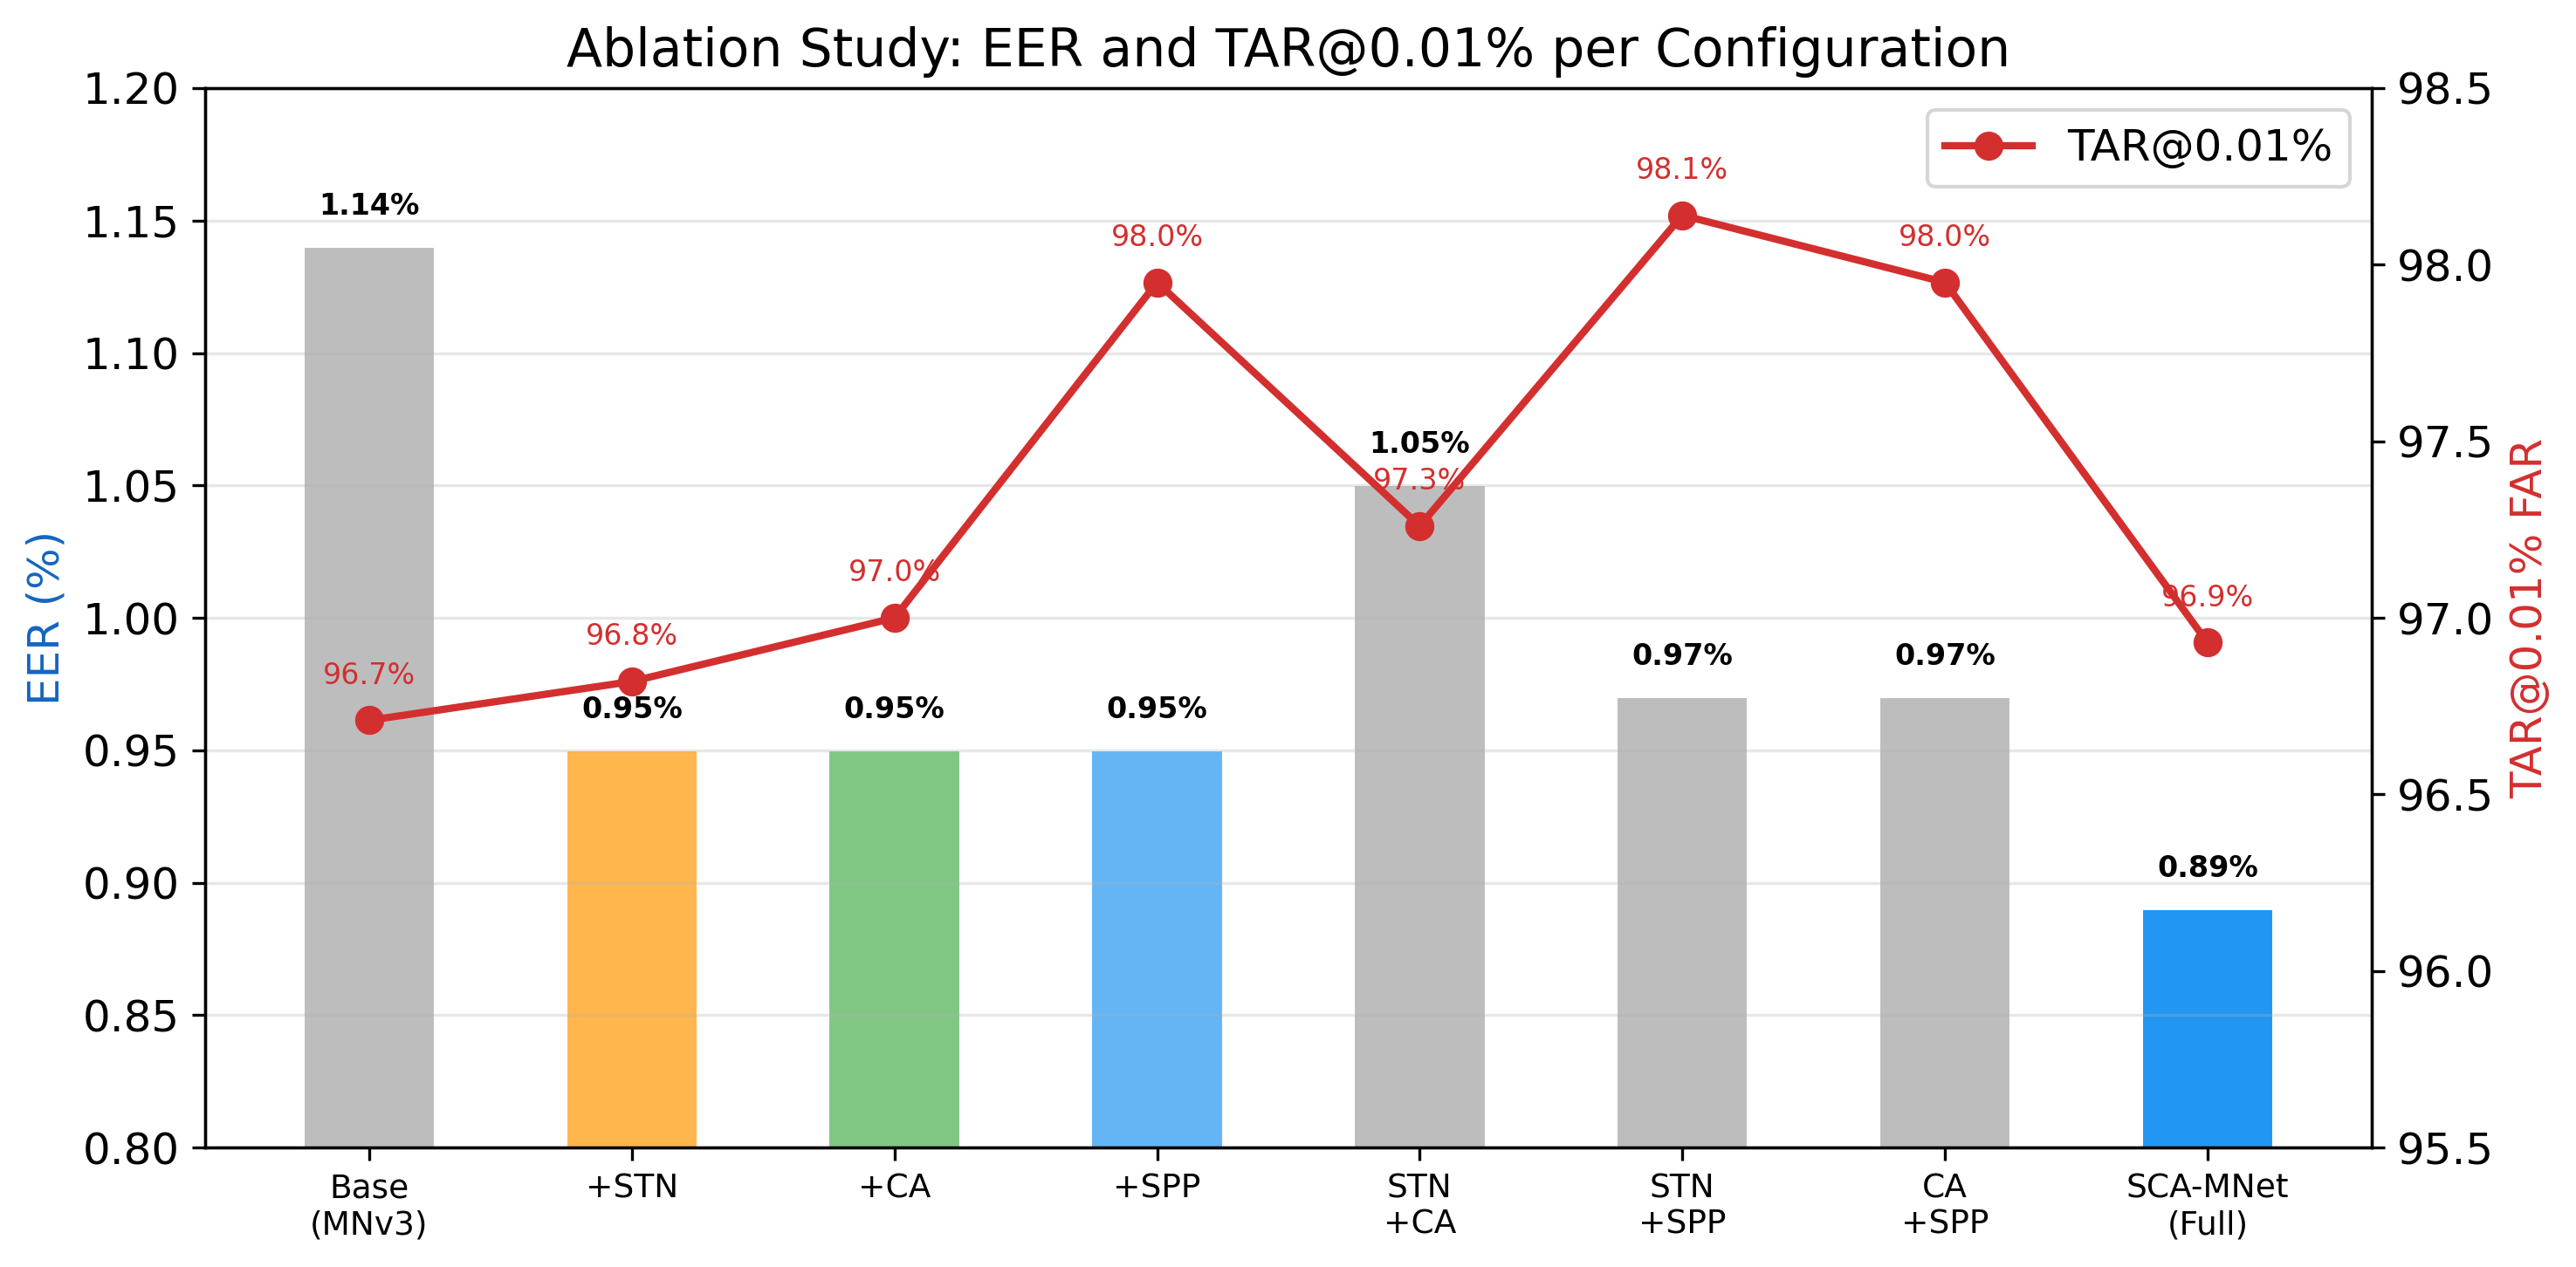
\includegraphics[width=\textwidth]{fig_ablation_bar.png}}
\caption{Biểu đồ cột ablation study trực quan hóa đóng góp của từng module (STN, CA, SPP) vào hiệu năng tổng thể. Trục trái: EER (\%) --- càng thấp càng tốt; Trục phải: TAR@0,01\% --- càng cao càng tốt. Cấu hình 8 (Full SCIB) đạt EER thấp nhất 0,89\% và TAR cao nhất 96,93\%.}
\label{fig:ablation_bar}
\end{figure}

\subsubsection{Ảnh hưởng của tiền xử lý CLAHE}

Để đánh giá đóng góp của bước tăng cường tương phản CLAHE trong pipeline tiền xử lý, chúng tôi tiến hành huấn luyện SCA-MobileNet trên cùng bộ dữ liệu nội bộ (1.549 ID, seed 42, phân chia 70/30 open-set) với hai cấu hình: (1) có CLAHE và (2) không CLAHE. Tất cả các siêu tham số huấn luyện được giữ nguyên.

\begin{table}[H]
\caption{Ảnh hưởng của CLAHE đến hiệu năng SCA-MobileNet trên bộ dữ liệu nội bộ (1.549 ID)}
\begin{center}
\resizebox{\columnwidth}{!}{%
\begin{tabular}{|l|c|c|c|c|c|}
\hline
\textbf{Cấu hình} & \textbf{EER (\%)} & \textbf{TAR@0.01\%} & \textbf{TAR@0.1\%} & \textbf{AUC} & \textbf{D-prime} \\
\hline
Không CLAHE & 1.01 & 96.05\% & 98.10\% & 0.9987 & \textbf{6.52} \\
\textbf{Có CLAHE} & \textbf{0.89} & \textbf{96.93\%} & \textbf{98.49\%} & 0.9983 & 6.49 \\
\hline
\end{tabular}%
}
\label{tab:clahe_ablation}
\end{center}
\end{table}

Bảng~\ref{tab:clahe_ablation} cho thấy CLAHE cải thiện EER từ 1,01\% xuống 0,89\% (giảm tương đối 11,9\%) và nâng TAR@0,01\% từ 96,05\% lên 96,93\%. AUC giảm nhẹ từ 0,9987 xuống 0,9983 và D-prime gần như không thay đổi (6,52 xuống 6,49). Kết quả cho thấy CLAHE chuẩn hóa tương phản cục bộ, thu gọn phần đuôi phân phối genuine (giảm số mẫu cùng danh tính bị gán điểm thấp do biến thiên chiếu sáng), qua đó cải thiện khả năng phân biệt tại các ngưỡng FAR thấp --- chỉ số quan trọng cho ứng dụng sinh trắc thực tế --- trong khi giữ nguyên khả năng tách biệt tổng thể giữa phân phối genuine và impostor.

\subsection{So sánh với các Phương pháp Tiên tiến (SOTA)}

Bảng~\ref{tab:sota} so sánh SCA-MobileNet với các phương pháp sinh trắc chuyên dụng giai đoạn 2021--2024: FGFNet \cite{b5} (FFT + FFC), GSCL \cite{b3} (học tự giám sát + dữ liệu tổng hợp), và RSNet \cite{b4} (Siamese hai nhánh).

\textbf{Trên bộ dữ liệu nội bộ (1.549 ID):}
Trong nhóm backbone tổng quát, ResNet-50 (23,51M) đạt EER 4,33\% --- cho thấy backbone nặng không đảm bảo hiệu năng trên bài toán sinh trắc. EfficientNet-B0 (4,01M) đạt 1,77\%, DeiT-Tiny và Swin-Tiny lần lượt 2,22\% và 2,33\%. Đáng chú ý, MobileNetV3 Base (1,52M) --- phiên bản không có STN, CA, SPP --- đạt EER 1,19\%, xác nhận backbone MobileNetV3 phù hợp cho bài toán tĩnh mạch và module SCIB đóng góp thêm 25\% cải thiện (1,19\% $\rightarrow$ 0,89\%).

Trong nhóm phương pháp chuyên dụng, MPSNet đạt EER 1,09\% với 2,99M tham số nhờ cơ chế gộp đa đường. GSCL đạt EER 2,16\% --- backbone ResNet hạn chế hiệu năng dù có cơ chế tăng cường dữ liệu tổng hợp. FGFNet đạt EER 3,93\% và TAR@0,01\% chỉ 77,80\%, cho thấy đặc trưng tần số Fourier không hiệu quả trên tập nội bộ lớn. RSNet đạt EER 2,82\% --- kiến trúc hai nhánh không đủ sức trên 1.549 lớp. SCA-MobileNet đạt EER 0,89\% và TAR 96,93\% với 3,19M tham số --- tốt nhất trong tất cả 12 phương pháp.

\begin{table}[H]
\caption{So sánh hiệu năng SOTA (State-of-the-Art) trên giao thức Open-Set. $\dagger$: mã nguồn công khai, $\ddagger$: tự cài đặt lại.}
\begin{center}
\renewcommand{\arraystretch}{1.2}
\resizebox{\columnwidth}{!}{%
\begin{tabular}{|l|c|c|c|c|c|}
\hline
\textbf{Phương pháp} & \textbf{Khung Thiết Kế} & \textbf{Params(M)} & \textbf{EER (\%)} & \textbf{TAR @ FAR=$10^{-4}$} & \textbf{AUC} \\
\hline
\multicolumn{6}{|c|}{\textbf{Tập dữ liệu Tĩnh mạch lòng bàn tay nội bộ (Đề xuất, 1.549 Cá nhân)}} \\
\hline
MobileNetV3 (Base)$^\ddagger$ & Lightweight CNN & 1.52 & 1.19 & 95.69\% & 0.9977 \\
MPSNet$^\dagger$ & Multi-path SPP & 2.99 & 1.09 & 96.96\% & 0.9979 \\
EfficientNet-B0$^\ddagger$ & Compound Scaling & 4.01 & 1.77 & 93.03\% & 0.9965 \\
DeiT-Tiny$^\ddagger$ & Vision Transformer & 5.52 & 2.22 & 92.17\% & 0.9959 \\
FGFNet$^\dagger$ \cite{b5} & Fourier Transform & 5.62 & 3.93 & 77.80\% & 0.9904 \\
MobileViT-S$^\ddagger$ & Mobile Transformer & 4.94 & 1.28 & 95.58\% & 0.9977 \\
RSNet$^\ddagger$ \cite{b4} & Siamese Dual-branch & 6.23 & 2.82 & 89.39\% & 0.9936 \\
GSCL$^\dagger$ \cite{b3} & Generative Self-Sup & 11.23 & 2.16 & 89.70\% & 0.9958 \\
ResNet-50$^\ddagger$ & Deep Residual & 23.51 & 4.33 & 62.18\% & 0.9904 \\
Swin-Tiny$^\ddagger$ & Shifted Window & 27.52 & 2.33 & 87.84\% & 0.9962 \\
Modified-DenseNet161$^\dagger$ \cite{b2} & Dense Connection & 28.74 & 1.15 & 97.04\% & 0.9977 \\
\textbf{SCA-MobileNet} & STN+CA+SPP Hybrid & \textbf{3.19} & \textbf{0.89} & \textbf{96.93\%} & \textbf{0.9983} \\
\hline
\end{tabular}%
}
\label{tab:sota}
\end{center}
\end{table}

\subsection{Đánh giá trên bộ dữ liệu mở TONGJI}

Nhằm kiểm chứng khả năng tổng quát hóa, tất cả mô hình được huấn luyện lại từ đầu trên TONGJI với cùng giao thức open-set. Bộ dữ liệu TONGJI cung cấp sẵn ảnh ROI ($128 \times 128$), nên chỉ cần CLAHE và chuẩn hóa kích thước trước khi đưa vào mô hình.

Dù chỉ số TAR@0,01\% trên TONGJI có độ nhạy cảm cao do số lượng mẫu impostor hạn chế, chúng tôi vẫn trình bày chỉ số này đi kèm với TAR@0,1\% để thiết lập bức tranh so sánh nhất quán với thực nghiệm trên tập tự thu thập.

\begin{table}[H]
\caption{So sánh hiệu năng trên bộ dữ liệu TONGJI (giao thức Open-Set, 360 định danh kiểm thử). $\dagger$: mã nguồn công khai, $\ddagger$: tự cài đặt lại. ``---'': đang bổ sung.}
\begin{center}
\resizebox{\columnwidth}{!}{%
\begin{tabular}{l|l|c|c|c|c}
\hline
\textbf{Model} & \textbf{Source} & \textbf{EER (\%)} & \textbf{TAR@0.01\%} & \textbf{TAR@0.1\%} & \textbf{AUC} \\
\hline
MPSNet$^\dagger$ & \cite{b1} & 0.26 & 84.20\% & 99.33\% & 0.9997 \\
Modified-DenseNet161$^\dagger$ & \cite{b2} & 0.39 & 80.87\% & 99.16\% & 0.9998 \\
GSCL$^\dagger$ & \cite{b3} & 1.73 & 58.12\% & 88.01\% & 0.9985 \\
RSNet$^\ddagger$ & \cite{b4} & 1.40 & 75.56\% & 94.02\% & 0.9989 \\
FGFNet$^\dagger$ & \cite{b5} & 5.52 & 55.09\% & 71.78\% & 0.9872 \\
MobileNetV3 (Base)$^\ddagger$ & \cite{b10} & 0.29 & 80.03\% & 99.23\% & 0.9999 \\
EfficientNet-B0$^\ddagger$ & \cite{b20} & 0.57 & 74.61\% & 98.15\% & 0.9996 \\
ResNet50$^\ddagger$ & \cite{b3} & 0.72 & 86.54\% & 97.07\% & 0.9997 \\
Swin-Tiny$^\ddagger$ & --- & 1.13 & 70.01\% & 93.86\% & 0.9990 \\
DeiT-Tiny$^\ddagger$ & --- & 1.93 & 68.50\% & 88.70\% & 0.9979 \\
MobileViT-S$^\ddagger$ & --- & 1.32 & 76.12\% & 93.80\% & 0.9984 \\
\hline
\textbf{SCA-MobileNet} & \textbf{Ours} & \textbf{0.06} & \textbf{90.06\%} & \textbf{99.95\%} & \textbf{0.9999} \\
\hline
\end{tabular}%
}
\label{tab:tongji_results}
\end{center}
\end{table}

Bảng \ref{tab:tongji_results} cho thấy SCA-MobileNet đạt EER 0,06\% trên TONGJI, vượt mô hình xếp thứ hai (MPSNet, EER 0,26\%). Tại FAR = 0,01\%, SCA-MobileNet đạt TAR 90,06\% và TAR@0,1\% đạt 99,95\%. Chỉ số d-prime đạt 8,56 --- cao hơn đáng kể so với các baseline --- phản ánh không gian embedding có độ phân biệt cao.

\begin{table}[H]
\caption{Đánh giá Hiệu năng Chi tiết trên hai bộ dữ liệu thực nghiệm}
\begin{center}
\renewcommand{\arraystretch}{1.2}
\resizebox{\columnwidth}{!}{%
\begin{tabular}{|l|c|c|c|}
\hline
\textbf{Metric} & \textbf{SCA-MobileNet} & \textbf{Runner-up (MPSNet)} & \textbf{Tăng trưởng} \\
\hline
\multicolumn{4}{|c|}{\textbf{Tập dữ liệu Tĩnh mạch lòng bàn tay nội bộ (Đề xuất)}} \\
\hline
EER (\%) & \textbf{0.89} & 1.09 & \textcolor{blue}{$\downarrow$ 18.3\%} \\
TAR @ FAR=$10^{-2}$ & \textbf{99.12\%} & 98.85\% & \textcolor{red}{$\uparrow$ 0.27\%} \\
TAR @ FAR=$10^{-3}$ & \textbf{98.49\%} & 98.06\% & \textcolor{red}{$\uparrow$ 0.43\%} \\
TAR @ FAR=$10^{-4}$ & 96.93\% & \textbf{96.96\%} & $\approx$ 0.00\% \\
AUC & \textbf{0.9983} & 0.9979 & \textcolor{red}{$\uparrow$ 0.0004} \\
d-prime ($d'$) & \textbf{6.49} & 6.24 & \textcolor{red}{$\uparrow$ 0.25} \\
\hline
\multicolumn{4}{|c|}{\textbf{Tập dữ liệu TONGJI (Vân lòng bàn tay)}} \\
\hline
EER (\%) & \textbf{0.06} & 0.26 & \textcolor{blue}{$\downarrow$ 76.9\%} \\
TAR @ FAR=$10^{-2}$ & \textbf{99.99\%} & 99.81\% & \textcolor{red}{$\uparrow$ 0.18\%} \\
TAR @ FAR=$10^{-3}$ & \textbf{99.95\%} & 99.33\% & \textcolor{red}{$\uparrow$ 0.62\%} \\
TAR @ FAR=$10^{-4}$ & \textbf{90.06\%} & 84.20\% & \textcolor{red}{$\uparrow$ 5.86\%} \\
AUC & \textbf{0.9999} & 0.9997 & \textcolor{red}{$\uparrow$ 0.0002} \\
d-prime ($d'$) & \textbf{8.56} & 6.96 & \textcolor{red}{$\uparrow$ 1.60} \\
\hline
\end{tabular}%
}
\label{tab:detailed_metrics}
\end{center}
\end{table}

Kết quả nhất quán trên cả hai bộ dữ liệu --- tĩnh mạch NIR nội bộ và vân lòng bàn tay TONGJI --- cho thấy SCA-MobileNet học được biểu diễn hình học tổng quát cho các cấu trúc đường nét (veins, palmprint) nhờ sự kết hợp STN (căn chỉnh hình học), CA (định vị cấu trúc), và SPP (tổng hợp đa thang đo).

\begin{figure}[H]
\centerline{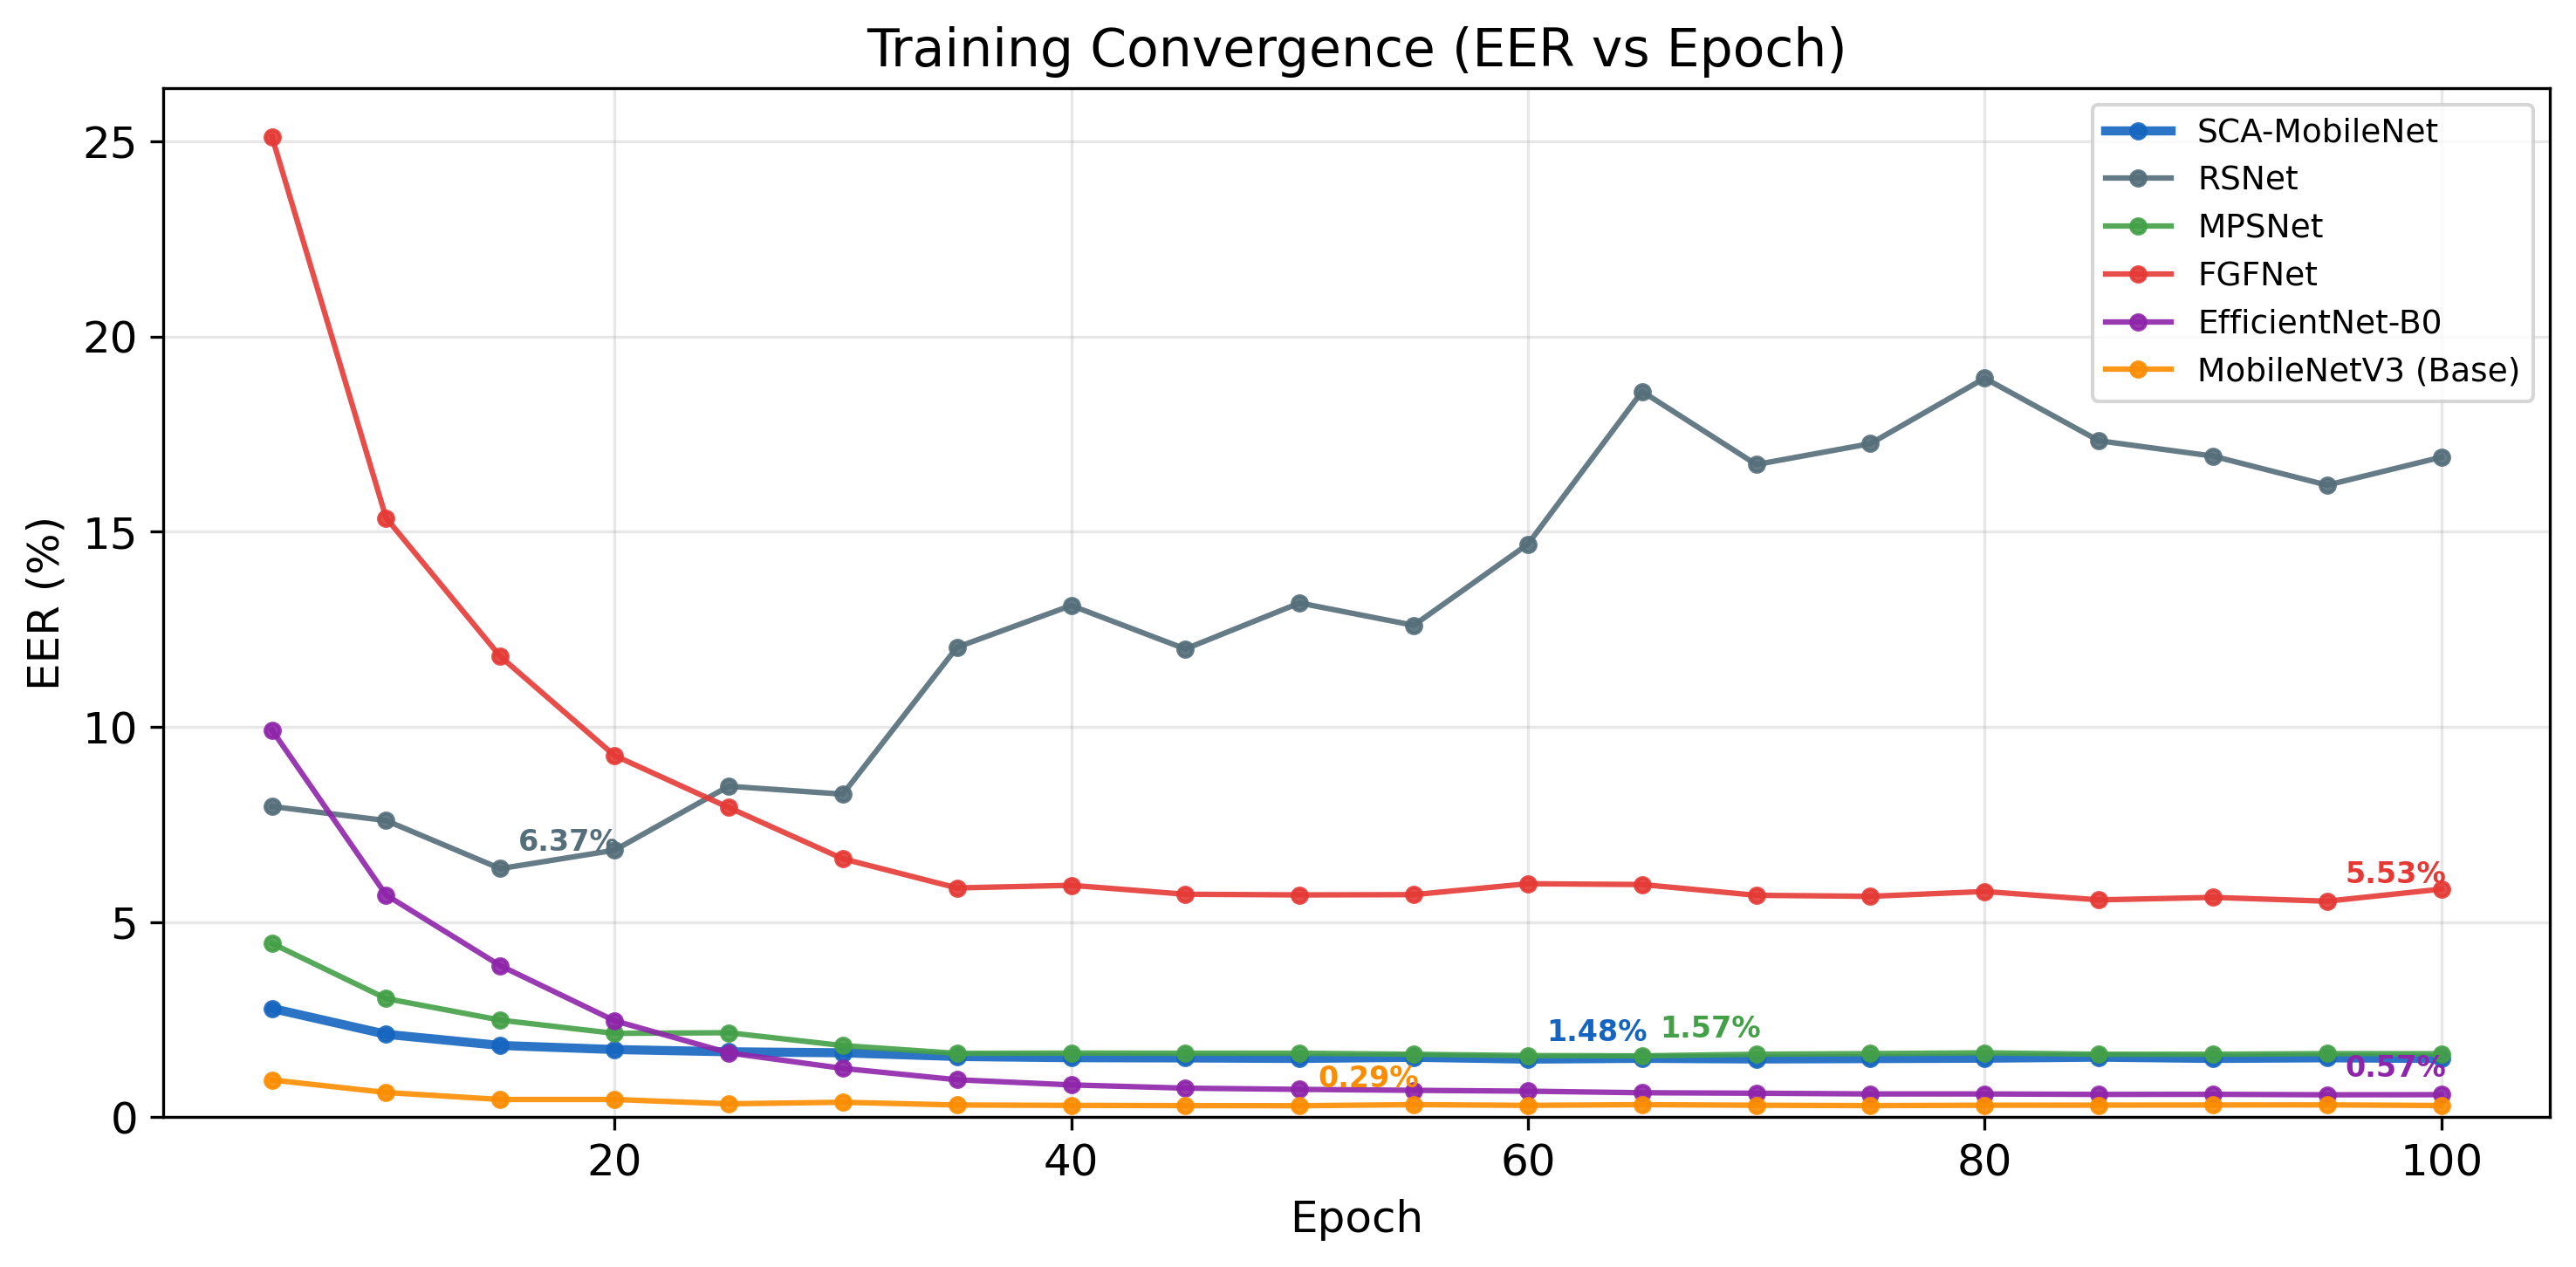
\includegraphics[width=\textwidth]{fig_training_convergence.png}}
\caption{Đường cong hội tụ huấn luyện (EER vs. Epoch) trên các mô hình đại diện. SCA-MobileNet hội tụ nhanh và ổn định, đạt EER thấp nhất từ epoch sớm. Các điểm đánh dấu chỉ ra epoch đạt EER tối ưu cho mỗi mô hình.}
\label{fig:training_convergence}
\end{figure}

\subsection{Đánh giá trên bộ dữ liệu SCUT}

Tất cả 12 mô hình được huấn luyện từ đầu trên SCUT FVP với cùng giao thức open-set. Tương tự TONGJI, ảnh SCUT đã có sẵn ROI, chỉ qua CLAHE và chuẩn hóa Z-score.

\begin{table}[H]
\caption{So sánh hiệu năng trên bộ dữ liệu SCUT (giao thức Open-Set, 330 định danh kiểm thử). $\dagger$: mã nguồn công khai, $\ddagger$: tự cài đặt lại.}
\begin{center}
\resizebox{\textwidth}{!}{%
\begin{tabular}{l|l|c|c|c|c|c}
\hline
\textbf{Model} & \textbf{Source} & \textbf{EER (\%)} & \textbf{TAR@0.01\%} & \textbf{TAR@0.1\%} & \textbf{TAR@1\%} & \textbf{AUC} \\
\hline
\textbf{SCA-MobileNet} & \textbf{Ours} & \textbf{1.48} & \textbf{88.10\%} & \textbf{95.00\%} & \textbf{98.10\%} & \textbf{0.9986} \\
Modified-DenseNet161$^\dagger$ & \cite{b2} & 1.51 & 90.80\% & 95.00\% & 98.10\% & 0.9983 \\
MPSNet$^\dagger$ & \cite{b1} & 1.57 & 88.00\% & 93.20\% & 97.90\% & 0.9978 \\
MobileNetV3 (Base)$^\ddagger$ & \cite{b10} & 2.33 & 85.00\% & 90.10\% & 95.90\% & 0.9968 \\
EfficientNet-B0$^\ddagger$ & \cite{b20} & 3.02 & 63.20\% & 78.90\% & 93.00\% & 0.9959 \\
ResNet50$^\ddagger$ & \cite{b3} & 3.38 & 63.23\% & 81.96\% & 93.00\% & 0.9948 \\
GSCL$^\dagger$ & \cite{b3} & 3.42 & 74.60\% & 80.10\% & 92.20\% & 0.9947 \\
Swin-Tiny$^\ddagger$ & --- & 3.71 & 47.80\% & 70.90\% & 90.00\% & 0.9937 \\
MobileViT-S$^\ddagger$ & --- & 4.94 & 42.80\% & 64.00\% & 85.60\% & 0.9905 \\
DeiT-Tiny$^\ddagger$ & --- & 5.04 & 42.40\% & 61.40\% & 84.30\% & 0.9896 \\
FGFNet$^\dagger$ & \cite{b5} & 5.53 & 49.40\% & 62.30\% & 84.00\% & 0.9873 \\
RSNet$^\ddagger$ & \cite{b4} & 6.37 & 51.30\% & 65.40\% & 83.50\% & 0.9833 \\
\hline
\end{tabular}%
}
\label{tab:scut_results}
\end{center}
\end{table}

Bảng~\ref{tab:scut_results} cho thấy SCA-MobileNet đạt EER 1,48\% trên SCUT, tiếp theo là Modified-DenseNet161 (1,51\%) và MPSNet (1,57\%). Modified-DenseNet161 đạt TAR@0,01\% cao hơn (90,80\% so với 88,10\%) nhờ backbone DenseNet ($\sim$28M params), nhưng SCA-MobileNet dẫn đầu về EER với chỉ 3,19M tham số. RSNet đạt EER 6,37\% trên SCUT --- sụt giảm đáng kể so với hiệu năng trên TONGJI --- cho thấy thiết kế dual-branch không tổng quát tốt trên dữ liệu palmprint visible. Các transformer backbone (Swin-Tiny, DeiT-Tiny) đạt EER 3,71--5,04\%, phản ánh khó khăn khi huấn luyện transformer trên bộ dữ liệu kích thước trung bình.

\textbf{Phân tích tính ổn định (Multi-seed):} Để đánh giá tính tái lập, SCA-MobileNet được huấn luyện 5 lần trên SCUT với các seed ngẫu nhiên khác nhau (42, 0, 1, 7, 99). Bảng~\ref{tab:multi_seed} cho thấy EER trung bình đạt $1{,}46\% \pm 0{,}04\%$ (khoảng tin cậy 95\%: $[1{,}42\%,~1{,}50\%]$), xác nhận tính ổn định cao của kiến trúc đề xuất.

\begin{table}[H]
\caption{Phân tích tính ổn định SCA-MobileNet trên SCUT qua 5 seed ngẫu nhiên.}
\begin{center}
\begin{tabular}{c|c}
\hline
\textbf{Seed} & \textbf{EER (\%)} \\
\hline
42 & 1,46 \\
0 & 1,48 \\
1 & 1,48 \\
7 & 1,49 \\
99 & 1,39 \\
\hline
\textbf{Trung bình $\pm$ Std} & $\mathbf{1{,}46 \pm 0{,}04}$ \\
\textbf{KTC 95\%} & $[1{,}42,~1{,}50]$ \\
\hline
\end{tabular}
\label{tab:multi_seed}
\end{center}
\end{table}

\subsection{Đánh giá trên bộ dữ liệu VERA}

Bộ dữ liệu VERA đặt ra thách thức: phương thức NIR tương tự bộ nội bộ nhưng từ thiết bị khác, và chỉ 220 định danh với 5 mẫu/ID --- quy mô nhỏ nhất. Tất cả mô hình được huấn luyện từ đầu với giao thức open-set tương tự.

\begin{table}[H]
\caption{So sánh hiệu năng trên bộ dữ liệu VERA Palmvein (giao thức Open-Set, 66 định danh kiểm thử). $\dagger$: mã nguồn công khai, $\ddagger$: tự cài đặt lại.}
\begin{center}
\resizebox{\textwidth}{!}{%
\begin{tabular}{l|l|c|c|c|c|c}
\hline
\textbf{Model} & \textbf{Source} & \textbf{EER (\%)} & \textbf{TAR@0.01\%} & \textbf{TAR@0.1\%} & \textbf{TAR@1\%} & \textbf{AUC} \\
\hline
\textbf{SCA-MobileNet} & \textbf{Ours} & \textbf{2.76} & \textbf{86.20\%} & \textbf{90.90\%} & \textbf{95.60\%} & \textbf{0.9950} \\
MobileNetV3 (Base)$^\ddagger$ & \cite{b10} & 3.62 & 76.50\% & 85.50\% & 93.00\% & 0.9935 \\
MPSNet$^\dagger$ & \cite{b1} & 4.87 & 68.00\% & 79.90\% & 90.40\% & 0.9864 \\
Swin-Tiny$^\ddagger$ & --- & 5.69 & 66.80\% & 70.80\% & 83.80\% & 0.9843 \\
DeiT-Tiny$^\ddagger$ & --- & 6.99 & 64.60\% & 70.90\% & 83.10\% & 0.9794 \\
Modified-DenseNet161$^\dagger$ & \cite{b2} & 7.14 & 62.70\% & 71.10\% & 82.80\% & 0.9772 \\
GSCL$^\dagger$ & \cite{b3} & 7.17 & 62.90\% & 65.80\% & 78.70\% & 0.9719 \\
EfficientNet-B0$^\ddagger$ & \cite{b20} & 7.21 & 63.70\% & 67.80\% & 80.70\% & 0.9796 \\
RSNet$^\ddagger$ & \cite{b4} & 8.50 & 61.00\% & 63.90\% & 77.80\% & 0.9664 \\
MobileViT-S$^\ddagger$ & --- & 8.79 & 46.90\% & 53.60\% & 73.30\% & 0.9709 \\
ResNet50$^\ddagger$ & \cite{b3} & 8.89 & 40.80\% & 54.40\% & 74.20\% & 0.9652 \\
FGFNet$^\dagger$ & \cite{b5} & 9.68 & 41.20\% & 48.70\% & 67.60\% & 0.9609 \\
\hline
\end{tabular}%
}
\label{tab:vera_results}
\end{center}
\end{table}

Bảng~\ref{tab:vera_results} cho thấy SCA-MobileNet đạt EER 2,76\% trên VERA, tiếp theo là MobileNetV3 Base (3,62\%) và MPSNet (4,87\%). EER tổng thể cao hơn các bộ dữ liệu khác do số lượng mẫu huấn luyện hạn chế (154 IDs $\times$ 5 mẫu = 770 ảnh).

Modified-DenseNet161 --- đạt EER 1,51\% trên SCUT --- tăng lên 7,14\% trên VERA, cho thấy backbone DenseNet không tổng quát tốt sang phương thức NIR. SCA-MobileNet duy trì hiệu năng ổn định hơn nhờ CA và SPP hoạt động hiệu quả trên cả hai phương thức thu nhận.

Để đánh giá khả năng tổng quát hóa liên miền (\textit{cross-domain}), mô hình huấn luyện trên bộ dữ liệu NIR nội bộ (1.084 định danh) được kiểm thử trực tiếp trên toàn bộ TONGJI (1.200 định danh, 12.000 ảnh) mà không fine-tuning. Hai bộ dữ liệu khác biệt về phương thức (NIR vs. visible), đặc trưng sinh trắc (tĩnh mạch vs. vân lòng bàn tay), và phân bố ảnh. Bảng~\ref{tab:cross_domain} trình bày kết quả cho 6 kiến trúc sinh trắc chuyên dụng.

\begin{table}[H]
\caption{Đánh giá tổng quát hóa liên miền (cross-domain): huấn luyện trên bộ dữ liệu tĩnh mạch tự thu thập, kiểm thử trên toàn bộ TONGJI (1.200 định danh).}
\begin{center}
\resizebox{\columnwidth}{!}{%
\begin{tabular}{l|l|c|c|c|c}
\hline
\textbf{Model} & \textbf{Source} & \textbf{EER (\%)} & \textbf{TAR@0.01\%} & \textbf{TAR@0.1\%} & \textbf{AUC} \\
\hline
MPSNet & \cite{b1} & 4.34 & 62.36\% & 80.10\% & 0.9901 \\
Modified-DenseNet161 & \cite{b2} & 3.74 & 66.59\% & 88.67\% & 0.9926 \\
GSCL & \cite{b3} & 4.48 & 64.08\% & 79.47\% & 0.9896 \\
RSNet & \cite{b4} & 11.99 & 13.55\% & 26.96\% & 0.9504 \\
FGFNet & \cite{b5} & 17.46 & 29.90\% & 44.99\% & 0.8876 \\
\hline
\textbf{SCA-MobileNet} & \textbf{Ours} & \textbf{1.50} & \textbf{71.84\%} & \textbf{94.46\%} & \textbf{0.9981} \\
\hline
\end{tabular}%
}
\label{tab:cross_domain}
\end{center}
\end{table}

Bảng \ref{tab:cross_domain} cho thấy SCA-MobileNet đạt EER 1,50\% trong kịch bản liên miền --- thấp hơn 2,5 lần so với mô hình thứ hai (Modified-DenseNet161, EER 3,74\%). TAR@0,1\% đạt 94,46\%.

Các mô hình so sánh suy giảm đáng kể do học đặc trưng quá đặc thù miền huấn luyện. FGFNet phụ thuộc vào đặc tính tần số của ảnh NIR nên suy giảm mạnh nhất (EER 17,46\%). RSNet cũng giảm đáng kể (EER 11,99\%). SCA-MobileNet duy trì hiệu năng cao nhờ: (1) STN chuẩn hóa hình học bất kể phương thức thu nhận; (2) CA định vị cấu trúc theo tọa độ không gian; và (3) SPP tổng hợp đa thang đo.

\subsection{Đánh giá Tổng quát hóa Liên miền giữa VERA và SCUT}

Thí nghiệm cross-domain bổ sung giữa VERA (NIR, 220 ID) và SCUT (visible, 1.100 ID). Hai bộ dữ liệu khác biệt về phương thức, quy mô, và đặc trưng sinh trắc. Mô hình được huấn luyện trên toàn bộ một bộ dữ liệu và kiểm thử trên bộ còn lại mà không fine-tuning.

\begin{table}[H]
\caption{Đánh giá cross-domain: VERA $\rightarrow$ SCUT (huấn luyện trên VERA, kiểm thử trên toàn bộ SCUT).}
\begin{center}
\resizebox{\columnwidth}{!}{%
\begin{tabular}{l|c|c|c|c}
\hline
\textbf{Model} & \textbf{EER (\%)} & \textbf{TAR@0.01\%} & \textbf{TAR@0.1\%} & \textbf{AUC} \\
\hline
\textbf{SCA-MobileNet} & \textbf{10.13} & \textbf{47.53\%} & \textbf{56.94\%} & \textbf{0.9615} \\
MobileNetV3 (Base) & 12.67 & 25.16\% & 41.41\% & 0.9445 \\
DeiT-Tiny & 13.99 & 8.82\% & 23.44\% & 0.9345 \\
Swin-Tiny & 14.38 & 11.48\% & 29.33\% & 0.9323 \\
EfficientNet-B0 & 15.94 & 16.88\% & 27.07\% & 0.9194 \\
MobileViT-S & 16.92 & 9.88\% & 20.63\% & 0.9097 \\
MPSNet & 21.13 & 18.09\% & 28.17\% & 0.8677 \\
GSCL & 22.46 & 7.81\% & 16.78\% & 0.8592 \\
ResNet50 & 22.69 & 8.09\% & 17.58\% & 0.8576 \\
FGFNet & 23.80 & 4.54\% & 11.85\% & 0.8446 \\
Modified-DenseNet161 & 26.90 & 9.37\% & 16.45\% & 0.8120 \\
\hline
\end{tabular}%
}
\label{tab:cross_domain_vera_scut}
\end{center}
\end{table}

\begin{table}[H]
\caption{Đánh giá cross-domain: SCUT $\rightarrow$ VERA (huấn luyện trên SCUT, kiểm thử trên toàn bộ VERA).}
\begin{center}
\resizebox{\columnwidth}{!}{%
\begin{tabular}{l|c|c|c|c}
\hline
\textbf{Model} & \textbf{EER (\%)} & \textbf{TAR@0.01\%} & \textbf{TAR@0.1\%} & \textbf{AUC} \\
\hline
\textbf{SCA-MobileNet} & \textbf{5.61} & \textbf{78.07\%} & \textbf{82.28\%} & \textbf{0.9814} \\
MobileNetV3 (Base) & 8.44 & 62.78\% & 71.47\% & 0.9685 \\
MPSNet & 8.74 & 52.38\% & 66.43\% & 0.9683 \\
EfficientNet-B0 & 9.85 & 57.27\% & 63.91\% & 0.9603 \\
GSCL & 10.62 & 37.13\% & 55.37\% & 0.9563 \\
ResNet50 & 11.43 & 43.75\% & 52.59\% & 0.9507 \\
MobileViT-S & 11.63 & 40.09\% & 52.75\% & 0.9470 \\
Swin-Tiny & 13.05 & 49.52\% & 57.58\% & 0.9395 \\
DeiT-Tiny & 13.51 & 41.11\% & 48.13\% & 0.9351 \\
FGFNet & 16.17 & 18.75\% & 30.23\% & 0.9226 \\
Modified-DenseNet161 & 21.08 & 33.26\% & 38.43\% & 0.8747 \\
RSNet & 26.11 & 10.32\% & 17.69\% & 0.8167 \\
\hline
\end{tabular}%
}
\label{tab:cross_domain_scut_vera}
\end{center}
\end{table}

Bảng~\ref{tab:cross_domain_vera_scut} và~\ref{tab:cross_domain_scut_vera} trình bày kết quả theo cả hai chiều.

Chiều VERA$\rightarrow$SCUT: SCA-MobileNet đạt EER 10,13\%, thấp hơn 2,5 điểm so với MobileNetV3 Base (12,67\%). Modified-DenseNet161 cho EER 26,90\% --- mô hình nặng nhất nhưng không tổng quát tốt trong chuyển miền.

Chiều SCUT$\rightarrow$VERA: SCA-MobileNet đạt EER 5,61\% và TAR@0,01\% 78,07\%. Hiệu năng tốt hơn do SCUT cung cấp nhiều dữ liệu huấn luyện hơn (770 ID so với 220 ID của VERA).

Kết quả cross-domain VERA$\leftrightarrow$SCUT bổ sung cho thí nghiệm NIR$\rightarrow$TONGJI, cho thấy kiến trúc STN-SCIB hoạt động nhất quán trên nhiều cặp miền khác biệt.

\begin{figure}[H]
\centerline{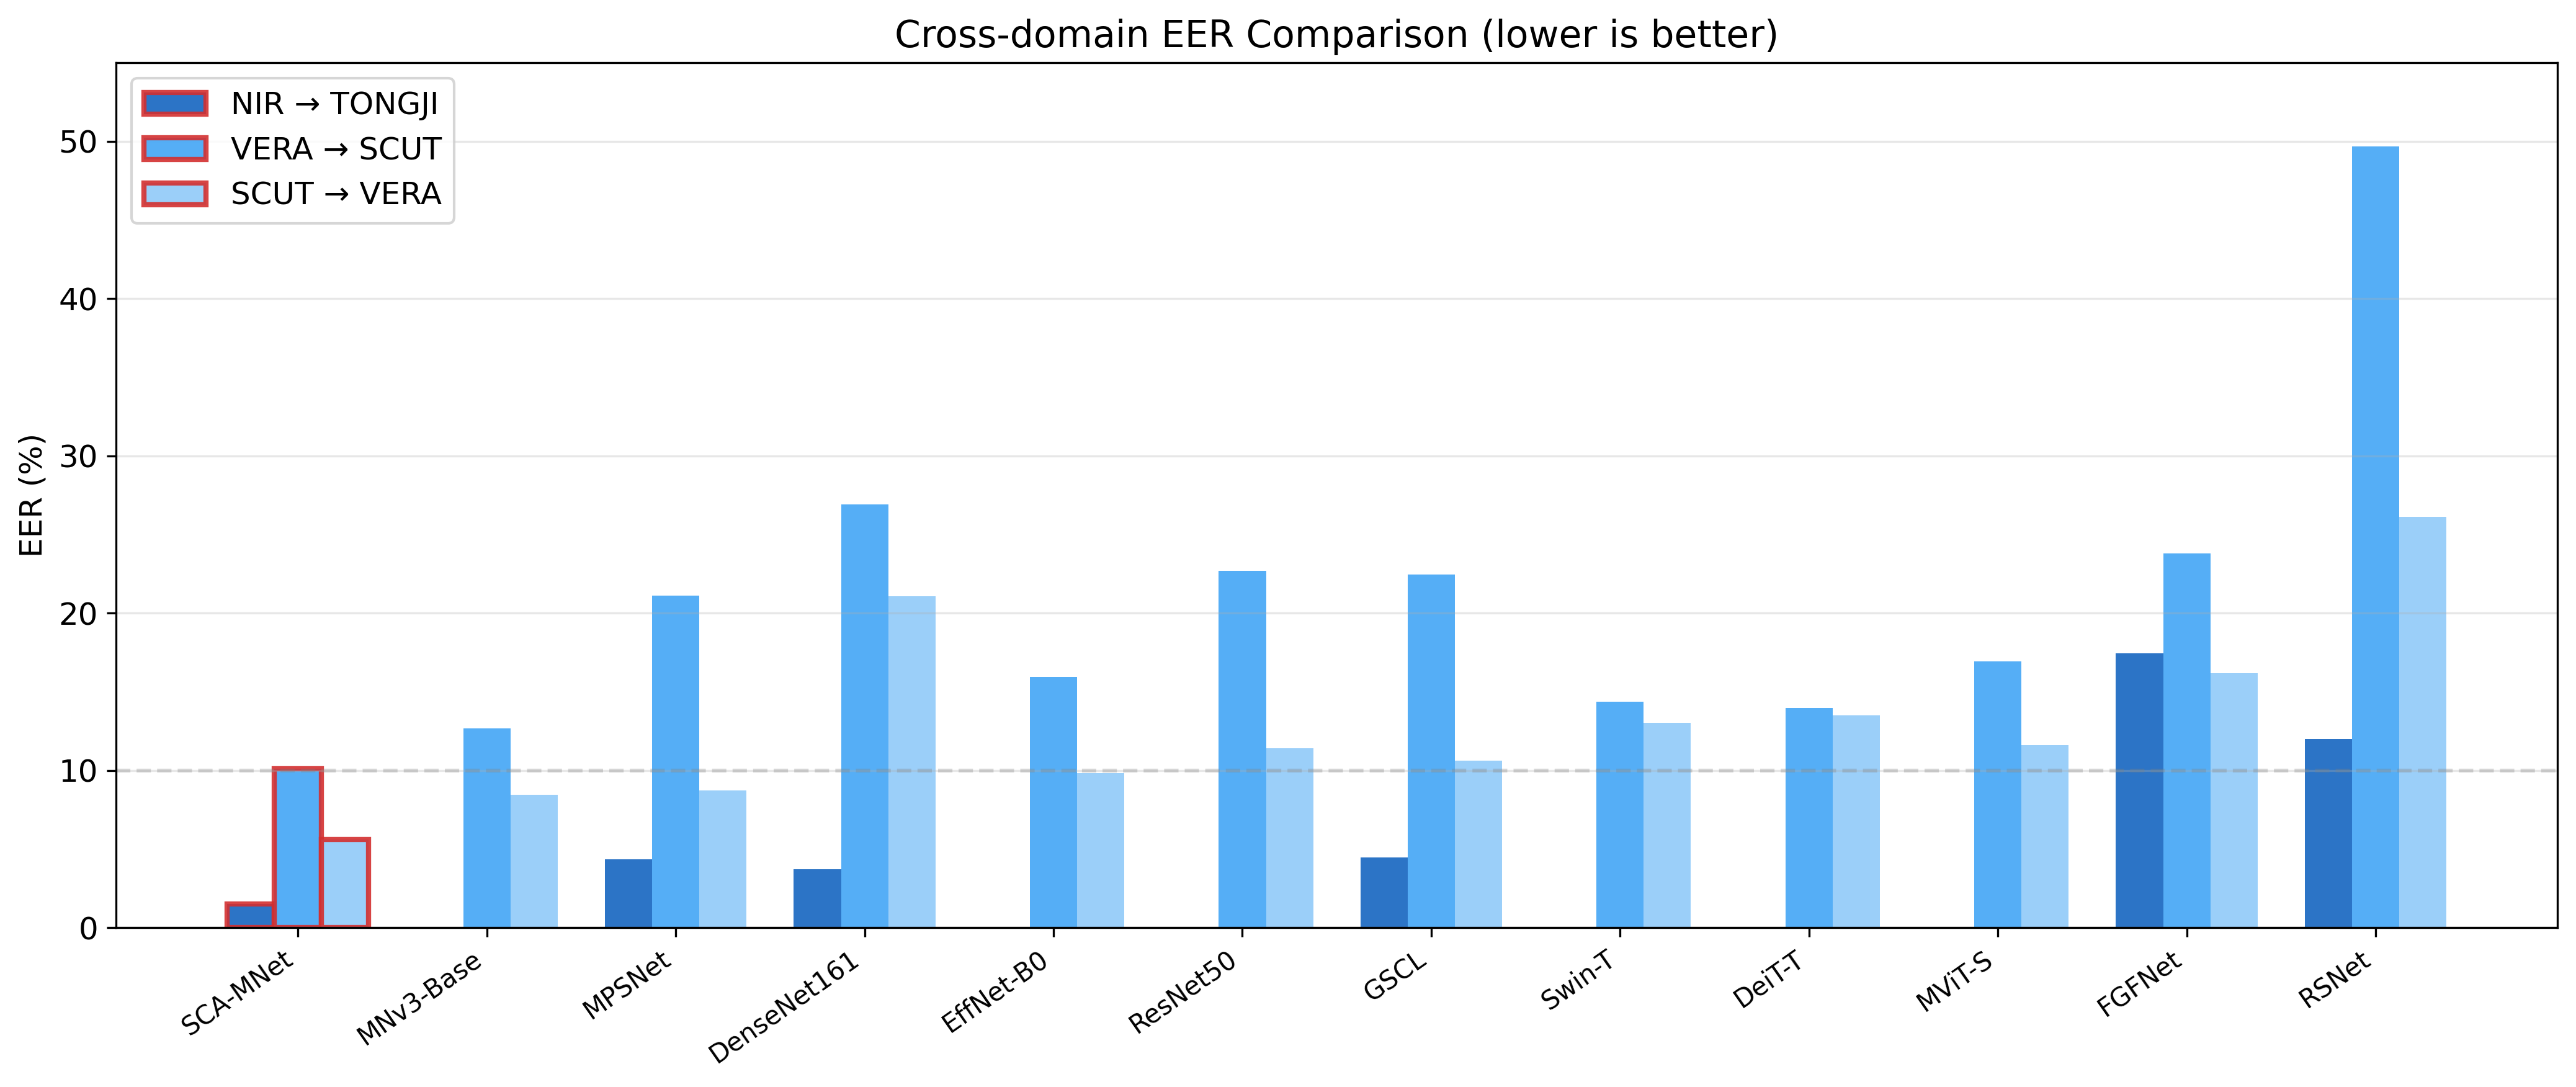
\includegraphics[width=\textwidth]{fig_cross_domain_bar.png}}
\caption{So sánh hiệu năng cross-domain (EER \%) của 12 mô hình trên ba kịch bản chuyển miền: NIR$\rightarrow$TONGJI, VERA$\rightarrow$SCUT, và SCUT$\rightarrow$VERA. SCA-MobileNet (cột xanh đậm) đạt EER thấp nhất nhất quán trên mọi kịch bản. Đường ngang đứt nét chỉ EER trung bình.}
\label{fig:cross_domain_bar}
\end{figure}

\begin{figure}[H]
\centerline{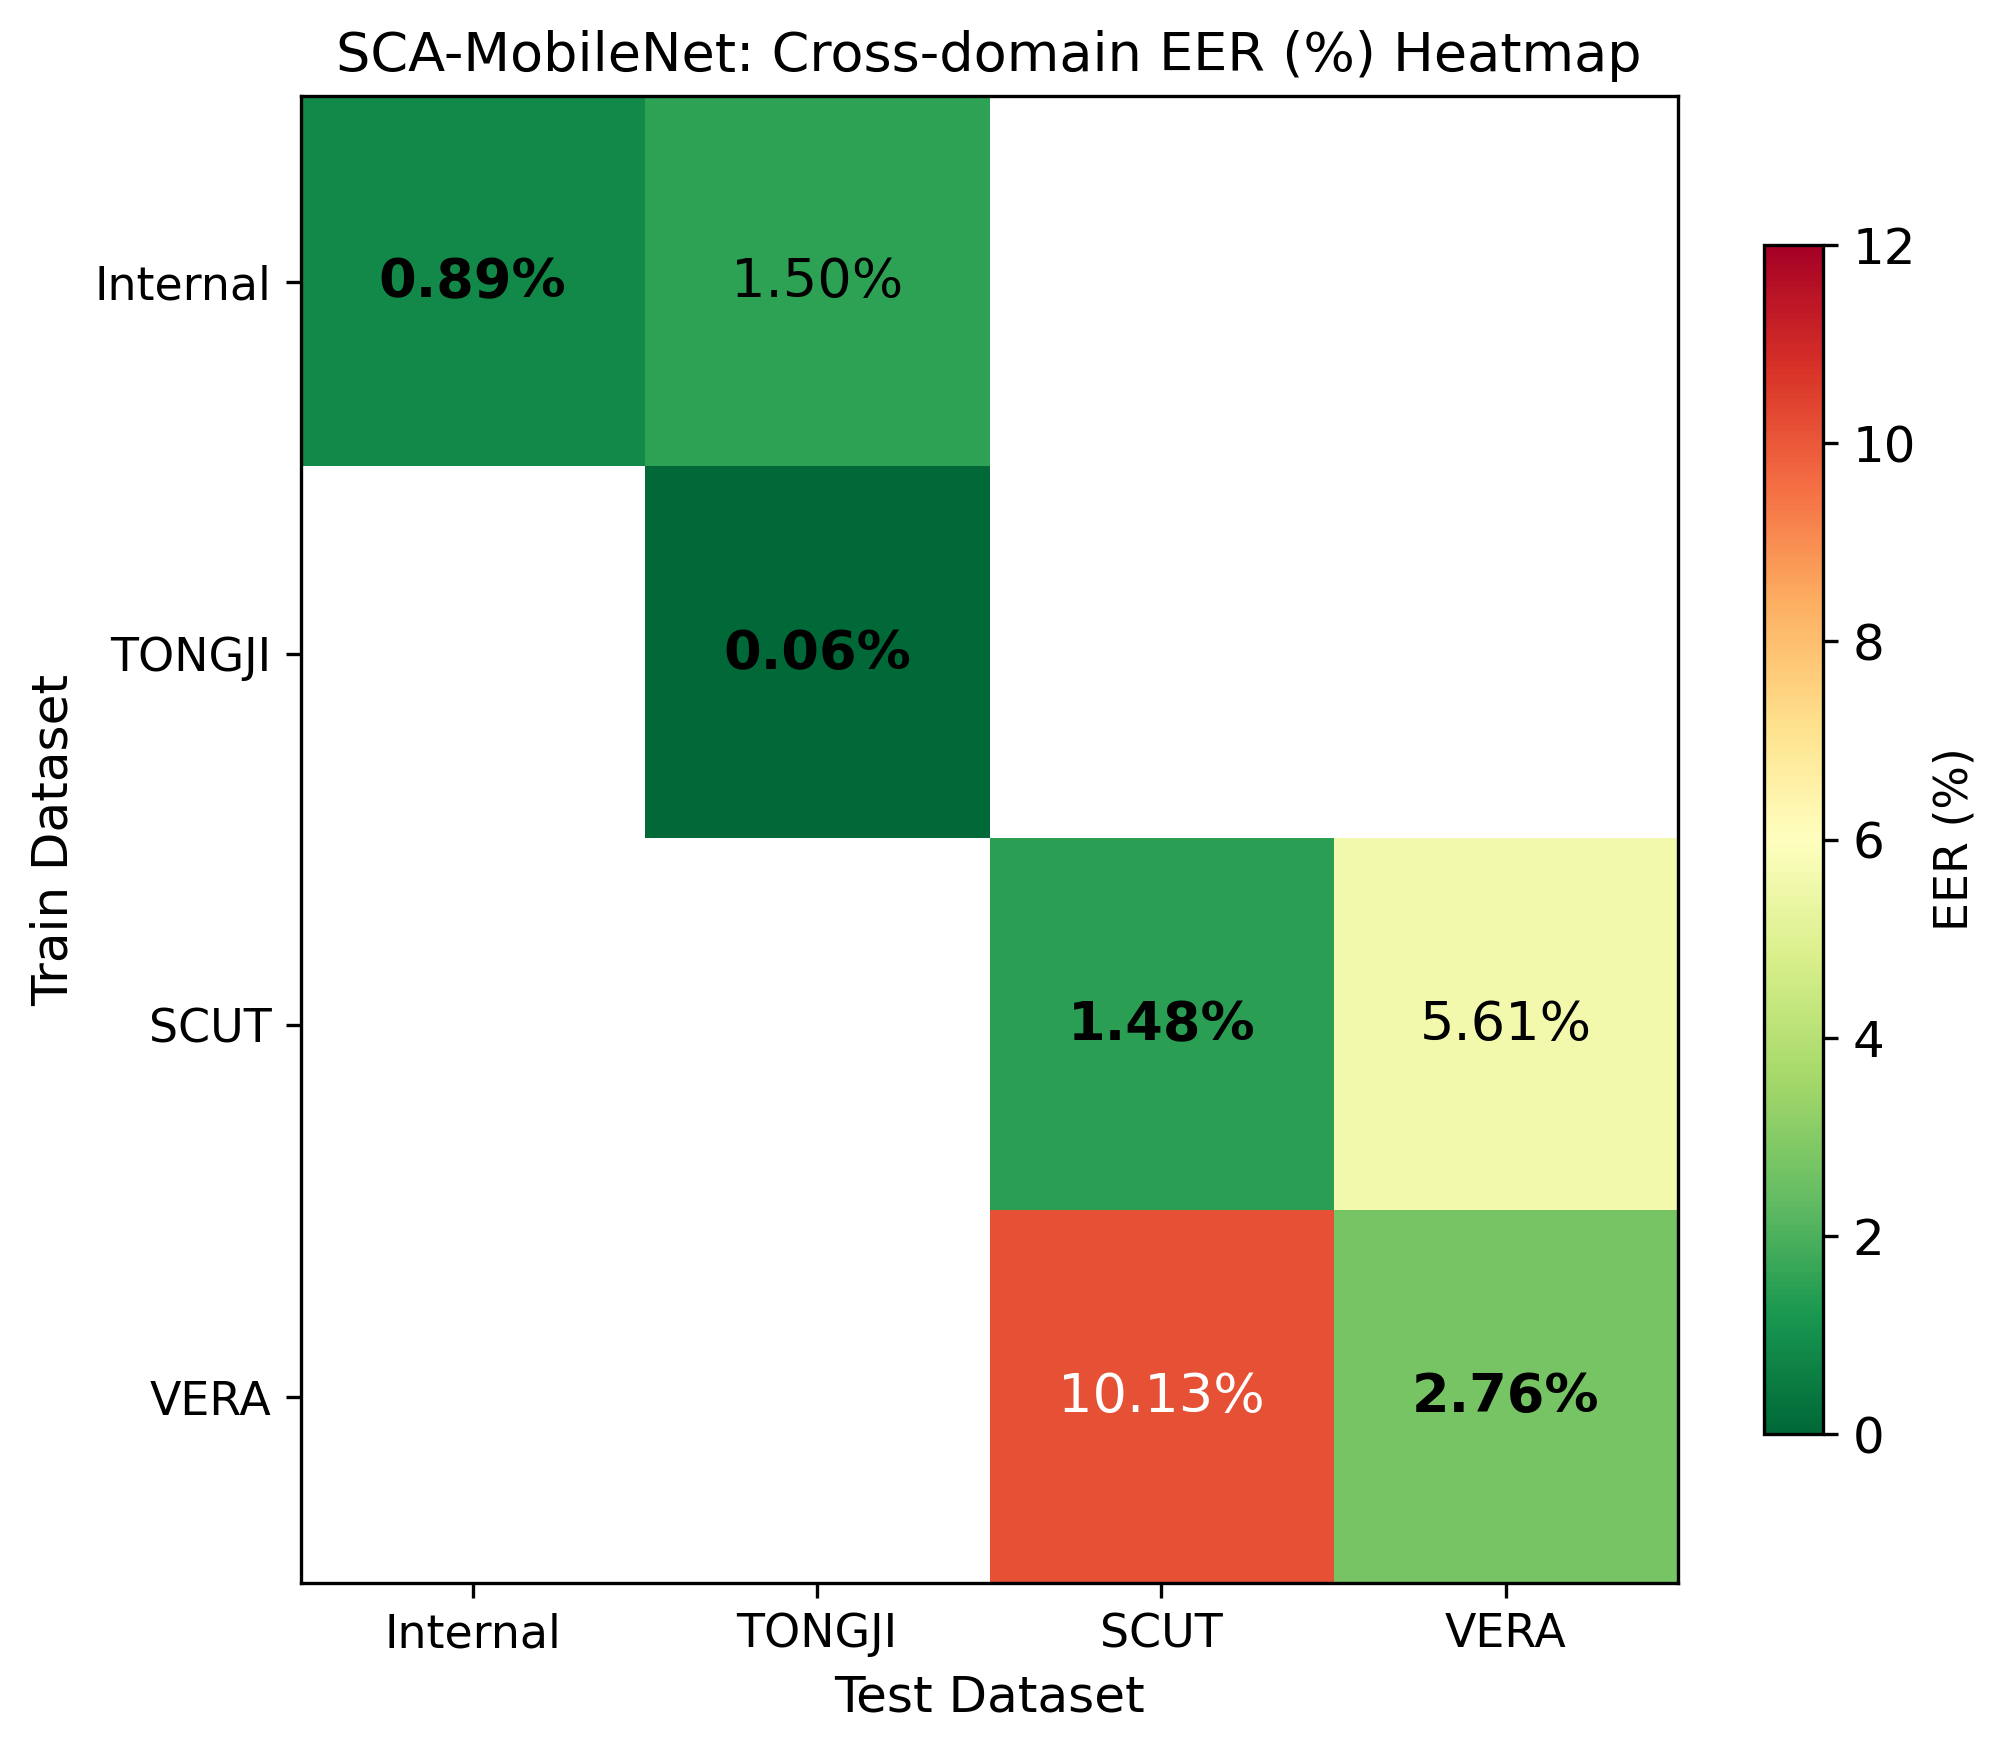
\includegraphics[width=0.7\textwidth]{fig_cross_domain_heatmap.png}}
\caption{Ma trận nhiệt (heatmap) EER cross-domain của SCA-MobileNet. Mỗi ô $(i,j)$ thể hiện EER (\%) khi huấn luyện trên bộ dữ liệu $i$ và kiểm thử trên bộ dữ liệu $j$. Đường chéo chính (in-domain) đạt EER rất thấp; hiệu năng cross-domain suy giảm nhưng vẫn ở mức cạnh tranh.}
\label{fig:cross_domain_heatmap}
\end{figure}

\subsection{Phân tích Đường cong Hiệu năng}

\begin{figure}[H]
\centerline{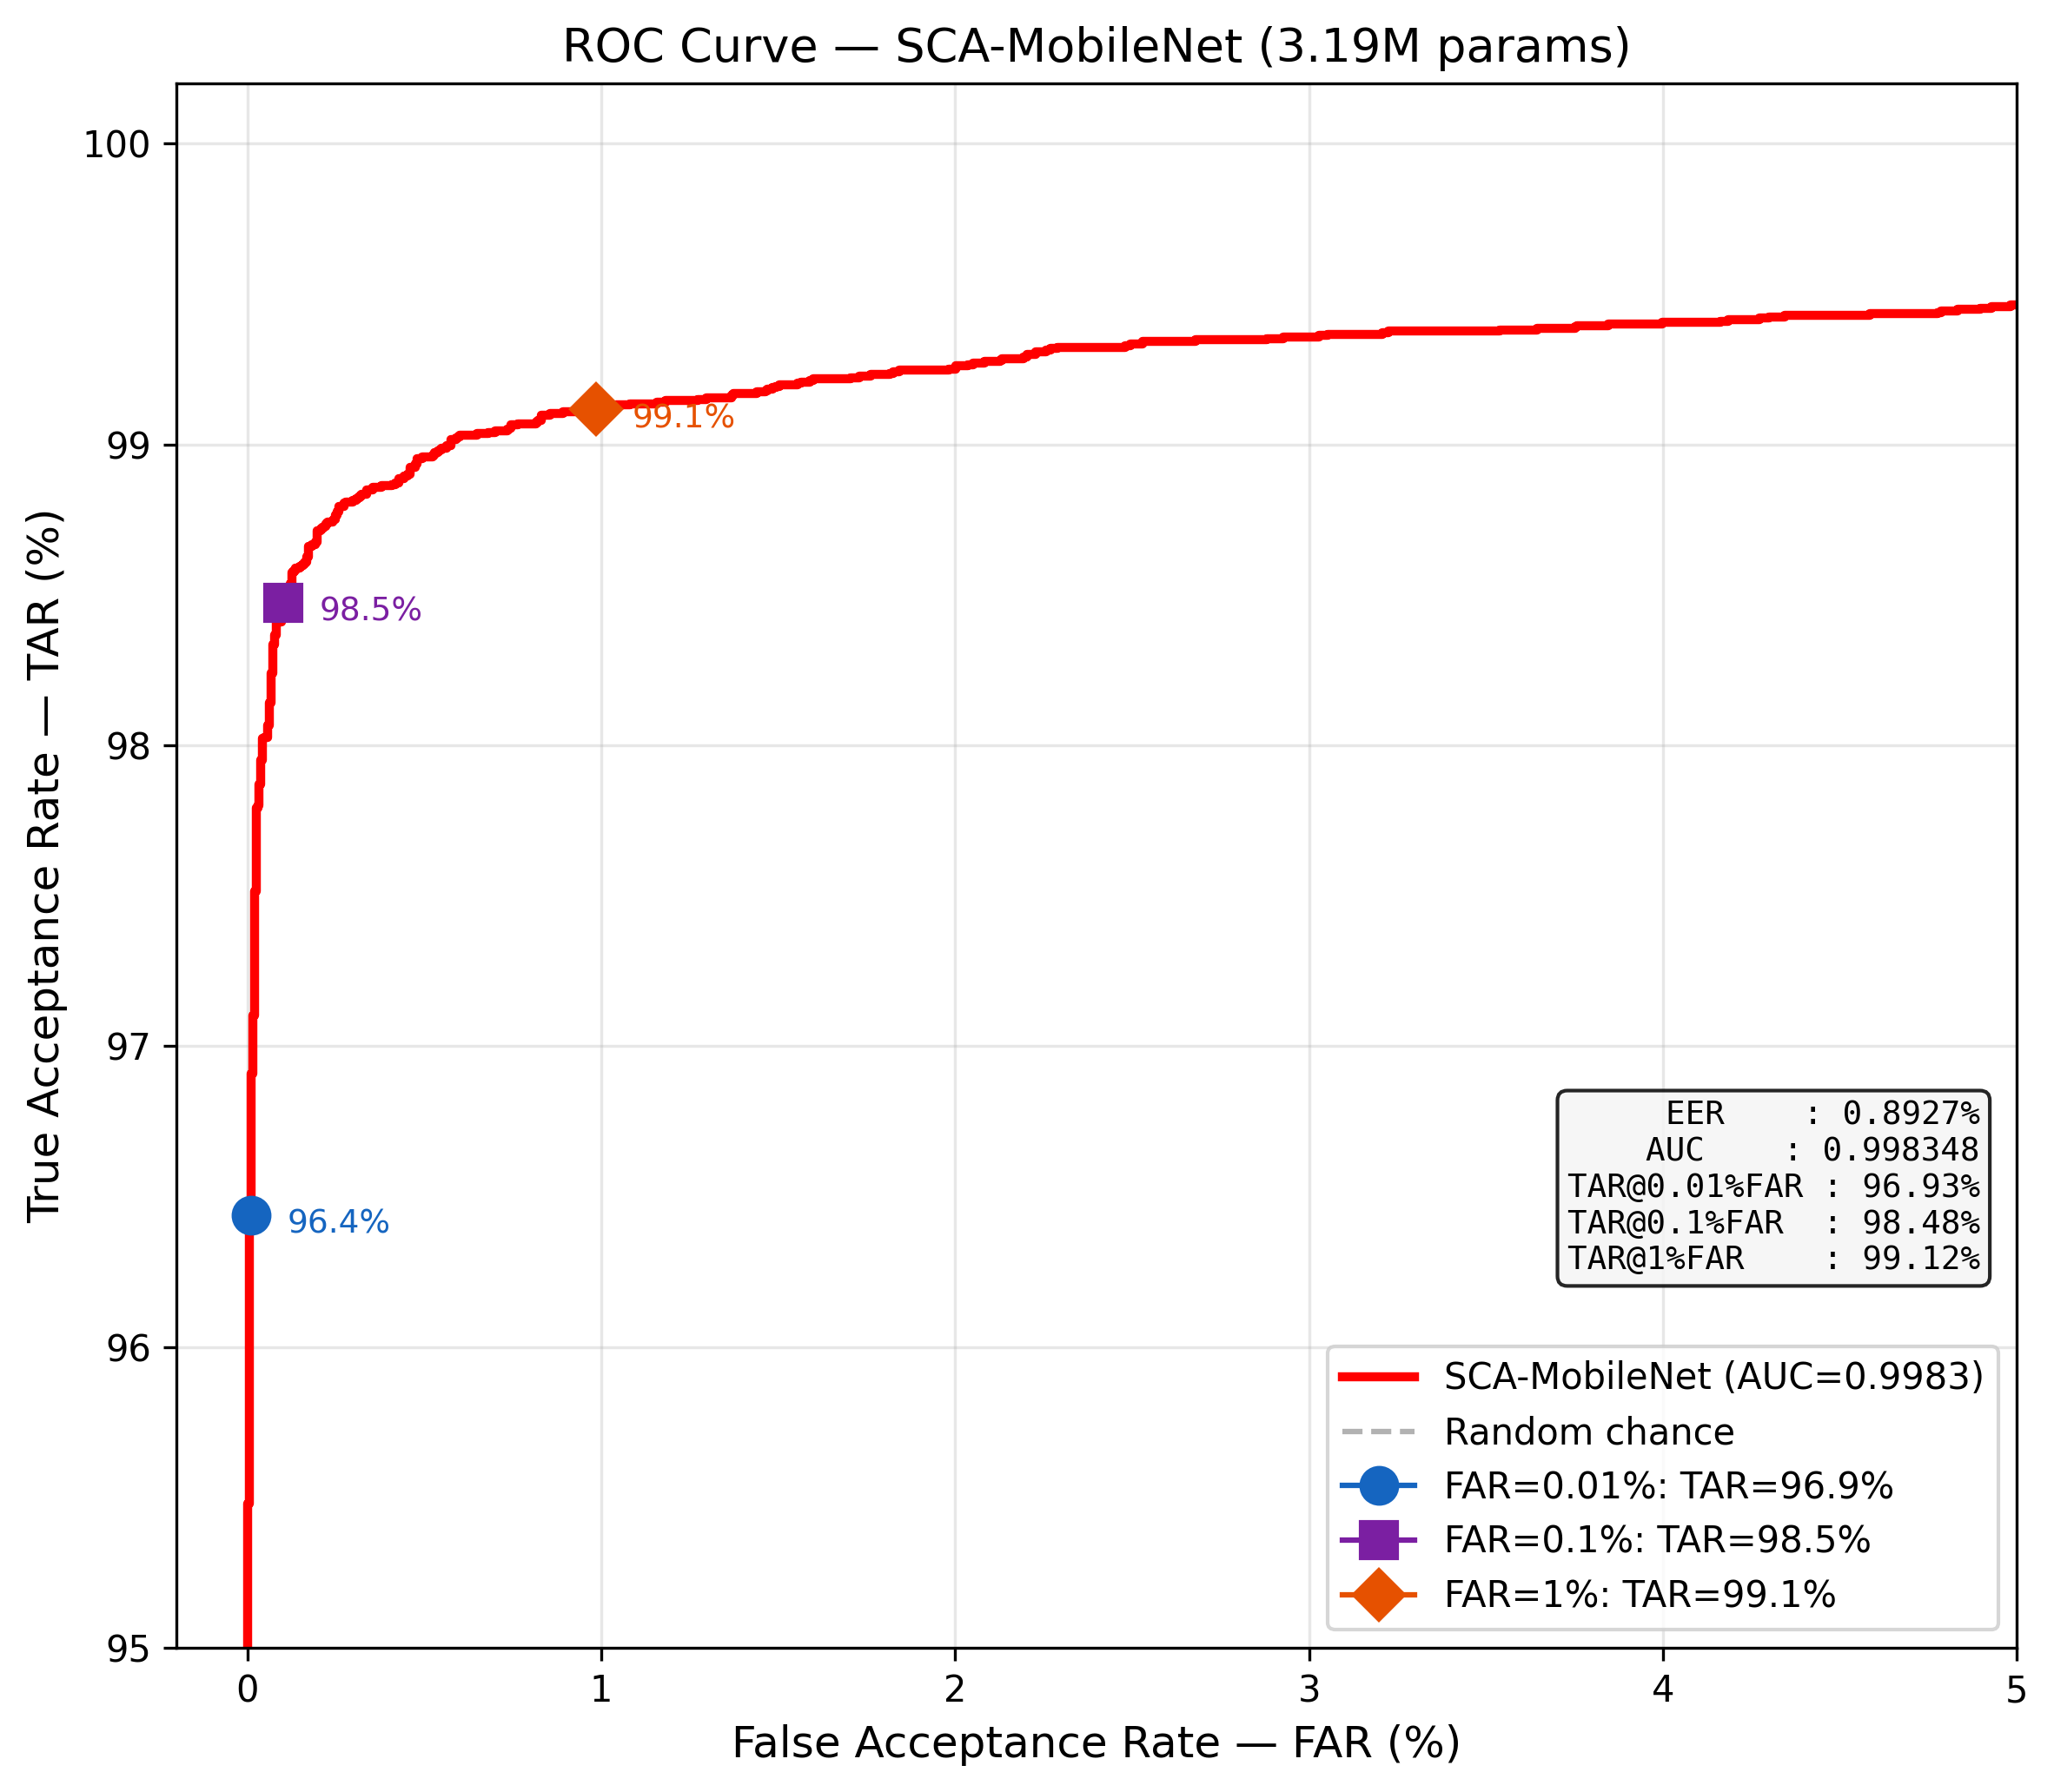
\includegraphics[width=\columnwidth]{fig_roc.png}}
\caption{Đường cong ROC dưới giao thức xác thực open-set (FAR theo thang logarit).}
\label{fig:roc}
\end{figure}

\begin{figure}[H]
\centerline{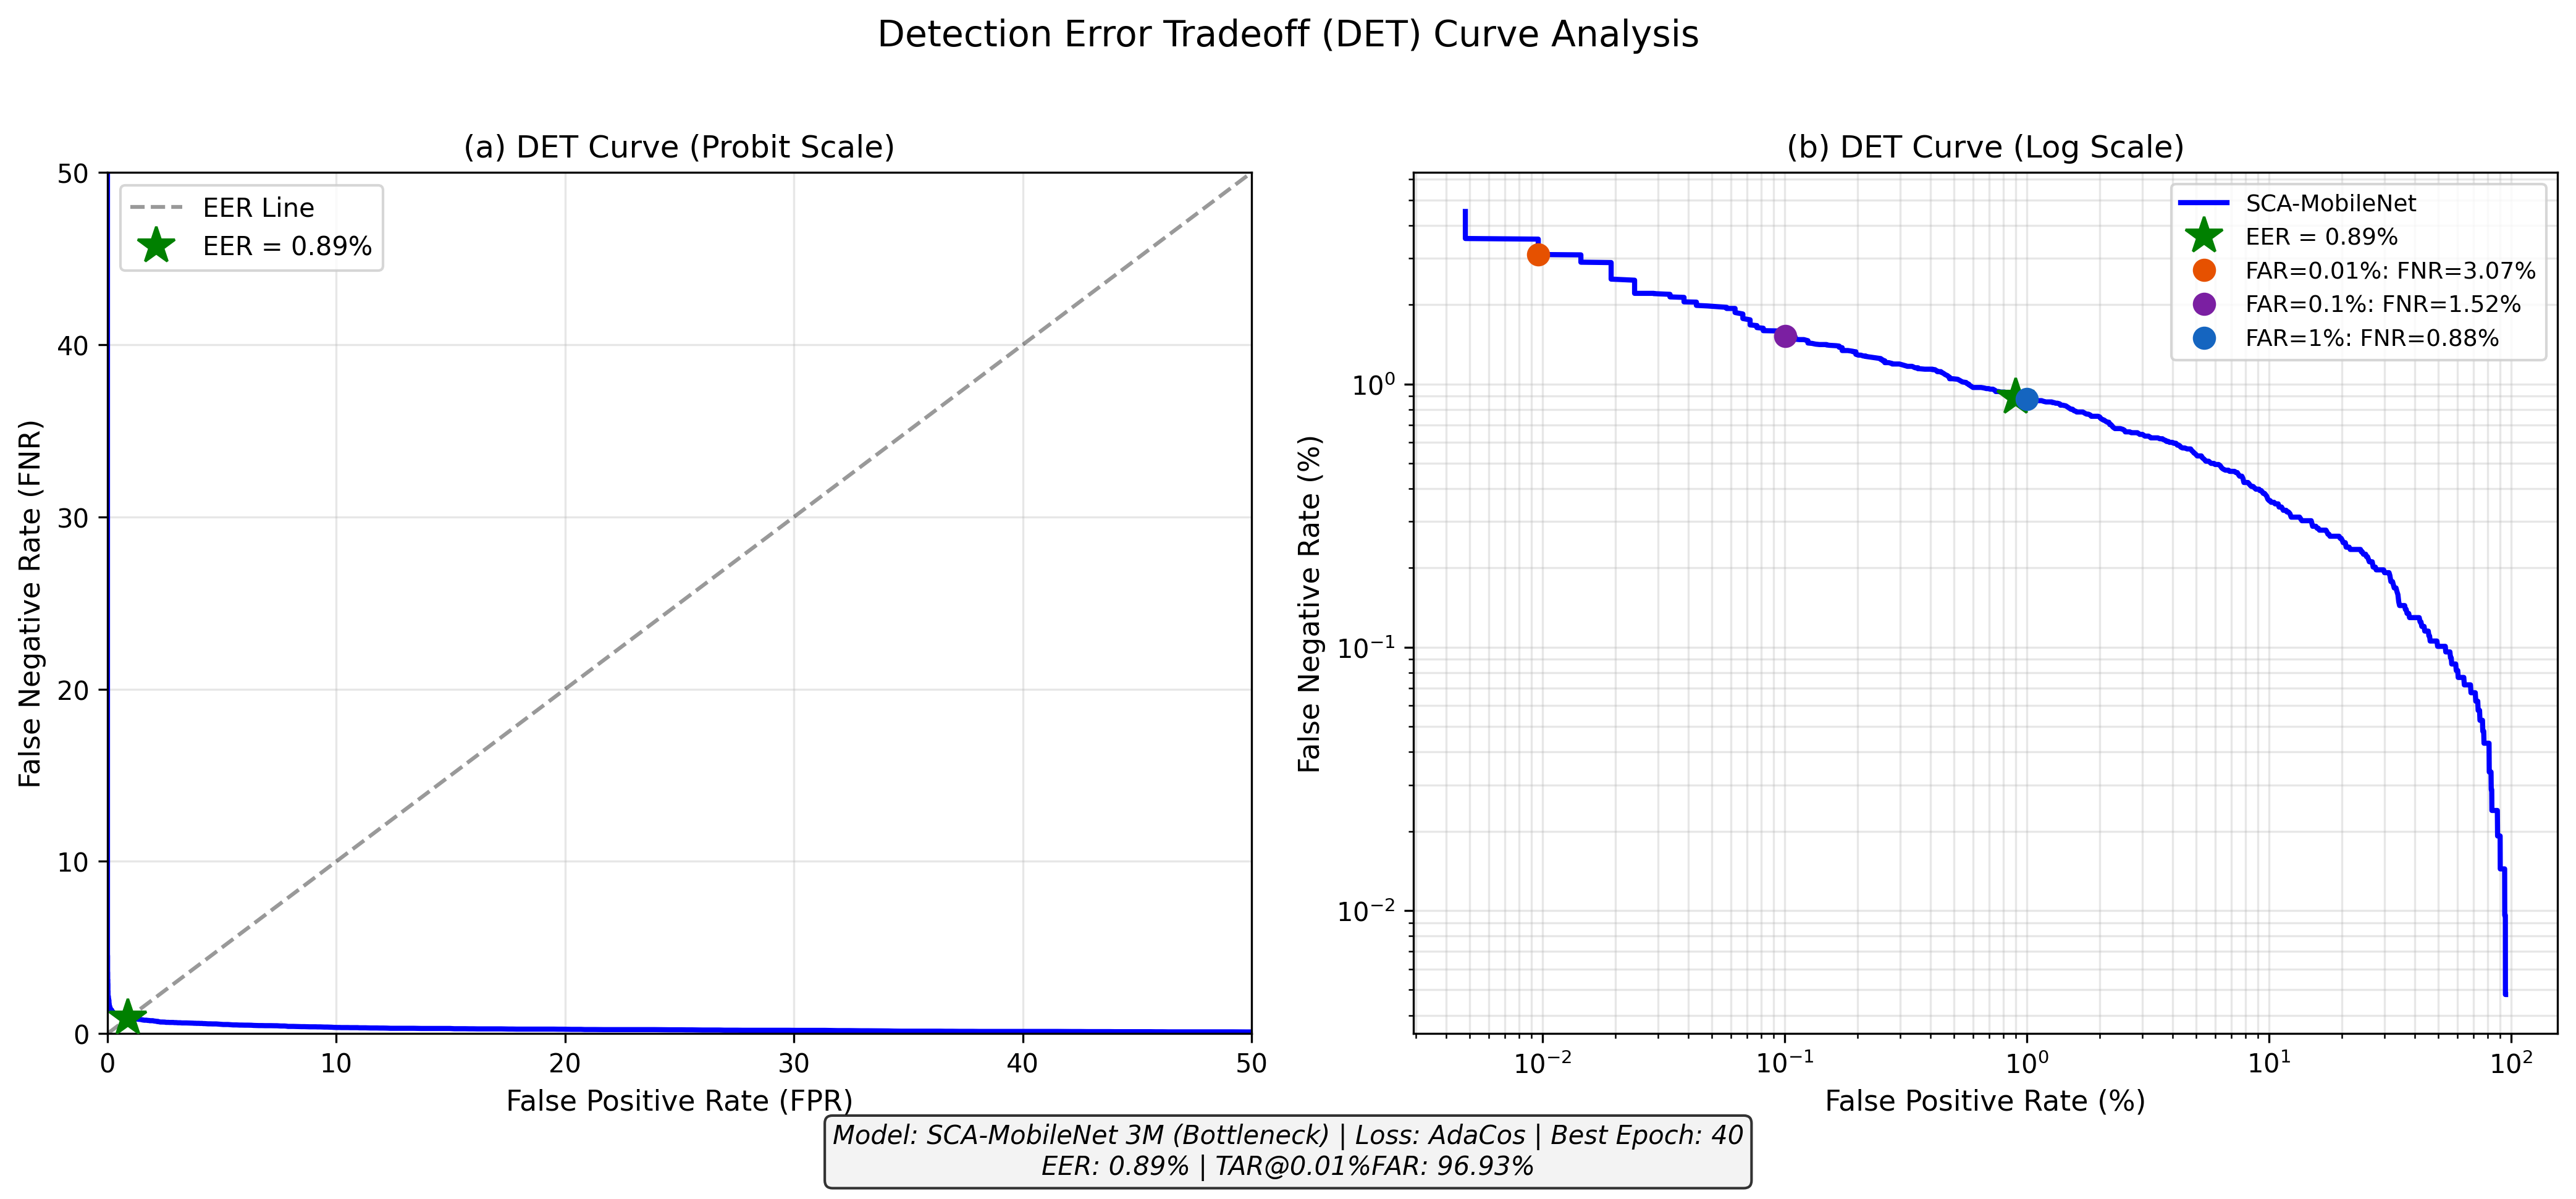
\includegraphics[width=\columnwidth]{fig_det.png}}
\caption{Đường cong DET (Detection Error Tradeoff) trên thang đo logarit theo chuẩn ISO/IEC 19795. Giao điểm FMR = FNMR xác định EER = 0,89\%.}
\label{fig:det}
\end{figure}

\begin{figure}[H]
\centerline{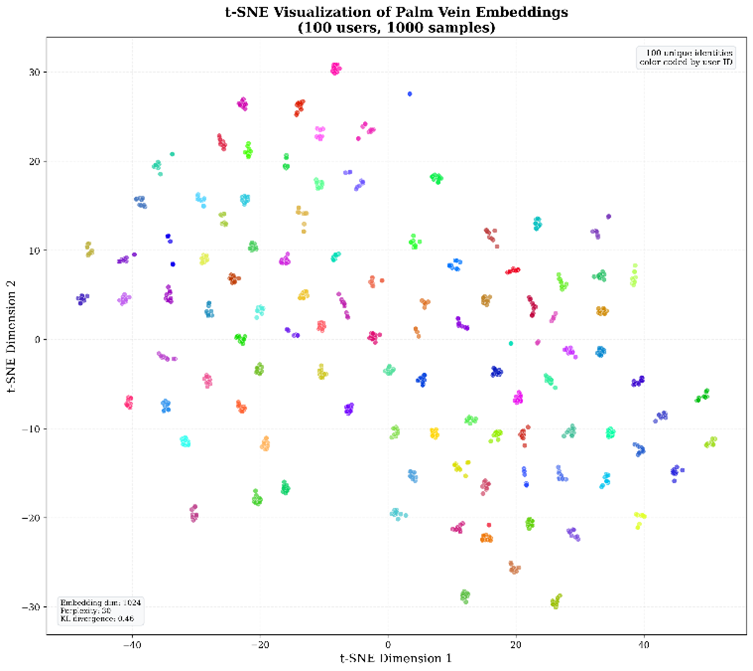
\includegraphics[width=\columnwidth]{fig_tsne.png}}
\caption{Trực quan hóa t-SNE của không gian embedding 1024 chiều trên tập kiểm thử. Mỗi màu đại diện một định danh. SCA-MobileNet tạo ra các cụm (cluster) tách biệt rõ ràng, phản ánh chất lượng phân biệt cao của không gian metric.}
\label{fig:tsne}
\end{figure}

\begin{figure}[H]
\centerline{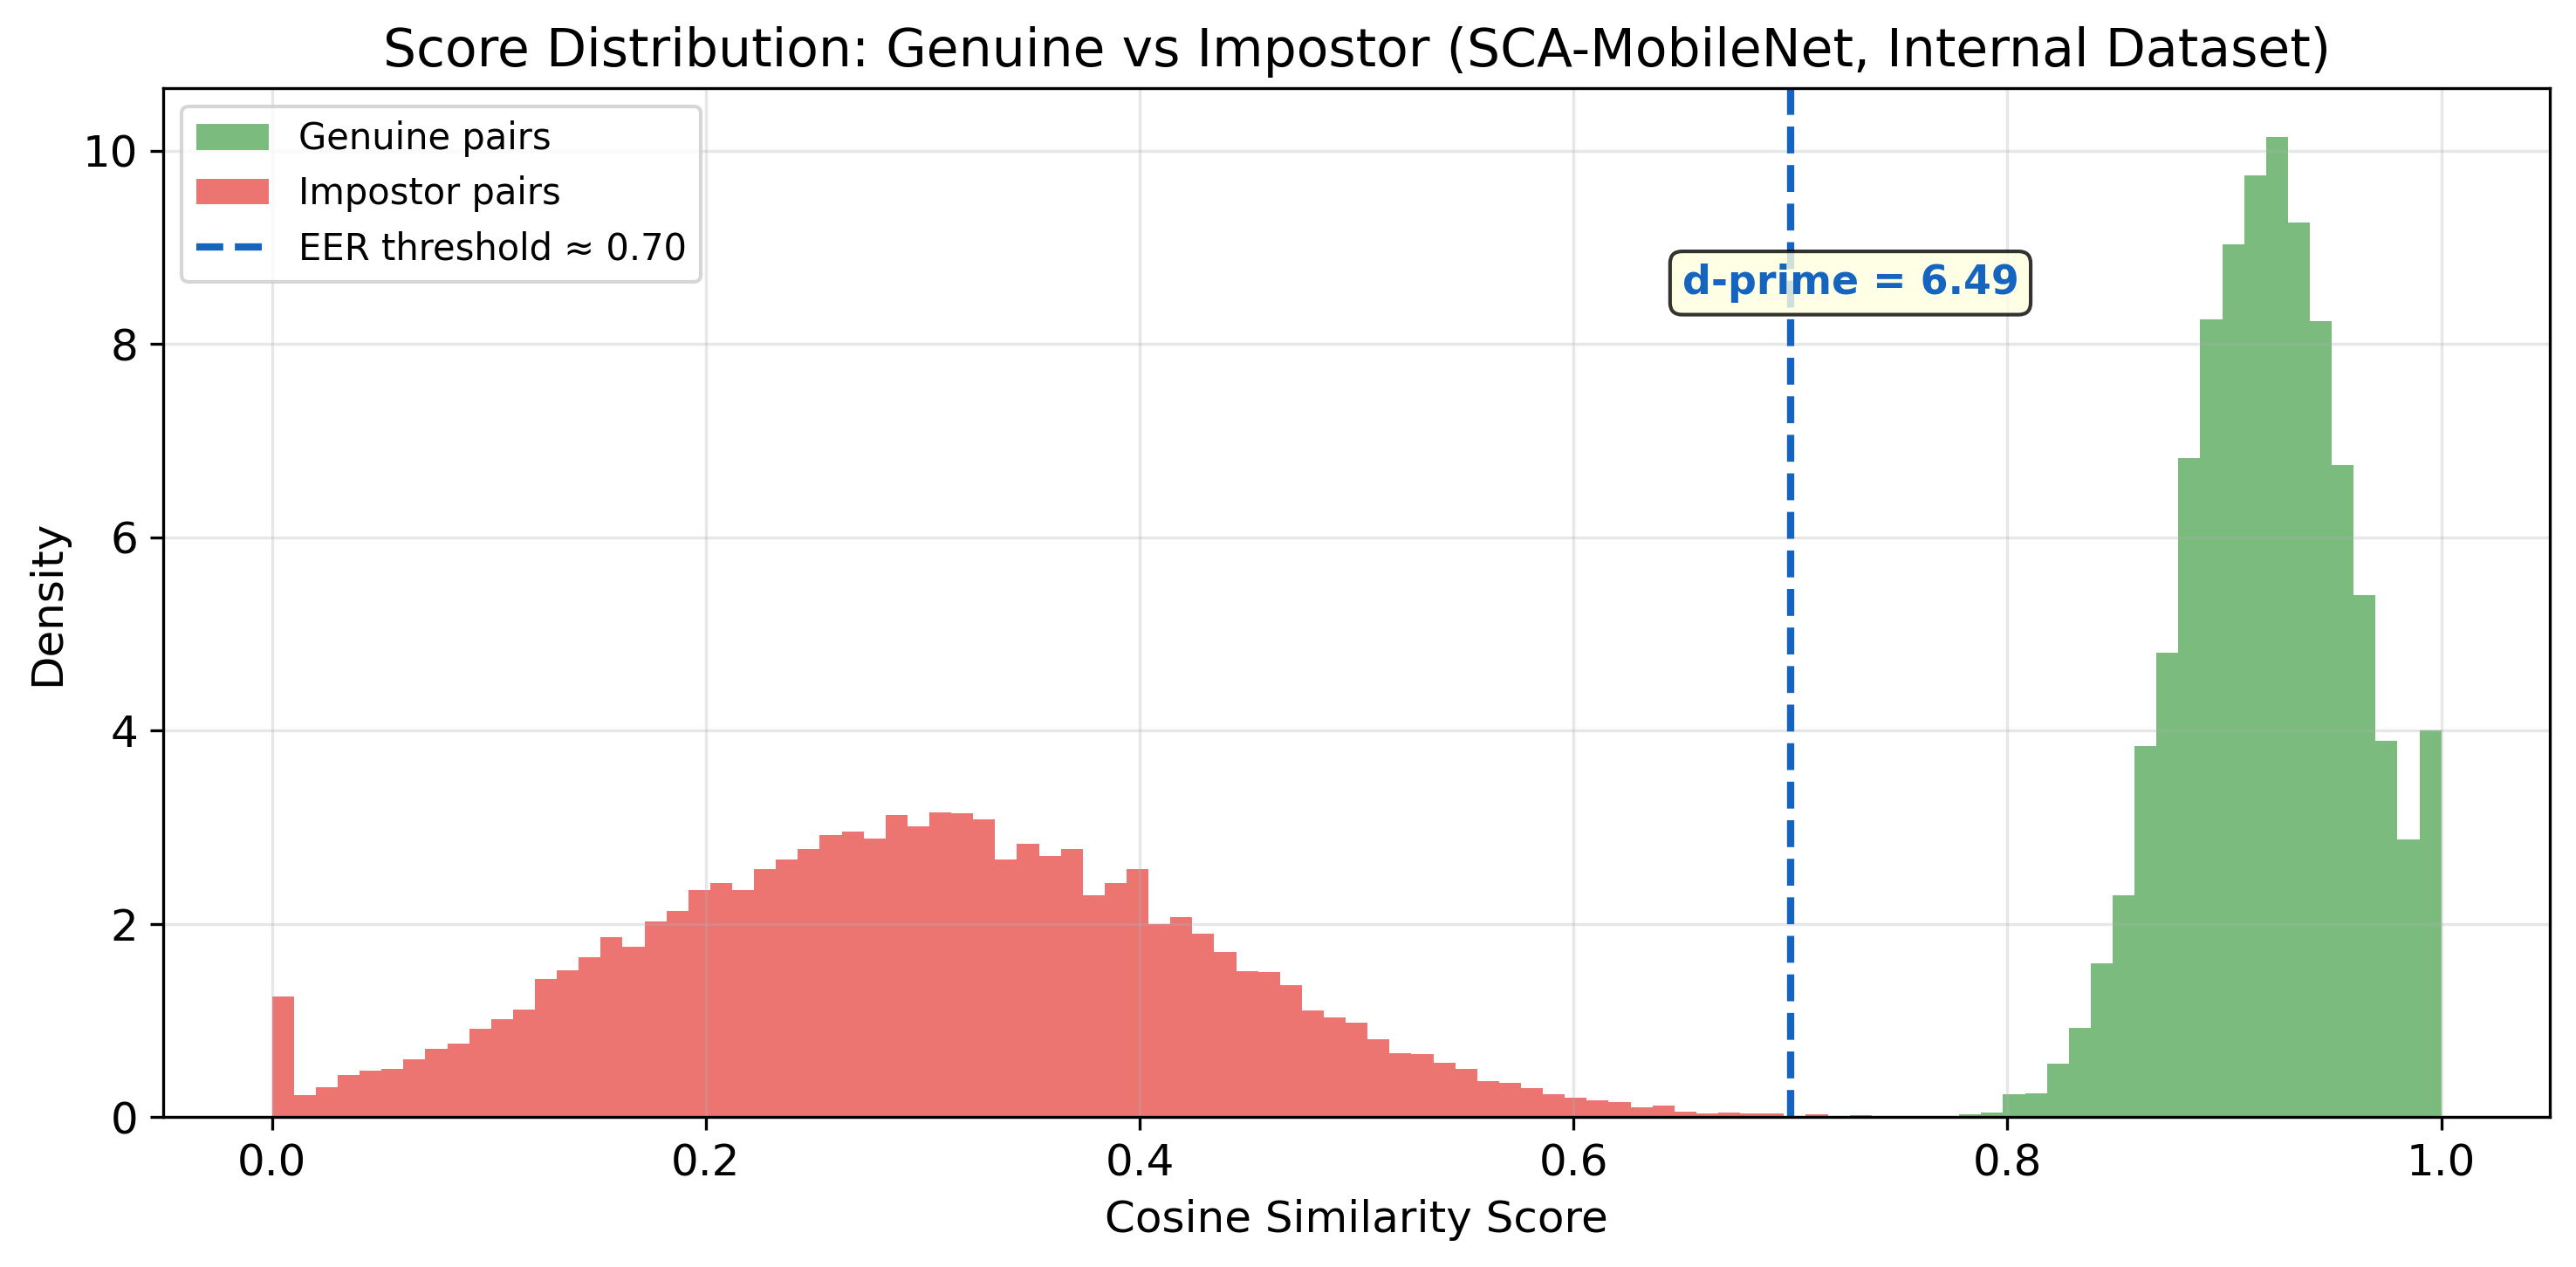
\includegraphics[width=\textwidth]{fig_score_distribution.png}}
\caption{Phân bố điểm tương đồng cosine giữa các cặp genuine và impostor. Hai phân bố tách biệt với vùng chồng lấp nhỏ, phản ánh d-prime cao và EER thấp. Đường đứt nét: ngưỡng EER.}
\label{fig:score_distribution}
\end{figure}

Đường cong ROC cho thấy TAR duy trì ở mức cao trên dải rộng FAR. Tại FAR $\leq 0.01\%$, SCA-MobileNet vẫn đạt TAR cao, phản ánh sự tách biệt rõ ràng giữa phân bố genuine và impostor.

Đường cong DET xác nhận EER 0,89\%. Trên thang logarit, đường cong đơn điệu và ổn định, cho thấy mô hình duy trì hiệu năng tốt tại các điểm vận hành có yêu cầu bảo mật cao (TAR 96,93\% tại FAR = 0,01\%).

\subsection{Tổng hợp Kết quả Toàn diện}

Bảng~\ref{tab:comprehensive_summary} tổng hợp hiệu năng của SCA-MobileNet trên tất cả các kịch bản thực nghiệm, bao gồm huấn luyện trực tiếp trên bốn bộ dữ liệu và ba thí nghiệm cross-domain. Kết quả cho thấy SCA-MobileNet đạt EER thấp nhất nhất quán trên mọi kịch bản.

\begin{table}[H]
\caption{Tổng hợp hiệu năng SCA-MobileNet trên tất cả các kịch bản thực nghiệm. ``Train$\rightarrow$Test'' chỉ kịch bản cross-domain (không fine-tuning).}
\begin{center}
\resizebox{\textwidth}{!}{%
\begin{tabular}{l|c|c|c|c|c|c|l}
\hline
\textbf{Kịch bản} & \textbf{EER (\%)} & \textbf{TAR@0.01\%} & \textbf{TAR@0.1\%} & \textbf{TAR@1\%} & \textbf{AUC} & \textbf{d-prime} & \textbf{Xếp hạng} \\
\hline
\multicolumn{8}{|c|}{\textbf{Huấn luyện trực tiếp (In-domain)}} \\
\hline
Nội bộ (1.549 IDs) & \textbf{0.89} & 96.93\% & 98.49\% & 99.12\% & 0.9983 & 6.49 & \#1 / 12 models \\
TONGJI (1.200 IDs) & \textbf{0.06} & 90.06\% & 99.95\% & 100.0\% & 0.9999 & 8.56 & \#1 / 12 models \\
SCUT (1.100 IDs) & \textbf{1.48} & 88.10\% & 95.00\% & 98.10\% & 0.9986 & 4.83 & \#1 / 12 models \\
VERA (220 IDs) & \textbf{2.76} & 86.20\% & 90.90\% & 95.60\% & 0.9950 & 4.08 & \#1 / 12 models \\
\hline
\multicolumn{8}{|c|}{\textbf{Đánh giá liên miền (Cross-domain, không fine-tuning)}} \\
\hline
Nội bộ $\rightarrow$ TONGJI & \textbf{1.50} & 71.84\% & 94.46\% & --- & 0.9981 & --- & \#1 / 6 models \\
VERA $\rightarrow$ SCUT & \textbf{10.13} & 47.53\% & 56.94\% & 73.10\% & 0.9615 & 2.61 & \#1 / 12 models \\
SCUT $\rightarrow$ VERA & \textbf{5.61} & 78.07\% & 82.28\% & 88.50\% & 0.9814 & 3.38 & \#1 / 12 models \\
\hline
\end{tabular}%
}
\label{tab:comprehensive_summary}
\end{center}
\end{table}

Từ bảng tổng hợp, các nhận xét chính:
\begin{enumerate}
    \item \textbf{In-domain}: SCA-MobileNet đạt EER dưới 3\% trên cả bốn bộ dữ liệu, thấp nhất 0,06\% trên TONGJI. Hiệu năng tương quan với quy mô dữ liệu: TONGJI (840 train IDs, EER 0,06\%) $>$ Nội bộ (1.084 IDs, EER 0,89\%) $>$ SCUT (770 IDs, EER 1,48\%) $>$ VERA (154 IDs, EER 2,76\%).
    \item \textbf{Cross-domain}: EER tăng khi chuyển miền (1,50\% $\rightarrow$ 5,61--10,13\%) do khác biệt phân phối dữ liệu. SCA-MobileNet dẫn đầu với khoảng cách đáng kể trong mọi kịch bản.
    \item \textbf{Tính nhất quán}: SCA-MobileNet xếp hạng \#1 trong tất cả 7 kịch bản (4 in-domain + 3 cross-domain).
\end{enumerate}

\subsection{Phân tích Hiệu quả Tính toán}

Bảng~\ref{tab:inference_benchmark} so sánh chi phí tính toán của tất cả các mô hình, bao gồm số tham số, FLOPs, và thời gian suy luận trên GPU (NVIDIA RTX 4050 Laptop) và CPU (Intel Core). Đo trung bình trên 500 ảnh đầu vào, warmup 100 ảnh.

\begin{table}[H]
\caption{So sánh độ phức tạp tính toán và thời gian suy luận của tất cả các mô hình. Đo trên RTX 4050 Laptop GPU, batch size = 1.}
\begin{center}
\resizebox{\textwidth}{!}{%
\begin{tabular}{l|c|c|c|c|c}
\hline
\textbf{Model} & \textbf{Params (M)} & \textbf{FLOPs (G)} & \textbf{GPU (ms)} & \textbf{CPU (ms)} & \textbf{FPS (GPU)} \\
\hline
MobileNetV3 (Base) & 1,52 & 0,06 & 6,84 & 31,29 & 146,3 \\
MPSNet & 2,99 & 0,14 & 4,88 & 32,92 & 204,9 \\
\textbf{SCA-MobileNet (Ours)} & \textbf{3,19} & \textbf{0,13} & \textbf{10,01} & \textbf{36,87} & \textbf{99,9} \\
EfficientNet-B0 & 4,01 & 0,38 & 11,43 & 66,22 & 87,5 \\
MobileViT-S & 4,94 & 1,83 & 11,87 & 106,67 & 84,3 \\
DeiT-Tiny & 5,52 & 1,07 & 6,88 & 49,55 & 145,3 \\
FGFNet & 5,62 & 6,37 & 23,82 & 325,51 & 42,0 \\
RSNet & 6,23 & 1,17 & 10,22 & 87,56 & 97,8 \\
GSCL (ResNet-18) & 11,23 & 1,82 & --- & --- & --- \\
ResNet-50 & 23,51 & 4,13 & 7,92 & 119,29 & 126,2 \\
Swin-Tiny & 27,52 & 4,37 & 14,27 & 183,50 & 70,1 \\
Modified-DenseNet161 & 28,74 & 7,95 & 29,91 & 312,64 & 33,4 \\
\hline
\end{tabular}%
}
\label{tab:inference_benchmark}
\end{center}
\end{table}

SCA-MobileNet đạt 0,13G FLOPs --- thấp nhất trong nhóm mô hình có EER dưới 2\% --- và thời gian suy luận 10,01~ms/ảnh trên GPU (99,9 FPS), 36,87~ms trên CPU. So với Modified-DenseNet161 (EER tương đương 1,51\%), SCA-MobileNet nhanh hơn 3$\times$ trên GPU và 8,5$\times$ trên CPU, với chỉ 11\% số tham số. MPSNet có latency thấp nhất (4,88~ms GPU) nhưng EER cao hơn (1,57\% trên SCUT).

\subsection{Thảo luận}

\begin{figure}[H]
\centerline{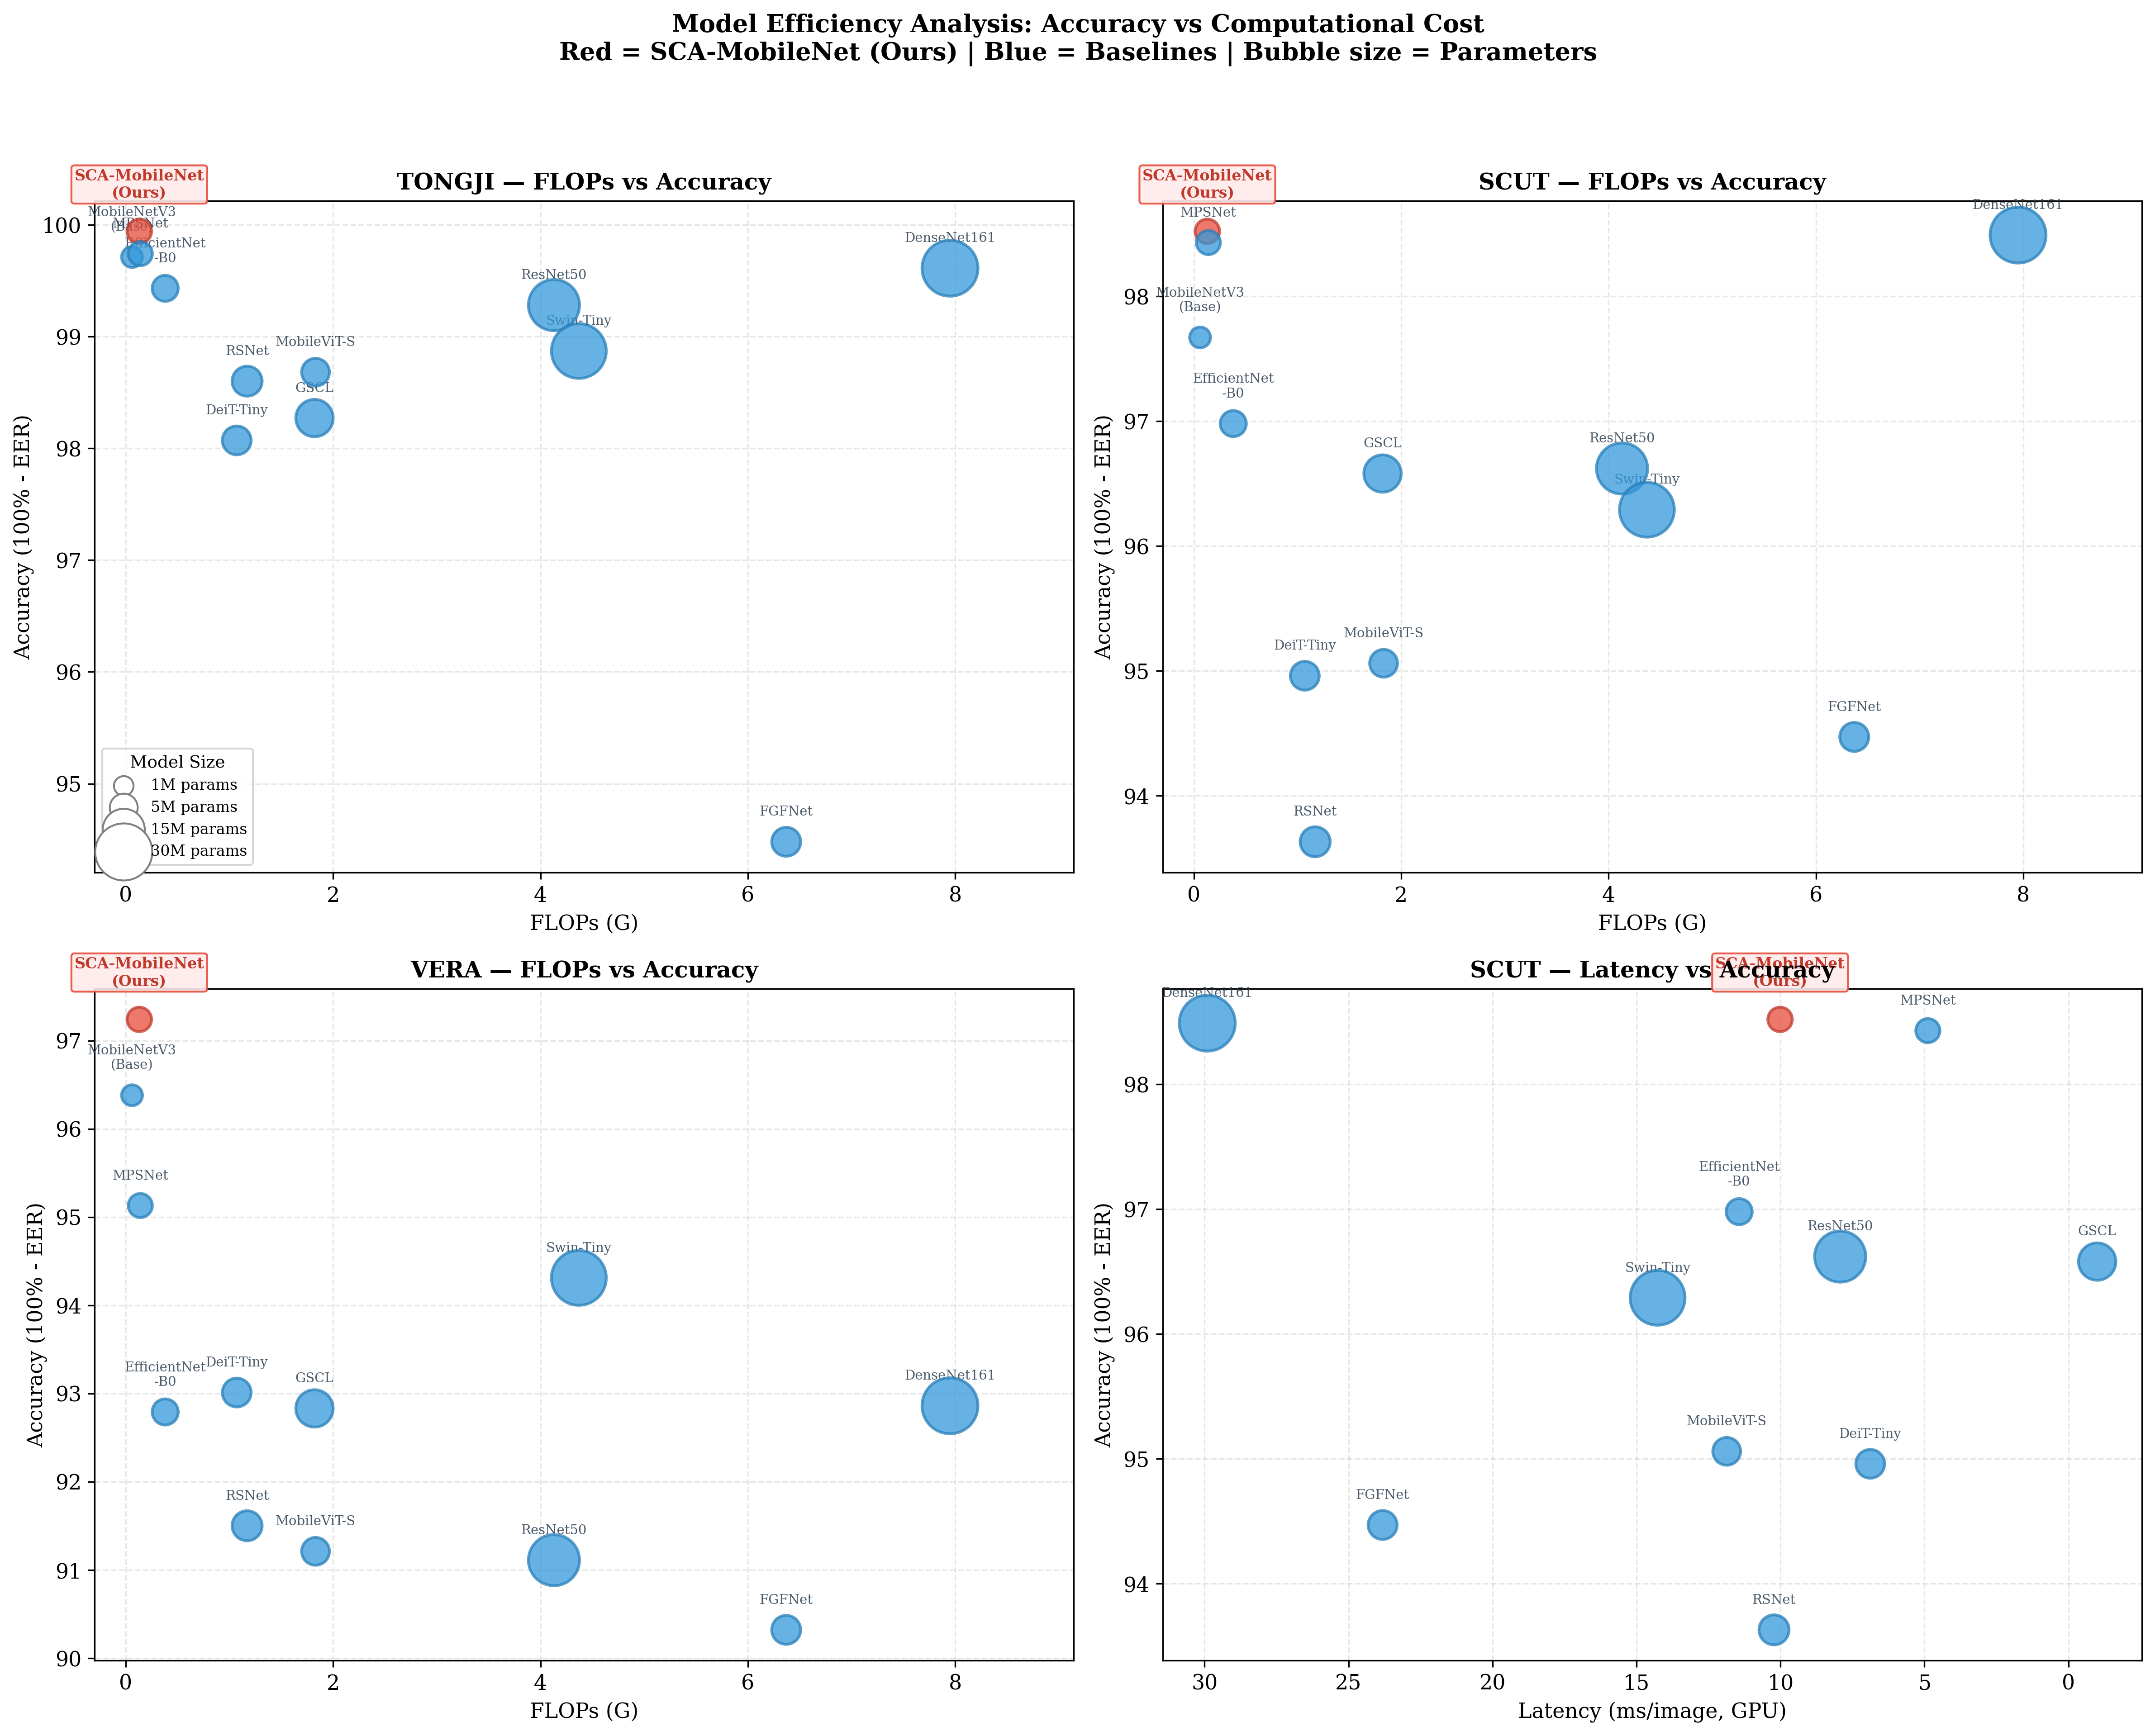
\includegraphics[width=\textwidth]{fig_efficiency_bubble.png}}
\caption{Phân tích hiệu quả mô hình: Accuracy (100\% $-$ EER) so với FLOPs (G) trên ba bộ dữ liệu TONGJI, SCUT, VERA, và Latency (ms) trên SCUT. Kích thước bong bóng tỷ lệ với số tham số. SCA-MobileNet (đỏ) đạt accuracy cao nhất với FLOPs và latency thấp.}
\label{fig:efficiency_bubble}
\end{figure}

Phần này phân tích tổng hợp các kết quả thực nghiệm.

\textbf{Tại sao SCIB hoạt động tốt?} Ablation study (Bảng~\ref{tab:ablation}) cho thấy kết hợp STN+CA+SPP không đơn thuần cộng tuyến tính. Cấu hình STN+CA (Cấu hình 5) cho EER 1,05\% --- cao hơn cả khi dùng riêng lẻ. SPP đóng vai trò cung cấp không gian phân giải đa thang đo cho STN và CA hoạt động hiệu quả; thiếu SPP, hai cơ chế căn chỉnh tọa độ xung đột trên cùng không gian pooling tuyến tính.

\textbf{Hiệu quả tham số và tính toán:} Hình~\ref{fig:efficiency_bubble} và Bảng~\ref{tab:inference_benchmark} cho thấy SCA-MobileNet (3,19M params, 0,13G FLOPs) đạt EER thấp nhất trên mọi bộ dữ liệu, vượt các mô hình có nhiều tham số hơn (Swin-Tiny 27,52M, GSCL 11,23M, RSNet 6,23M). Với thời gian suy luận 10,01~ms trên GPU (99,9 FPS) và 36,87~ms trên CPU, SCA-MobileNet đáp ứng yêu cầu thời gian thực cho triển khai trên thiết bị biên. Kết quả cho thấy kiến trúc nhỏ gọn với inductive bias phù hợp có thể đạt hiệu năng cao hơn backbone tổng quát kích thước lớn.

\textbf{Tổng quát hóa liên miền:} SCA-MobileNet dẫn đầu trên cả ba kịch bản cross-domain (NIR$\rightarrow$TONGJI: EER 1,50\%, SCUT$\rightarrow$VERA: EER 5,61\%, VERA$\rightarrow$SCUT: EER 10,13\%). Khoảng cách lớn với baseline cho thấy SCIB học biểu diễn hình học tổng quát thay vì đặc trưng quang phổ cụ thể.

\textbf{Ảnh hưởng quy mô dữ liệu:} EER tương quan với số định danh huấn luyện. Tuy nhiên, bộ nội bộ (1.084 IDs) có EER cao hơn TONGJI (840 IDs), phản ánh độ khó nội tại do biến thiên tư thế và khoảng cách thu nhận không tiếp xúc.

\textbf{Giới hạn:} (1) Bộ dữ liệu nội bộ chưa công bố công khai do hạn chế quyền riêng tư. (2) Chưa có thí nghiệm phát hiện tấn công giả mạo (\textit{presentation attack detection}). (3) Thí nghiệm cross-domain chưa bao gồm fine-tuning trên miền đích.

%% ====== SECTION VI ======
\section{Kết luận}

Nghiên cứu này đề xuất SCA-MobileNet, một kiến trúc xác thực tĩnh mạch lòng bàn tay không tiếp xúc theo giao thức open-set, giải quyết vấn đề biến thiên tỷ lệ hình học do khoảng cách thu nhận thay đổi.

Hệ thống bao gồm hai thành phần: (1) quy trình tiền xử lý sử dụng phép biến đổi khoảng cách để chuẩn hóa tỷ lệ ROI; và (2) kiến trúc mạng với khối SCIB (Scale-Coordinate Invariant Block) trên nền MobileNetV3-Small. SCIB tích hợp tuần tự STN (chuẩn hóa hình học), Coordinate Attention (định vị cấu trúc theo tọa độ), và SPP (biểu diễn đa thang đo), kết hợp hàm mất mát AdaCos tự thích nghi.

Kết quả thực nghiệm trên bốn bộ dữ liệu: EER 0,89\% trên bộ nội bộ (1.549 ID, TAR 96,93\% tại FAR = 0,01\%), EER 0,06\% trên TONGJI, EER 1,48\% $\pm$ 0,04\% trên SCUT (5 seeds), và EER 2,76\% trên VERA --- xếp hạng \#1 trên tất cả 7 kịch bản (4 in-domain + 3 cross-domain). Toàn bộ kiến trúc gồm 3,19M tham số và 0,13G FLOPs, với thời gian suy luận 10,01~ms/ảnh trên GPU (99,9 FPS) và 36,87~ms trên CPU.

\textbf{Hướng phát triển:} (1) Tích hợp module phát hiện tấn công giả mạo (\textit{presentation attack detection}) dựa trên phân tích tần số. (2) Mở rộng sang cơ chế học liên kết bảo toàn quyền riêng tư (\textit{federated learning}) để triển khai quy mô lớn mà không chia sẻ dữ liệu sinh trắc.

\begin{thebibliography}{00}
\bibitem{b_covid1} R. W. T. Lee et al., ``Contactless biometrics in the post-COVID era: A systematic review,'' \textit{IEEE Access}, vol. 9, pp. 129202--129231, 2021.
\bibitem{b_covid2} T. Nguyen, ``Palm vein recognition for hygienic access control,'' \textit{Security Journal}, vol. 35, no. 2, pp. 240--255, 2022.
\bibitem{b18} D. Zhang et al., ``Online palmprint identification,'' \textit{IEEE Transactions on Pattern Analysis and Machine Intelligence}, 2003.
\bibitem{b19} A. K. Jain, A. Ross, and S. Prabhakar, ``An introduction to biometric recognition,'' \textit{IEEE Transactions on Circuits and Systems for Video Technology}, 2004.
\bibitem{b12} W. J. Scheirer, A. de Rezende Rocha, A. Sapkota, and T. E. Boult, ``Toward open set recognition,'' \textit{IEEE Transactions on Pattern Analysis and Machine Intelligence}, vol. 35, no. 7, pp. 1757-1772, 2013.
\bibitem{b13} A. Bendale and T. E. Boult, ``Towards open set deep networks,'' in \textit{Proceedings of the IEEE Conference on Computer Vision and Pattern Recognition (CVPR)}, 2016, pp. 1563-1572.
\bibitem{b_closedset} Y. Wen, K. Zhang, Z. Li, and Y. Qiao, ``A discriminative feature learning approach for deep face recognition,'' in \textit{European Conference on Computer Vision (ECCV)}, 2016.
\bibitem{b1} W. Horng et al., ``A robust contactless palm vein recognition system using RGB images,'' \textit{IEEE Access}, 2022.
\bibitem{b4} P. Li et al., ``RSNet: Region-specific modeling for contactless palm vein recognition,'' \textit{IEEE Transactions on Information Forensics and Security}, 2024.
\bibitem{b9} M. Jaderberg, K. Simonyan, A. Zisserman, and K. Kavukcuoglu, ``Spatial transformer networks,'' in \textit{Advances in Neural Information Processing Systems}, vol. 28, 2015.
\bibitem{b7} Q. Hou, D. Zhou, and J. Feng, ``Coordinate attention for efficient mobile network design,'' in \textit{Proceedings of the IEEE/CVF Conference on Computer Vision and Pattern Recognition (CVPR)}, 2021.
\bibitem{b8} K. He, X. Zhang, S. Ren, and J. Sun, ``Spatial pyramid pooling in deep convolutional networks for visual recognition,'' \textit{IEEE Transactions on Pattern Analysis and Machine Intelligence}, vol. 37, no. 9, pp. 1904-1916, 2015.
\bibitem{b11} H. Wang et al., ``AdaCos: Adaptively scaling cosine logits for effectively learning deep face representations,'' in \textit{Proceedings of the IEEE/CVF Conference on Computer Vision and Pattern Recognition (CVPR)}, 2019.
\bibitem{b2} R. S. Kuzu, E. Piciucco, E. Maiorana, and P. Campisi, ``On-the-fly finger-vein-based biometric recognition using deep neural networks,'' \textit{IEEE Transactions on Information Forensics and Security}, 2020.
\bibitem{b14} J. Deng, J. Guo, N. Xue, and S. Zafeiriou, ``ArcFace: Additive angular margin loss for deep face recognition,'' in \textit{Proceedings of the IEEE/CVF Conference on Computer Vision and Pattern Recognition (CVPR)}, 2019.
\bibitem{b16} W. Liu et al., ``SphereFace: Deep hypersphere embedding for face recognition,'' in \textit{Proceedings of the IEEE Conference on Computer Vision and Pattern Recognition (CVPR)}, 2017.
\bibitem{b15} H. Wang et al., ``CosFace: Large margin cosine loss for deep face recognition,'' in \textit{Proceedings of the IEEE Conference on Computer Vision and Pattern Recognition (CVPR)}, 2018.
\bibitem{b3} Y. Ou et al., ``GSCL: Generative self-supervised contrastive learning for palm vein recognition,'' \textit{Pattern Recognition}, 2023.
\bibitem{b5} G. Kim et al., ``FGFNet: Fourier-guided feature network for presentation attack detection in palm vein recognition,'' \textit{IEEE Transactions on Information Forensics and Security}, 2023.
\bibitem{b21} L. Zhang, L. Li, A. Yang, Y. Shen, and M. Yang, ``Towards contactless palmprint recognition: A novel device, a new benchmark, and a collaborative representation based identification approach,'' \textit{Pattern Recognition}, vol. 69, pp. 199--212, 2017.
\bibitem{b10} A. Howard et al., ``Searching for MobileNetV3,'' in \textit{Proceedings of the IEEE/CVF International Conference on Computer Vision (ICCV)}, 2019, pp. 1314-1324.
\bibitem{b17} ISO/IEC 19795-1:2006, \textit{Information technology---Biometric performance testing and reporting---Part 1: Principles and framework}, International Organization for Standardization, Geneva, Switzerland, 2006.
\bibitem{b20} M. Tan and Q. V. Le, ``EfficientNet: Rethinking model scaling for convolutional neural networks,'' in \textit{Proceedings of the 36th International Conference on Machine Learning (ICML)}, 2019, pp. 6105--6114.
\bibitem{b_scut} L. Zhang, Z. Li, and D. Zhang, ``SCUT FVP: A finger-vein and palmprint database,'' South China University of Technology, 2018. Available: \url{https://github.com/SCUT-BIP-Lab/SCUT-FVP}.
\bibitem{b_vera} P. Tome, R. Raghavendra, C. Busch, et al., ``The 1st competition on counter measures to finger vein spoofing attacks,'' in \textit{IEEE International Conference on Biometrics (ICB)}, 2015. VERA Palmvein Dataset, Idiap Research Institute.
\end{thebibliography}

\end{document}
